% \documentclass[aspectratio=169,onlytextwidth,english]{beamer}
\documentclass[onlytextwidth,english]{beamer}\usepackage[]{graphicx}\usepackage[]{xcolor}
% maxwidth is the original width if it is less than linewidth
% otherwise use linewidth (to make sure the graphics do not exceed the margin)
\makeatletter
\def\maxwidth{ %
  \ifdim\Gin@nat@width>\linewidth
    \linewidth
  \else
    \Gin@nat@width
  \fi
}
\makeatother

\definecolor{fgcolor}{rgb}{0.345, 0.345, 0.345}
\newcommand{\hlnum}[1]{\textcolor[rgb]{0.686,0.059,0.569}{#1}}%
\newcommand{\hlsng}[1]{\textcolor[rgb]{0.192,0.494,0.8}{#1}}%
\newcommand{\hlcom}[1]{\textcolor[rgb]{0.678,0.584,0.686}{\textit{#1}}}%
\newcommand{\hlopt}[1]{\textcolor[rgb]{0,0,0}{#1}}%
\newcommand{\hldef}[1]{\textcolor[rgb]{0.345,0.345,0.345}{#1}}%
\newcommand{\hlkwa}[1]{\textcolor[rgb]{0.161,0.373,0.58}{\textbf{#1}}}%
\newcommand{\hlkwb}[1]{\textcolor[rgb]{0.69,0.353,0.396}{#1}}%
\newcommand{\hlkwc}[1]{\textcolor[rgb]{0.333,0.667,0.333}{#1}}%
\newcommand{\hlkwd}[1]{\textcolor[rgb]{0.737,0.353,0.396}{\textbf{#1}}}%
\let\hlipl\hlkwb

\usepackage{framed}
\makeatletter
\newenvironment{kframe}{%
 \def\at@end@of@kframe{}%
 \ifinner\ifhmode%
  \def\at@end@of@kframe{\end{minipage}}%
  \begin{minipage}{\columnwidth}%
 \fi\fi%
 \def\FrameCommand##1{\hskip\@totalleftmargin \hskip-\fboxsep
 \colorbox{shadecolor}{##1}\hskip-\fboxsep
     % There is no \\@totalrightmargin, so:
     \hskip-\linewidth \hskip-\@totalleftmargin \hskip\columnwidth}%
 \MakeFramed {\advance\hsize-\width
   \@totalleftmargin\z@ \linewidth\hsize
   \@setminipage}}%
 {\par\unskip\endMakeFramed%
 \at@end@of@kframe}
\makeatother

\definecolor{shadecolor}{rgb}{.97, .97, .97}
\definecolor{messagecolor}{rgb}{0, 0, 0}
\definecolor{warningcolor}{rgb}{1, 0, 1}
\definecolor{errorcolor}{rgb}{1, 0, 0}
\newenvironment{knitrout}{}{} % an empty environment to be redefined in TeX

\usepackage{alltt}

% use official beamer theme from uzh
\usetheme[english]{uzh} 

% First installation of languages required
% tinytex::tlmgr_install("babel-english")
% tinytex::tlmgr_install("babel-german")


%% load relevant packages:


\usepackage[T1]{fontenc}
\usepackage[latin9]{inputenc}
%\usepackage[english]{babel}
\usepackage{pgfpages}           % necessary for the handouts production
\usepackage{amsmath}            % for nice mathematics
\usepackage{verbatim}           % for verbatim output
\usepackage{wasysym}            % symbols (smilies etc.)
\usepackage{longtable}
\usepackage{float}
\usepackage{textcomp}
\usepackage{graphicx}
\usepackage{xcolor} % for the color names, see: http://en.wikibooks.org/wiki/LaTeX/Colors#Predefined_
\usepackage{natbib}             % for bibliography style and citations
\usepackage{hyperref}
\usepackage{caption}
\hypersetup{%
    hyperindex=true,
    colorlinks=true,%
    urlcolor = {uzh@blue},% in theme uzh
    citecolor = {uzh@blue},
    urlcolor = {uzh@berry},
    pdfstartview=Fit,%
    pdfpagelayout=SinglePage,%
    pdfpagemode=UseThumbs
  }%
\usepackage{url}
\DeclareOptionBeamer{compress}{\beamer@compresstrue}
\ProcessOptionsBeamer

%% define slidetitle color
\setbeamercolor{title}{fg=uzh@blue}
\setbeamercolor{frametitle}{fg=uzh@blue}


% \title{Neural Causal Models with TRAM-DAGs}
\title{\normalsize Functional Modeling with Neural Causal Models and Personalized Treatment Effect Estimation}


%% The following are all optional, simply comment them
%\subtitle{Subtitle (optional)}
\institute{Master Program in Biostatistics www.biostat.uzh.ch\\ Master Thesis: Final Presentation}  %% optional
% leave some vertical space here

\author{Mike Kr{\"a}henb{\"u}hl, Supervisors: Beate Sick, Oliver D{\"u}rr }
\date{\today}
\titlegraphic{img/uzh-lake.jpg}


%%%%%%%%%%%%%%%%%%%%%%%%%%%%%%%%%%%%%%%%%%%%%%%%%%%%%%%% 


\IfFileExists{upquote.sty}{\usepackage{upquote}}{}
\begin{document}

\maketitle




\begin{frame}{Background}

\begin{columns}

% Left side: Text (approx. 3/4 of the slide)
\begin{column}{0.7\textwidth}
\textbf{Supervisors:}
\begin{itemize}
    \item Beate Sick, UZH
    \item Oliver D{\"u}rr, HTWG Konstanz
\end{itemize}

\textbf{Paper \textit{"Interpretable Neural Causal Models with TRAM-DAGs"} \citep{sick2025}:}
\begin{itemize}
    \item Framework to model causal relationships
    \item Based on transformation models
    \item Rely on (deep) neural networks
    \item Compromise between interpretability and flexibility
\end{itemize}
\end{column}

% Right side: Image (approx. 1/4 of the slide)
\begin{column}{0.3\textwidth}
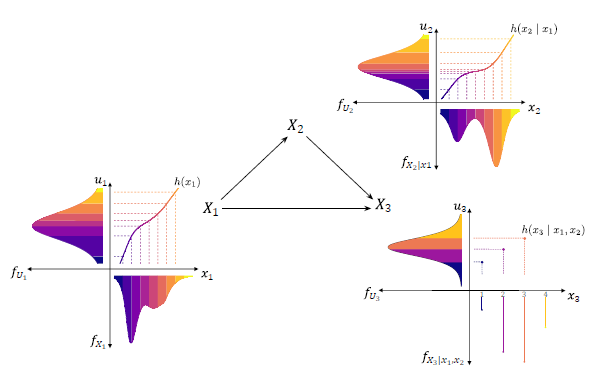
\includegraphics[width=\textwidth]{img/TRAM_DAG_Background.png}
\end{column}

\end{columns}

They showed on synthetic data, that TRAM-DAGs can be fitted on observational data and tackle causal queries on all three levels of Pearl's causal hierarchy.

\end{frame}






\begin{frame}{Research Questions}


\textbf{In this presentation:}


\begin{enumerate}
    \item TRAM-DAGs
    
    \begin{itemize}
        \item How do they work?
    \end{itemize}
    
    \item Individualized Treatment Effect (ITE) estimation
    \begin{itemize}
        \item Does it work on real data (International Stroke Trial)?
        \item When and why does ITE estimation fail (simulation)?
        \item How to estimate ITEs with TRAM-DAGs in a complicated graph (simulation)?
    \end{itemize}
\end{enumerate}
\end{frame}







\begin{frame}{RCT vs. Observational Data}

\vspace{1cm}

\begin{columns}

% Left side: Text
\begin{column}{0.43\textwidth}
\textbf{Randomized Controlled Trial:}
\begin{itemize}
    \item Gold standard for estimating causal effect
    \item Solves problem of confounding
\end{itemize}

\end{column}

% \hspace{0.5cm}

\begin{column}{0.45\textwidth}
\textbf{Observational Data:}
\begin{itemize}
    \item Real world, potential confounding
    \item We assume no unobserved confounding
\end{itemize}
\end{column}

\end{columns}


% Below: image
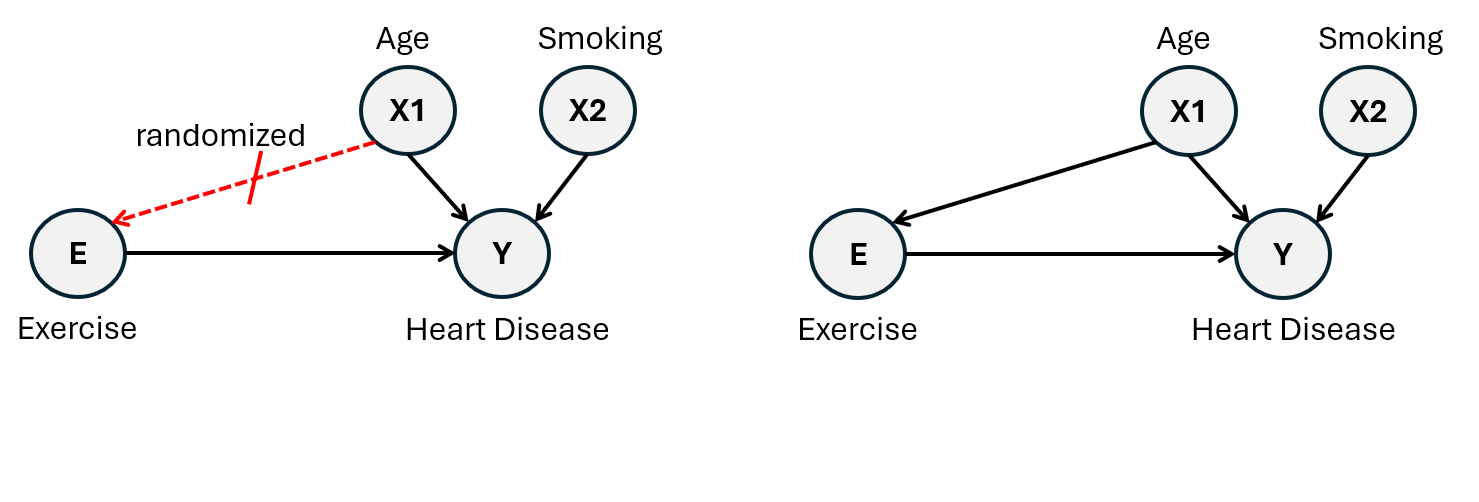
\includegraphics[width=\textwidth]{img/RCT_Observational.png}


\end{frame}




\begin{frame}{Pearl's Causality Ladder}

\begin{columns}

% Left side: Text (60%)
\begin{column}{0.60\textwidth}

\textbf{Observational (seeing)} \\
$P(Y=1 \mid E=1)$ \\
{\footnotesize \textit{"Probability of heart disease given that the person exercises"}}

\vspace{0.4cm}

\textbf{Interventional (doing)} \\
$P(Y=1 \mid \text{do}(E=1))$ \\
{\footnotesize \textit{"Probability of heart disease if we made people start exercising"}} 

\vspace{0.4cm}

\textbf{Counterfactual (imagining)} \\
 $P(Y_{(E=1)} = 1 \mid E=0, Y=1)$ \\
{\footnotesize \textit{"Would someone who does not exercise and has heart disease still have it if they had exercised?"}}

\end{column}

% Right side: Image (40%)
\begin{column}{0.40\textwidth}
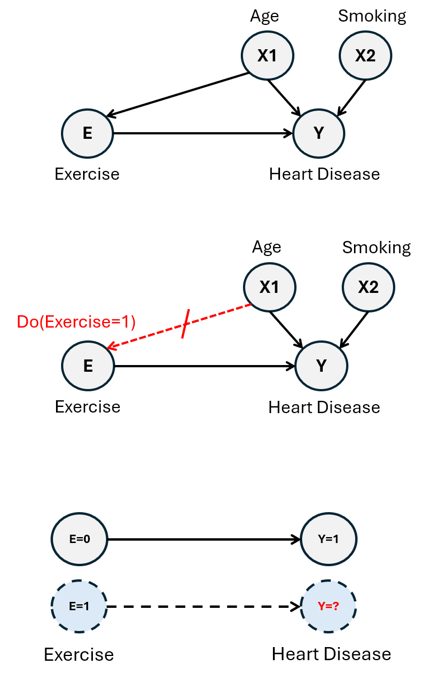
\includegraphics[width=1\linewidth]{img/Pearls_Ladder.png}
\end{column}

\end{columns}

\end{frame}



% 
% \begin{frame}{Causality: Example}
%     \centering
%     \vspace{0.2cm}
% <<dag_smoking, echo=FALSE, fig.width=3, fig.height=3, out.width="40%">>=
% theme_set(theme_dag())
% 
% # Set custom coordinates
% coord_dag <- list(
%   x = c(smoking = 0, age = 1, exercise = 2, heart = 2),
%   y = c(smoking = 1.3, age = 1.5, exercise = 1.5, heart = 1.3)
% )
% 
% smoking_ca_dag <- dagify(heart ~ smoking + age + exercise,
%   smoking ~ age,
%   labels = c(
%     "heart" = "Heart Disease",
%     "smoking" = "Smoking",
%     "exercise" = "Exercise",
%     "age" = "Age"
%   ),
%   #latent = "unhealthy",
%   exposure = "smoking",
%   outcome = "heart",
%   coords = coord_dag
% )
% 
% # plot with reduced size
% ggdag(smoking_ca_dag, text = FALSE, use_labels = "label") + theme_void()
% 
% 
% # Use label repel to avoid overlap with arrows
% ggdag(smoking_ca_dag, text = TRUE) +
% 	geom_dag_label(aes(label = label, fill = FALSE), 
%                   label.size = 0.2,
%                   size = 3.5, 
%                   color = "black", 
%                   segment.color = "black", 
%                   segment.size = 0.2) +
%   theme_void()
% 
% @
% \end{frame}
\begin{frame}{Structural Causal Model}

\textbf{SCM:} Describes the causal mechanism and probabilistic uncertainty

\vspace{0.2cm}

\begin{itemize}
    \item $X_i$ = observed variable
    \item $U_i$ = noise distribution
    % \item $f$ = in our case: $X_2 = f(X_1, U) = h^{-1}(U_{\text{logis}} - \mathbf{x}^\top \boldsymbol{\beta})$
\end{itemize}

\vfill

\centering
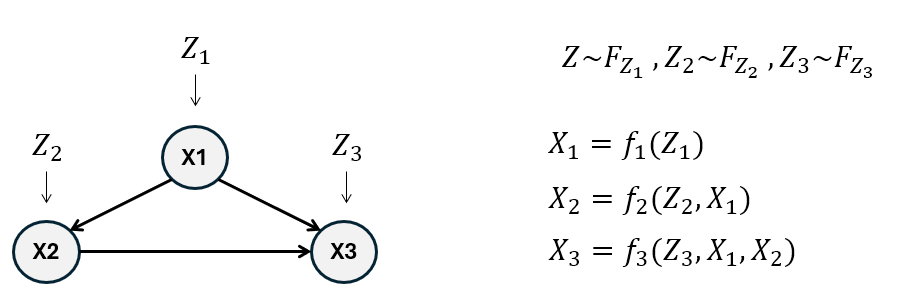
\includegraphics[width=1\textwidth]{img/SCM.png}

\end{frame}






\begin{frame}{Estimating Functional Form}

% Statistical Methods
\begin{columns}
\begin{column}{0.75\textwidth}
\textbf{Statistical methods:}
\begin{itemize}
    \item E.g. linear/logistic regression
    \item Predefined form, risk of bias if misspecified
\end{itemize}
\end{column}
\begin{column}{0.23\textwidth}
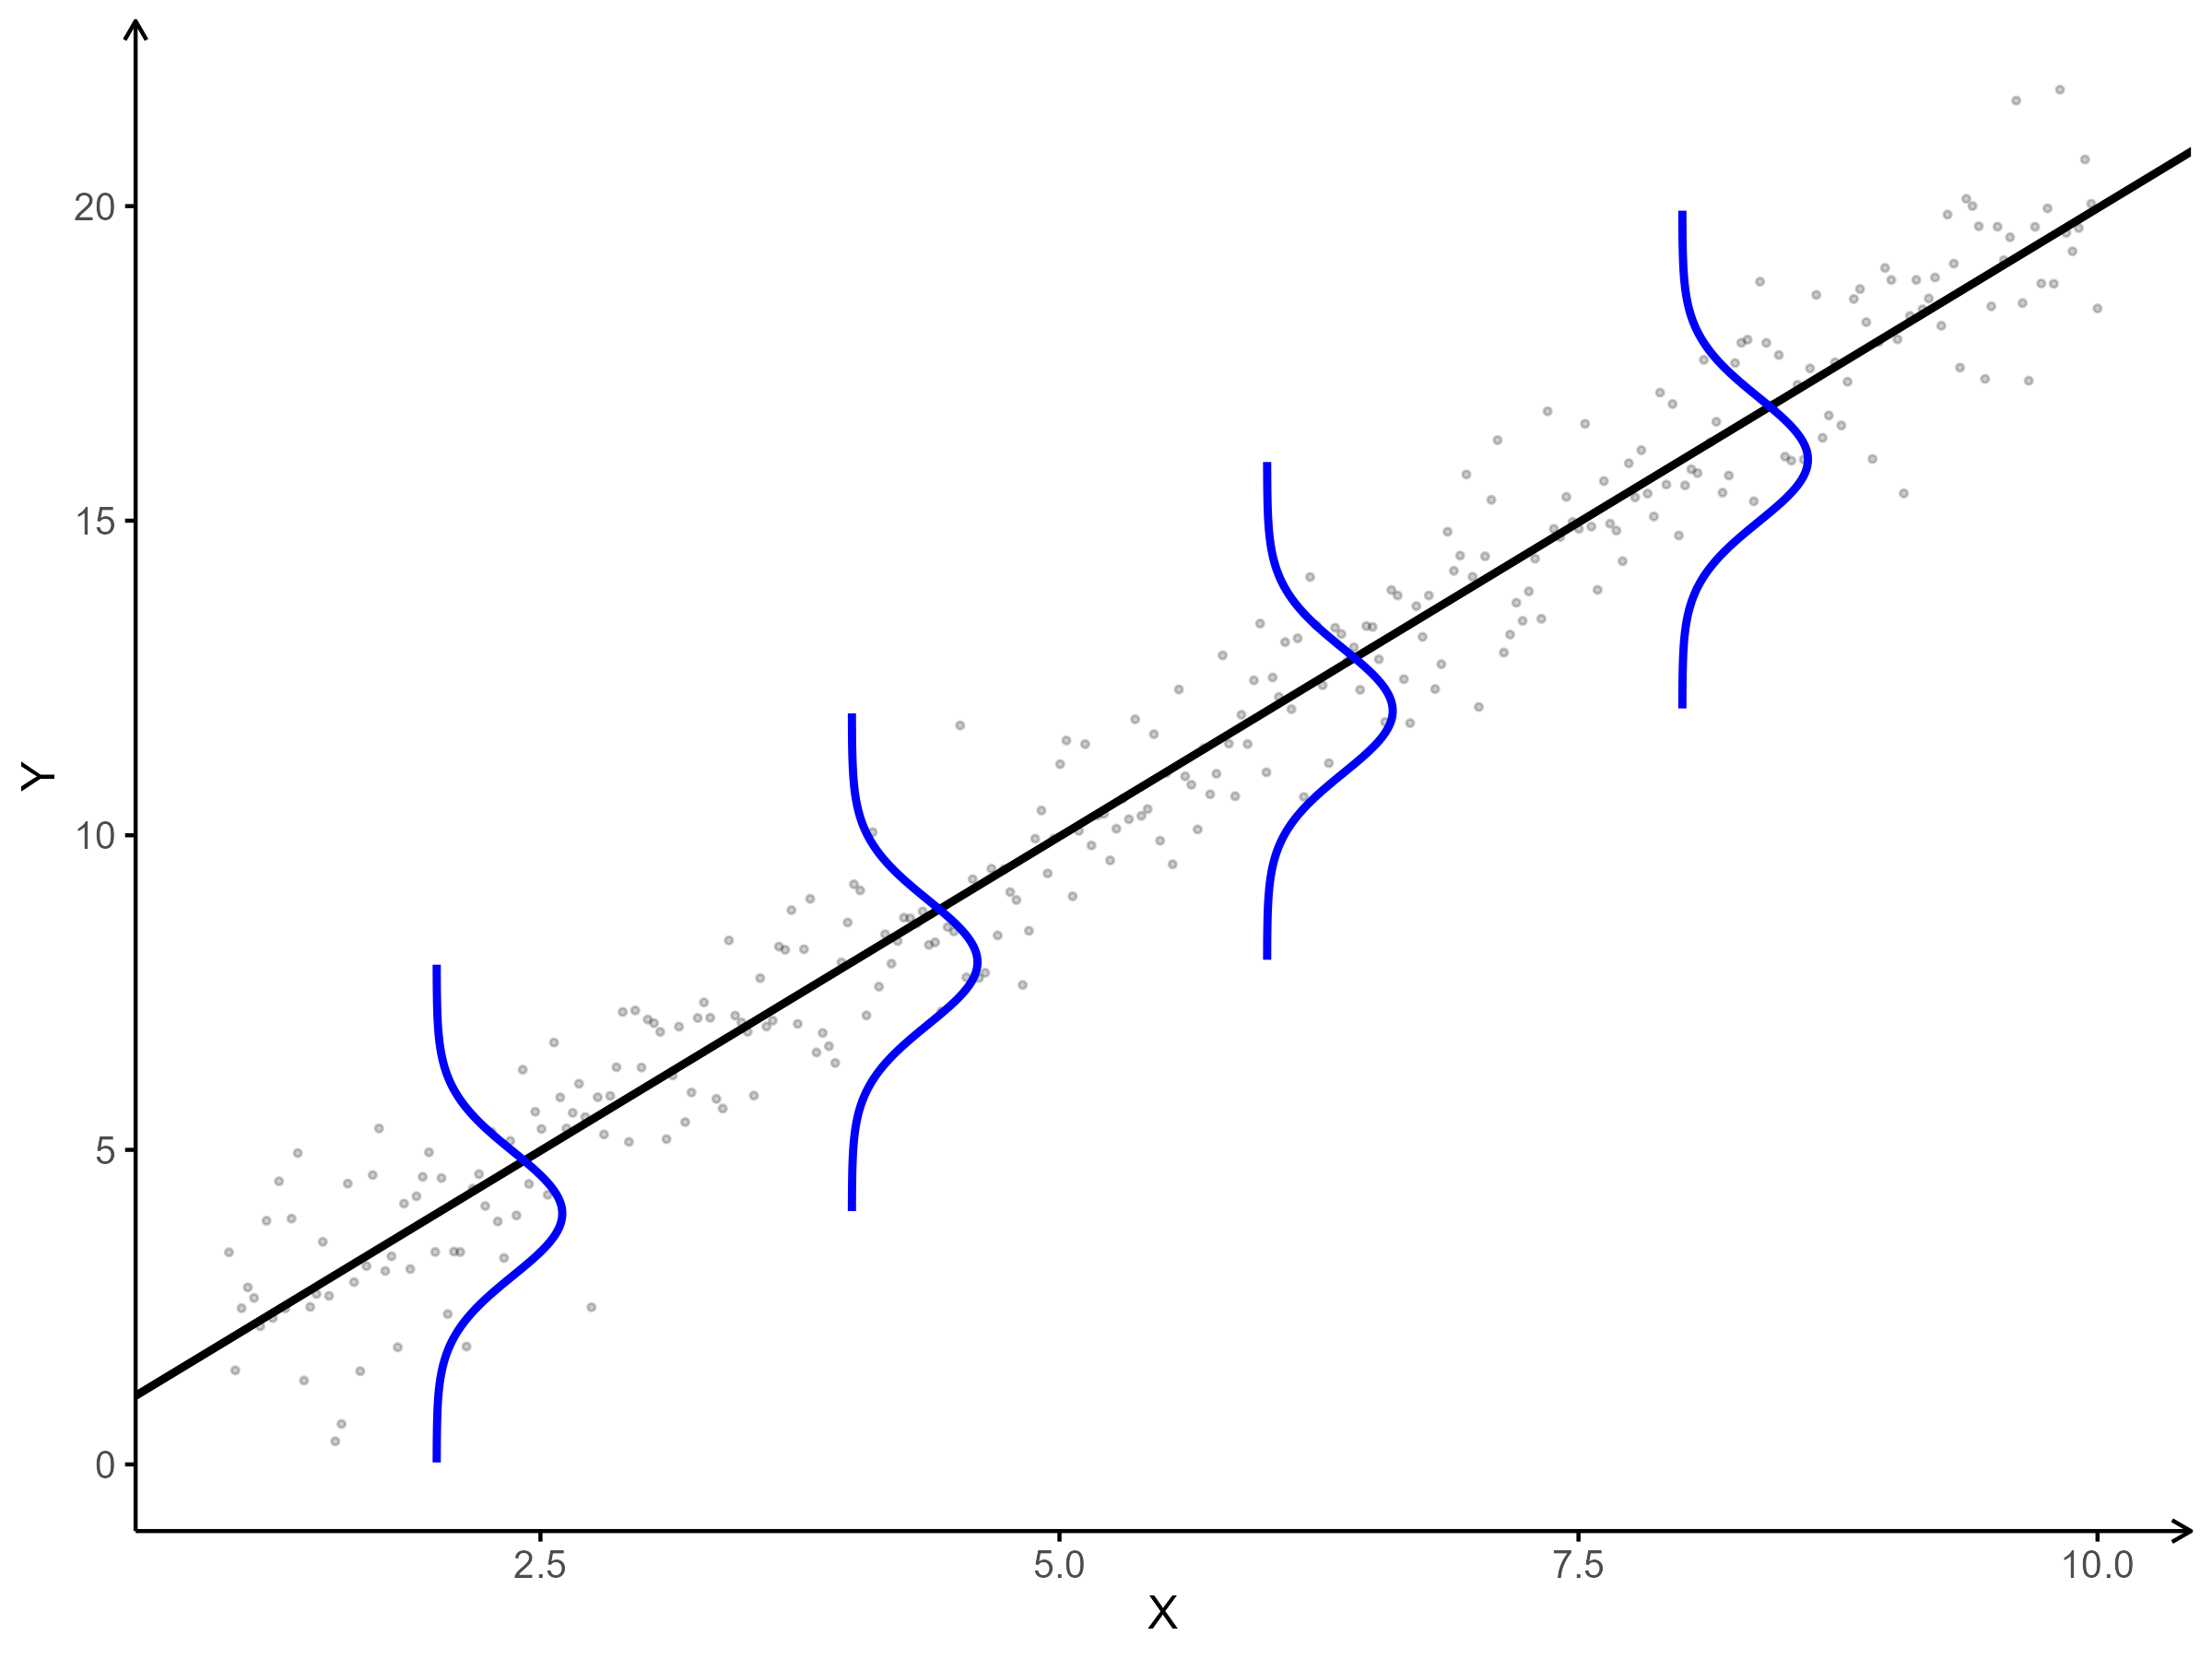
\includegraphics[width=\textwidth]{img/conditional_distributions.png}
\end{column}
\end{columns}

\vspace{0.3cm}

% Neural Networks
\begin{columns}
\begin{column}{0.75\textwidth}
\textbf{Neural networks:}
\begin{itemize}
    \item E.g. feed-forward NNs, normalizing flows, VACAs
    \item Flexible, but "black-box", data-type limitations
\end{itemize}
\end{column}
\begin{column}{0.23\textwidth}
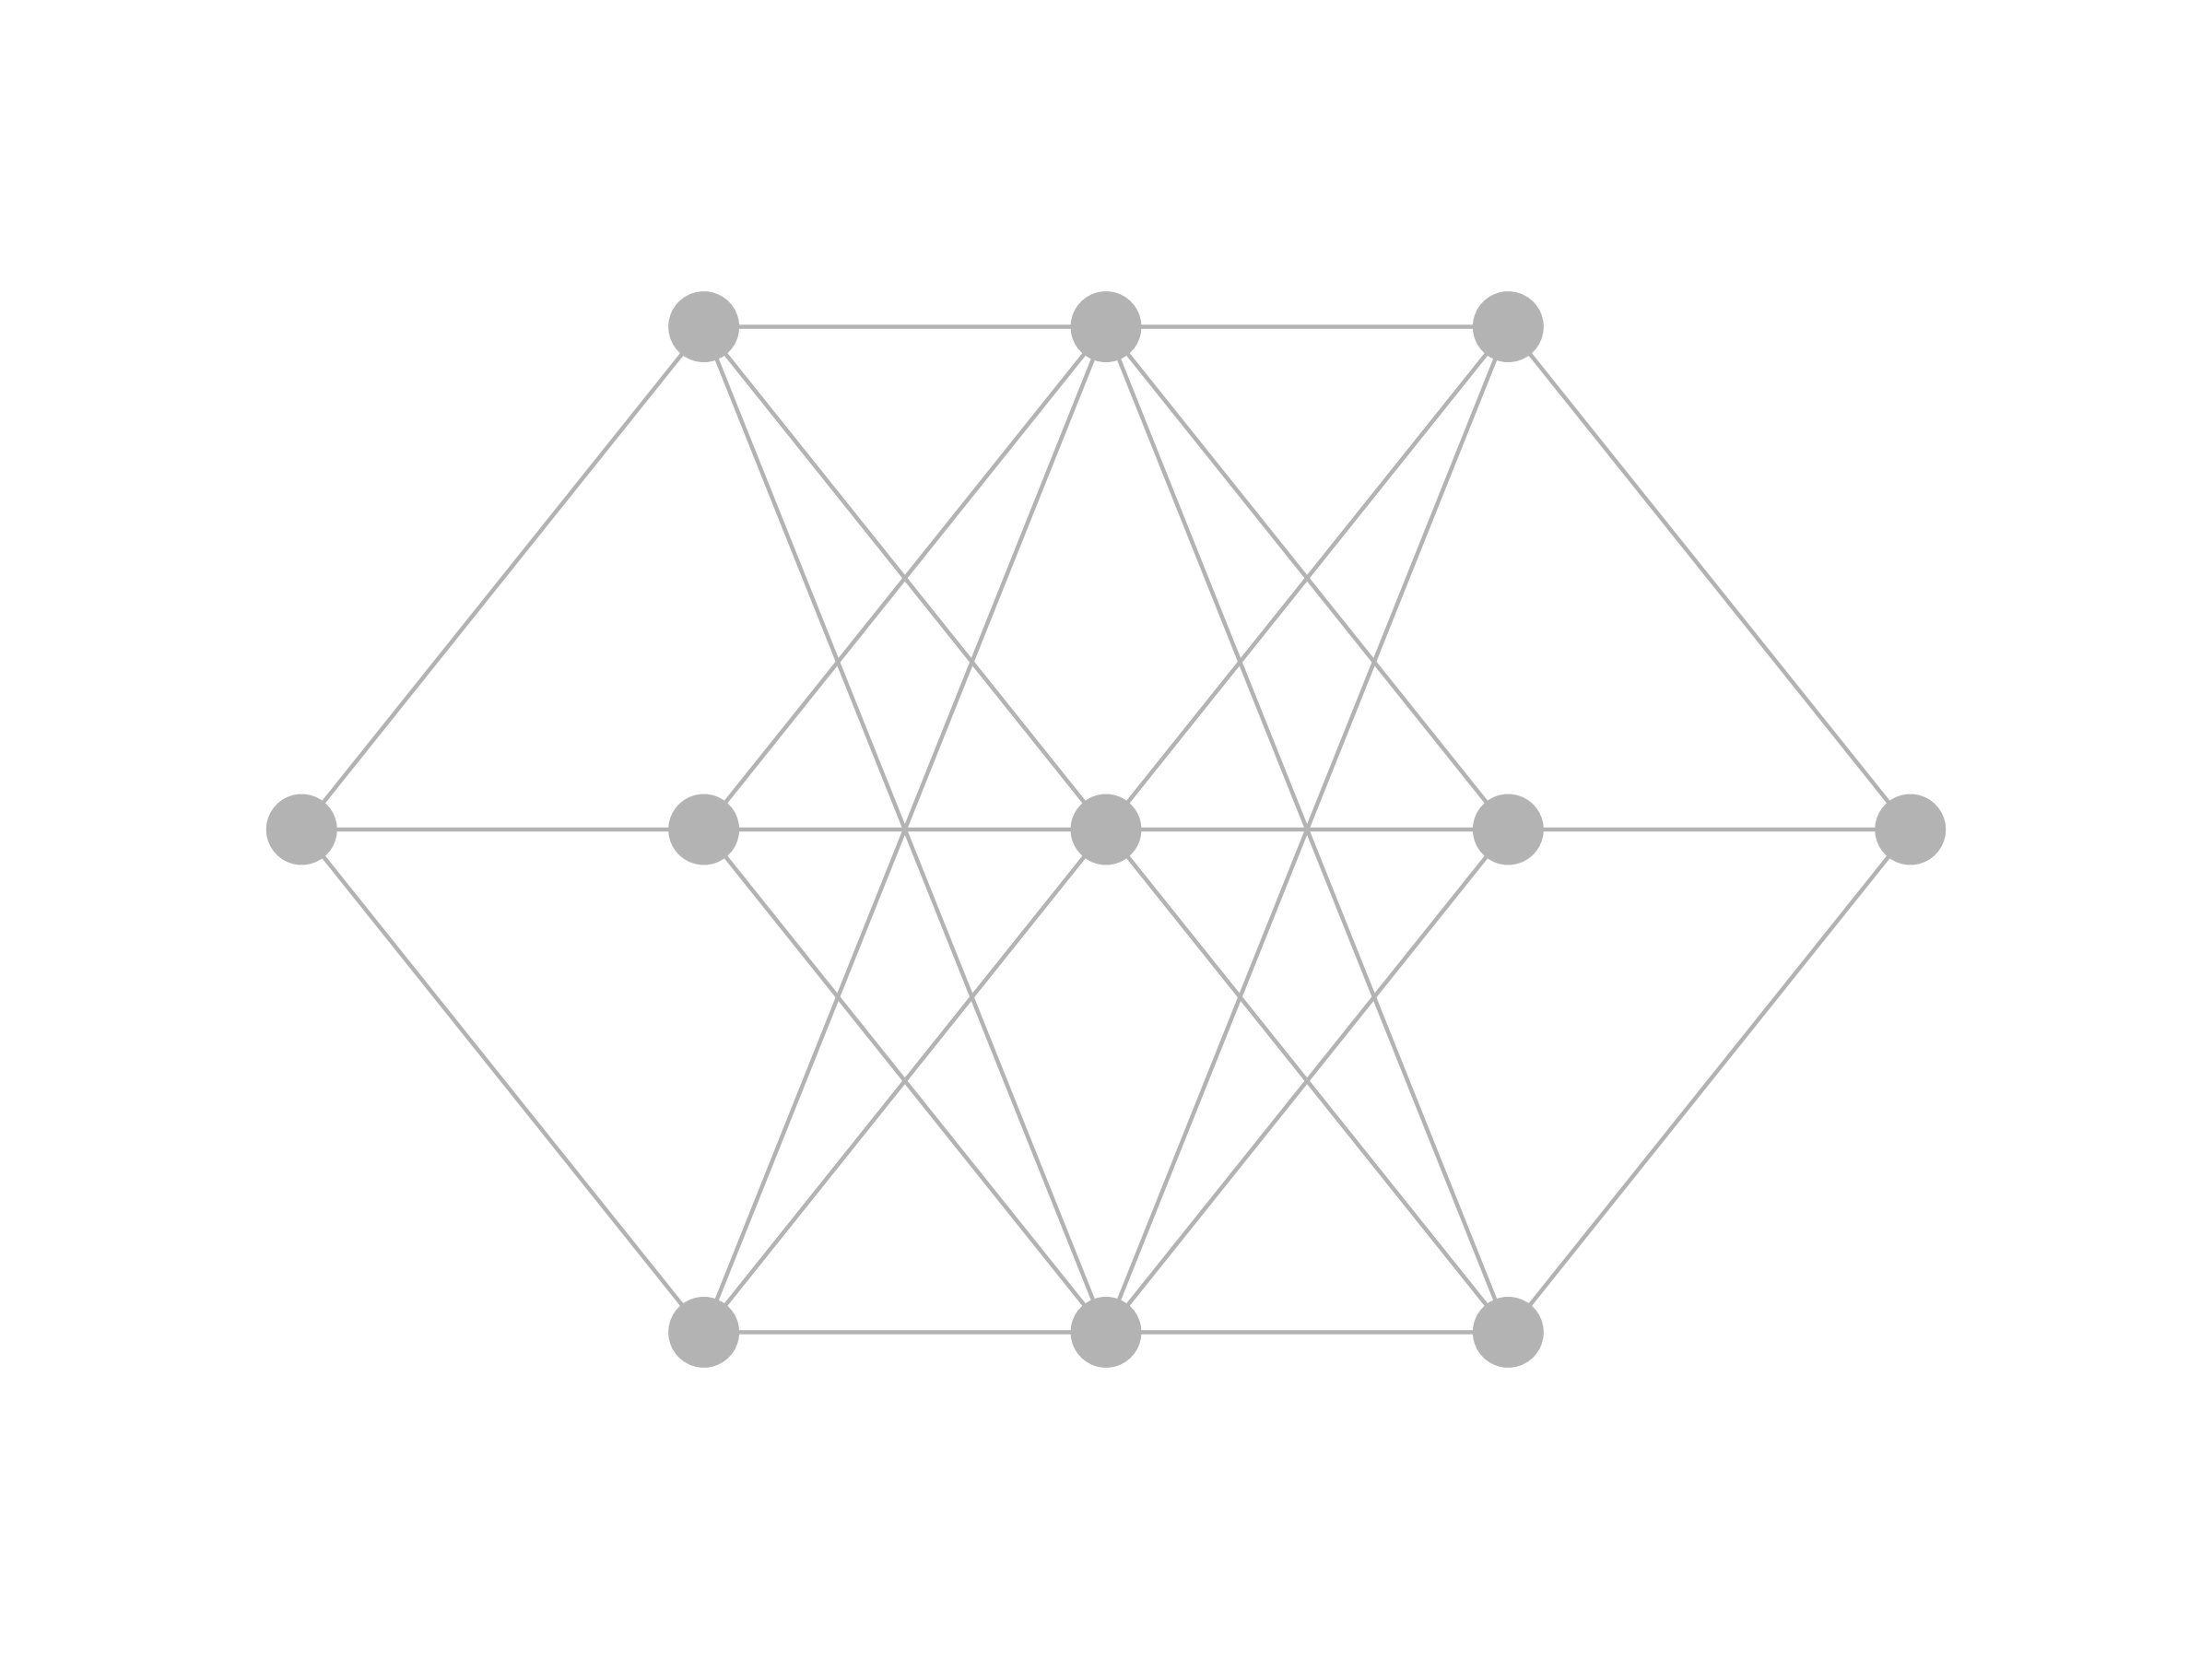
\includegraphics[width=\textwidth]{img/neural_network.png}
\end{column}
\end{columns}

\vspace{0.3cm}

% TRAM-DAGs
\begin{columns}
\begin{column}{0.75\textwidth}
\textbf{TRAM-DAGs:}
\begin{itemize}
    \item Compromise: flexibility + interpretability
    \item Mixed data types
\end{itemize}
\end{column}
\begin{column}{0.23\textwidth}
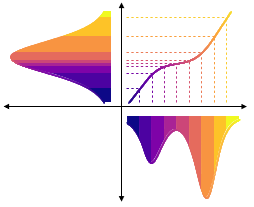
\includegraphics[width=\textwidth]{img/TRAM_Raw.png}
\end{column}
\end{columns}

\end{frame}









\begin{frame}{Transformation Models}

Flexible distributional regression method \citep{hothorn2014}

\vspace{0.4cm}

\textbf{Continuous } $Y \in \mathbb{R}$: 
\[
F_{Y \mid \mathbf{X} = \mathbf{x}}(y) = F_Z(h(y) + \mathbf{x}^\top \boldsymbol{\beta})
\]

\textbf{Discrete } $Y \in \{y_1, y_2, \ldots, y_K\}$: 
\[
P(Y \leq y_k \mid \mathbf{X} = \mathbf{x}) = F_Z(\vartheta_k + \mathbf{x}^\top \boldsymbol{\beta}), \quad k = 1, 2, \ldots, K - 1
\]

\vspace{0.4cm}

\begin{itemize}
    \item $F_Z$: CDF of the standard logistic distribution
    \item $h$: Transformation function, monotonically increasing
    \item $\mathbf{x}$: Predictors
\end{itemize}

\end{frame}






\begin{frame}{Transformation Models}

\begin{columns}

% Left column: Continuous Y
\begin{column}{0.48\textwidth}
\textbf{Continuous $Y$:}

{\small
\vspace{0.2cm}
Intercept: Bernstein polynomial
\vspace{0.2cm}

\scalebox{0.85}{$
h_I(y) = \frac{1}{M + 1} \sum_{k=0}^{M} \vartheta_k \, \text{B}_{k, M}(y)
$}

\vspace{0.2cm}

\scalebox{0.85}{$
h(y \mid \mathbf{x}) = h_I(y) - \mathbf{x}^\top \boldsymbol{\beta}
$}
}

\end{column}

% Right column: Discrete/Ordinal Y
\begin{column}{0.48\textwidth}
\textbf{Discrete/Ordinal $Y$:}

{\small

\vspace{0.2cm}
Intercept: Cut-off value
\vspace{0.2cm}

\scalebox{0.85}{$
h_I(y_k) = \vartheta_k
$}

\vspace{0.2cm}

\scalebox{0.85}{$
h(y_k \mid \mathbf{x}) = h_I(y_k) - \mathbf{x}^\top \boldsymbol{\beta}
$}
}

\end{column}

\end{columns}

\vspace{0.3cm}
\centering
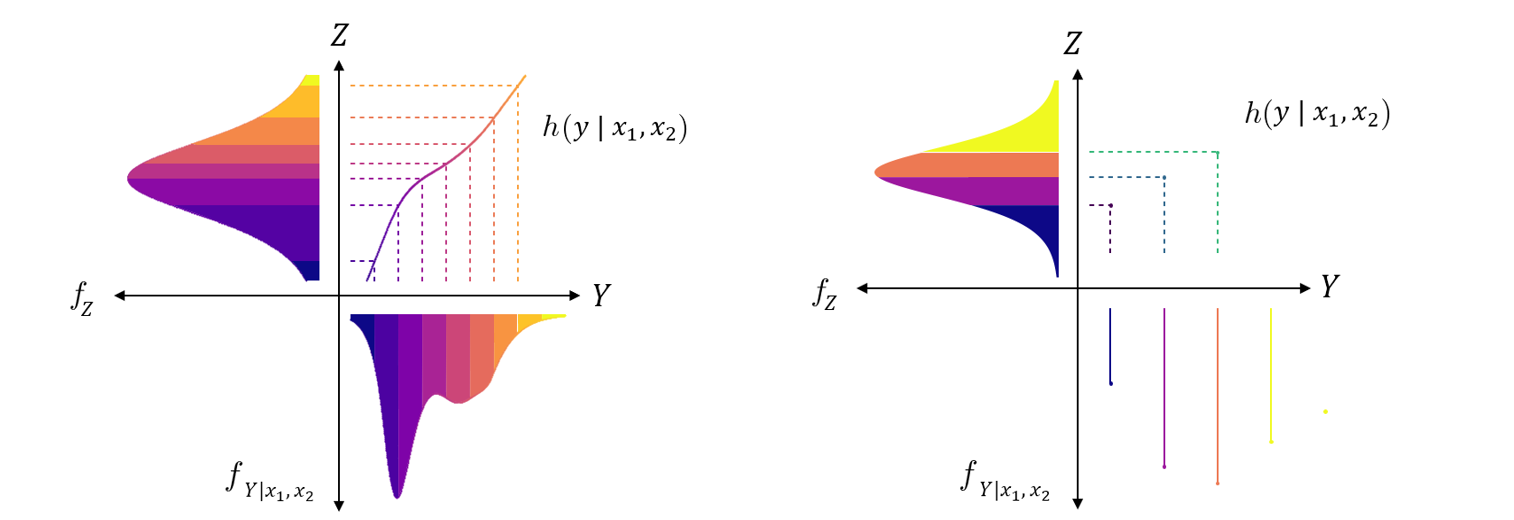
\includegraphics[width=0.9\textwidth]{img/TRAM_Cont_Ord.png}

\end{frame}








\begin{frame}{Deep TRAMs}
  \begin{itemize}
    \item Extended to Deep TRAMs \citep{sick2020}
    \item Flexible components
    \item Minimize the NLL through NN optimization
  \end{itemize}

  \vfill
  \centering
  \includegraphics[width=0.9\linewidth]{img/deep_TRAM.png}
\end{frame}





\begin{frame}{TRAM-DAGs}

  \centering
  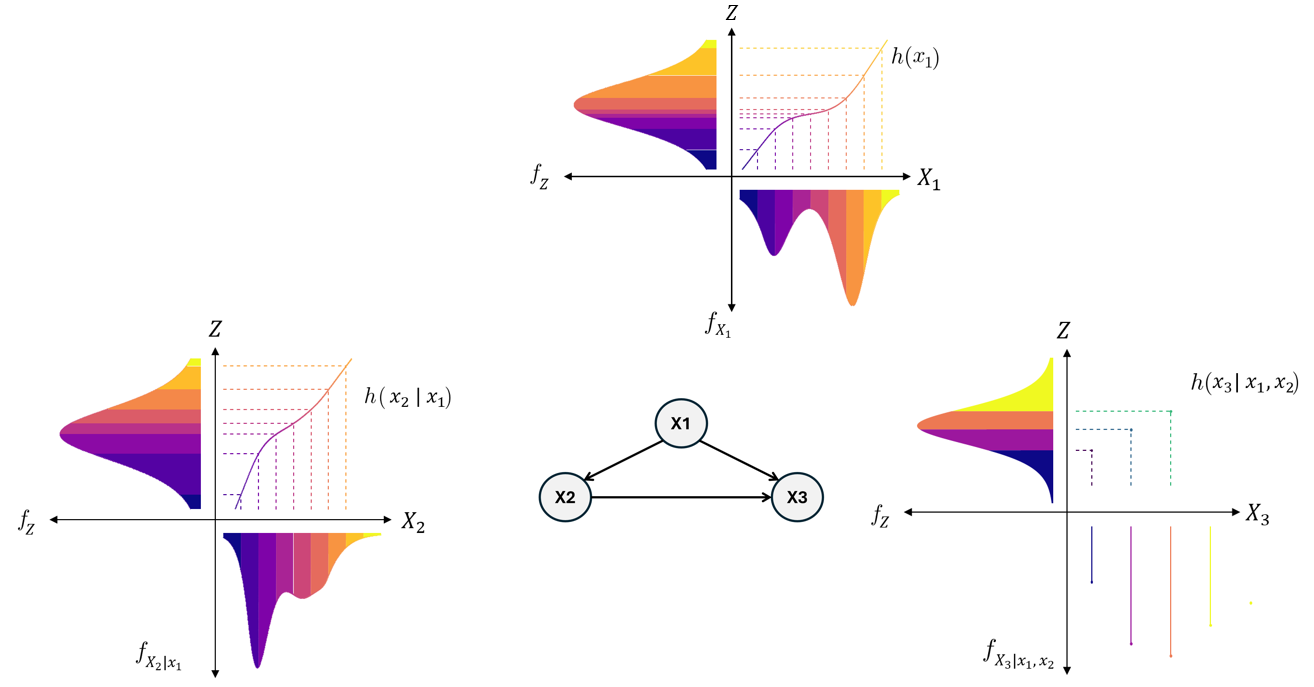
\includegraphics[width=1\linewidth]{img/TRAM_DAG.png}
\end{frame}






\begin{frame}{Simulation Example}
  \begin{itemize}
    \item We have:
    \begin{itemize}
      \item Observational data (simulated)
      \item Predefined DAG
    \end{itemize}
    \item We want:
    \begin{itemize}
      \item Estimate conditional CDF of each variable
      \item Sample from conditional distributions for causal queries with structural equations $x_i = h^{-1}(z_i \mid \text{pa}(x_i))$
    \end{itemize}
  \end{itemize}

  \vfill
  \centering
  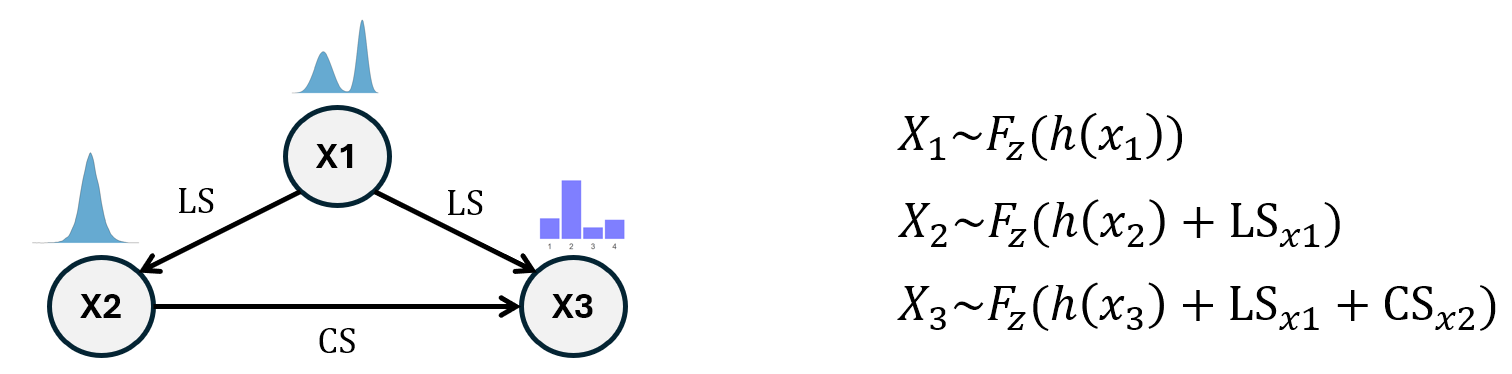
\includegraphics[width=0.7\linewidth]{img/Simulation_Example.png}
\end{frame}



% 
% \begin{frame}{Adjacency Matrix}
% 
% Model structure represented by a meta-adjacency matrix:
% 
% \begin{itemize}
%   \item \textbf{Rows}: source of effect
%   \item \textbf{Columns}: target of effect
% \end{itemize}
% 
% \vspace{0.4cm}
% 
% \begin{center}
% \begin{tikzpicture}[baseline={(current bounding box.center)}]
% 
%   % DAG image
%   \node (img) at (0, 0) {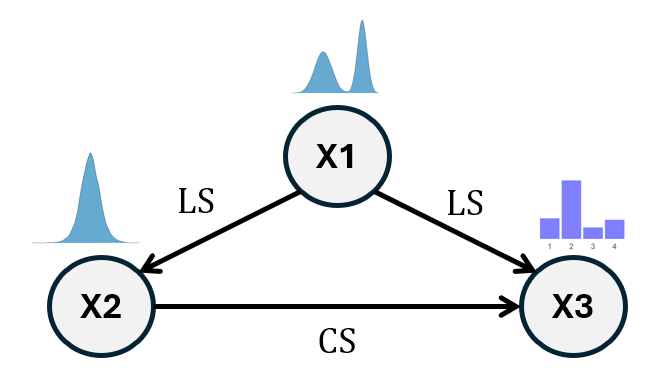
\includegraphics[width=0.28\textwidth]{img/DAG_MA.png}};
% 
%   % Matrix
%   \node (matrix) at (5, 0) {
%     $\mathbf{MA} =
%     \begin{bmatrix}
%       0 & \text{LS} & \text{LS} \\
%       0 & 0  & \text{CS} \\
%       0 & 0  & 0
%     \end{bmatrix}$
%   };
% 
%   % Arrow
%   \draw[->, thick] (img.east) -- (matrix.west);
% 
% \end{tikzpicture}
% \end{center}
% 
% \end{frame}



\begin{frame}{Data Generating Process (DGP)}

\begin{columns}

% Left column: Descriptions and formulas
\begin{column}{0.72\textwidth}

\textbf{\(X_1\):} Continuous, bimodal. \textit{Source node} (independent).

\vspace{0.4cm}

\textbf{\(X_2\):} Continuous. Depends on \(X_1\) (\textcolor{red}{linear}):

\vspace{0.15cm}
{\scriptsize
\[
\textcolor{red}{\beta_{12} = 2}, \quad h_I(X_2) = 5 X_2
\]
\[
\boxed{
h(X_2 \mid X_1) = h_I(X_2) + \textcolor{red}{\beta_{12}} X_1
}
\]
}

\vspace{0.4cm}

\textbf{\(X_3\):} Ordinal. Depends on \(X_1\) (\textcolor{red}{linear}) and \(X_2\) (\textcolor{blue}{complex}):

\vspace{0.15cm}
{\scriptsize
\[
\textcolor{red}{\beta_{13} = 0.2}, \quad \textcolor{blue}{f(X_2) = 0.5 \cdot \exp(X_2)}, \quad \vartheta_k \in \{-2,\, 0.42,\, 1.02\}
\]
\[
\boxed{
h(X_{3,k} \mid X_1, X_2) = \vartheta_k + \textcolor{red}{\beta_{13}} X_1 + \textcolor{blue}{f(X_2)}
}
\]
}


\end{column}

% Right column: Plot
\begin{column}{0.28\textwidth}
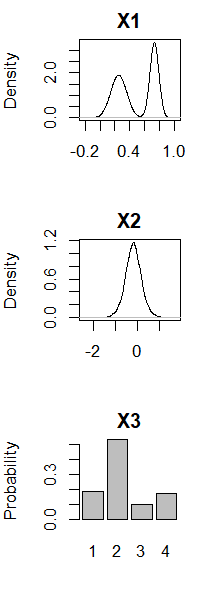
\includegraphics[width=0.8\linewidth]{img/DGP_Variables.png}
\end{column}

\end{columns}

\end{frame}





% \textbf{Parameters:} 281 total (not all used)
% \begin{itemize}
%     \item Simple Intercepts (SI): \textbf{240} \\
%     - only 43 needed (20 + 20 + 3)
%     \item Linear Shifts (LS): \textbf{9} \\
%     - 2 active
%     \item Complex Shifts (CS): \textbf{32} \\
%     - 24 active
% \end{itemize}

% 
% \begin{frame}{Construct Model: Modular Neural Network}
% 
% \begin{columns}
% 
% % Left side: Text
% \begin{column}{0.65\textwidth}
% 
% \vspace{0.1cm}
% 
% \textbf{Inputs:} \\ Observations + adjacency matrix
% 
% \vspace{0.4cm}
% 
% \textbf{Outputs:}
% \begin{itemize}
%     \item Simple Intercepts (SI): \vartheta
%     \item Linear Shifts (LS): $\beta_{12}X_1, \beta_{13}X_2$
%     \item Complex Shift (CS):  $\beta(X_2)$
% \end{itemize}
% 
% 
% 
% \vspace{0.4cm}
% \textbf{Transformation Functions:} \\
% \begin{align*}
% h(X \mid pa(X)) = \text{SI} + \text{LS} + \text{CS} \\
% & h(X_1) = h_I(X_1) \\
% & h(X_2 \mid X_1) = h_I(X_2) + \textcolor{red}{\beta_{12} X_1} \\
% & h(X_{3,k} \mid X_1, X_2) = \vartheta_k + \textcolor{red}{\beta_{13} X_1} + \textcolor{blue}{\beta(X_2)} 
% % \quad \( h = \text{SI} + \text{LS} + \text{CS} \)
% \end{align*}
% \end{column}
% 
% % Right side: Image
% \begin{column}{0.35\textwidth}
% \begin{figure}
%   \centering
%   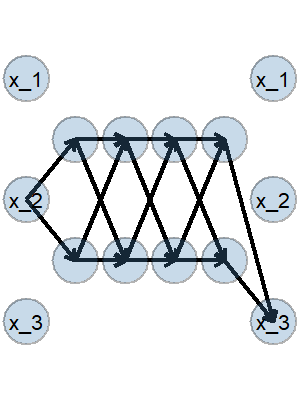
\includegraphics[width=0.65\linewidth]{img/CS.png}
%   \caption{$\text{CS}_{X_2}$ on $X_3$}
% \end{figure}
% 
% \end{column}
% 
% \end{columns}
% 
% \end{frame}
% 


\begin{frame}{Construct Model: Modular Neural Network}

\begin{columns}

% Left side: Text
\begin{column}{0.65\textwidth}

\vspace{0.1cm}

\textbf{Inputs:} \\ Observations + assumed structure

\vspace{0.4cm}

\textbf{Outputs:}
\begin{itemize}
    \item Simple Intercepts (SI): $\textcolor{violet}{\vartheta}$
    \item Linear Shifts (LS): $\textcolor{red}{\beta_{12}X_1}, \textcolor{red}{\beta_{13}X_2}$
    \item Complex Shift (CS):  $\textcolor{blue}{f(X_2)}$
\end{itemize}

\vspace{0.4cm}
\textbf{Transformation Functions:}
\begin{align*}
& \boxed{h(X_i \mid pa(X_i)) = \text{SI} + \text{LS} + \text{CS}} \\
& h(X_1) = \textcolor{violet}{h_I(X_1)} \\
& h(X_2 \mid X_1) = \textcolor{violet}{h_I(X_2)} + \textcolor{red}{\beta_{12} X_1} \\
& h(X_{3,k} \mid X_1, X_2) = \textcolor{violet}{\vartheta_k} + \textcolor{red}{\beta_{13} X_1} + \textcolor{blue}{f(X_2)} 
\end{align*}

\end{column}

% Right side: Image
\begin{column}{0.35\textwidth}
\begin{figure}
  \centering
  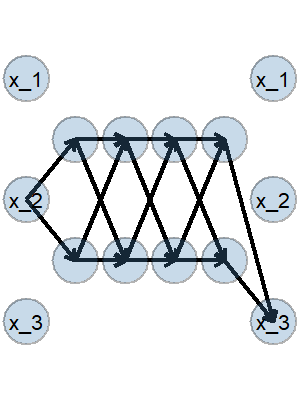
\includegraphics[width=0.65\linewidth]{img/CS.png}
  \caption{$\text{CS}_{X_2}$ on $X_3$}
\end{figure}
\end{column}

\end{columns}

\end{frame}


% \begin{frame}{Experiment 1: TRAM-DAGs}
% \begin{itemize}
%         \item Samples: 20'000 training observations
%         \item Learning rate: 0.005
%         \item Epochs: 400
%         \item Minimizing negative log likelihood (NLL) during training
%         
% \end{itemize}
% \end{frame}


\begin{frame}{Experiment 1: TRAM-DAGs (model learning)}

% no centering

20,000 training samples
{
\centering
  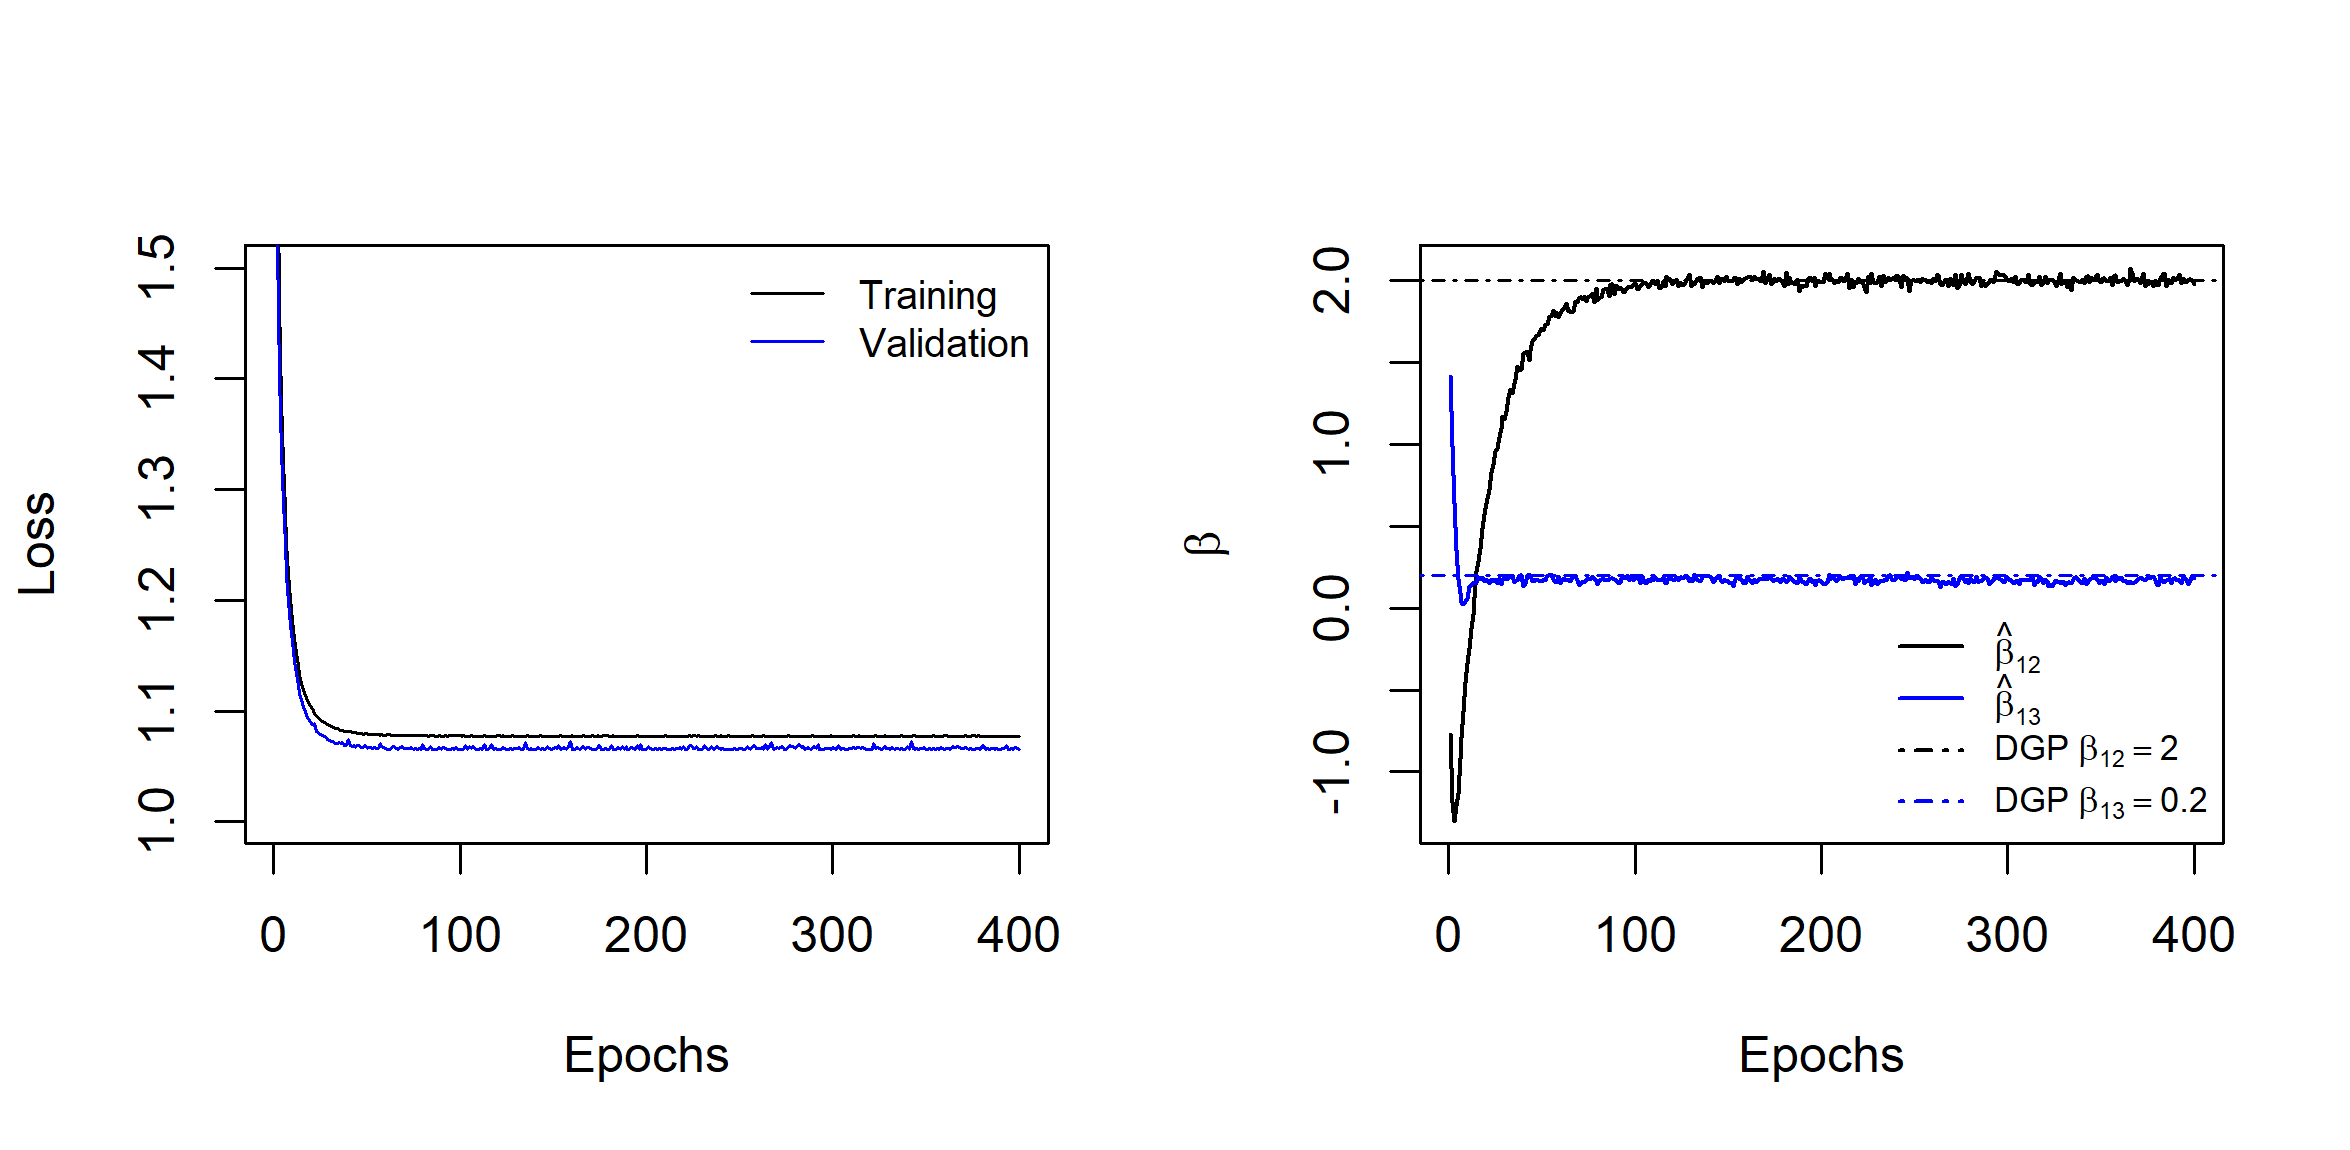
\includegraphics[width=1\linewidth]{img/experiment1/exp1_loss_parameters.png}
}
  


\end{frame}



\begin{frame}{Sampling from the Fitted TRAM-DAG (observational)}

\begin{columns}

% Left column: Sampling explanation
\begin{column}{0.65\textwidth}

\textbf{Nodes $X_i , i \in \{1,\, 2,\, 3\}$:}

\vspace{0.2cm}

\begin{itemize}
    \item Sample latent value: 
    \[
    z_i \sim F_{Z_i} \quad \text{(e.g., \texttt{rlogis()} in R)}
    \]

    \item Determine \(x_i\) such that:

    \begin{itemize}
        \item \textbf{If \(X_i\) is continuous:}
        Solve for \(x_i\) using numerical root-finding:
        \[
        h(x_i \mid \text{pa}(x_i)) - z_i = 0
        \]
        % \[
        % h(x_i \mid \text{pa}(x_i)) - z_i = 0 \text{ for } x_i \text{ (numerical root-finding)}
        % \]
        % 
        \item \textbf{If \(X_i\) is ordinal:}
        find the smallest category $x_i$ such that
        \[
        x_i = \max \left( \{0\} \cup \left\{ x : z_i > h(x \mid \text{pa}(x_i)) \right\} \right) + 1
        \]
        
    \end{itemize}
\end{itemize}

\end{column}

% Right column: Illustration
\begin{column}{0.3\textwidth}
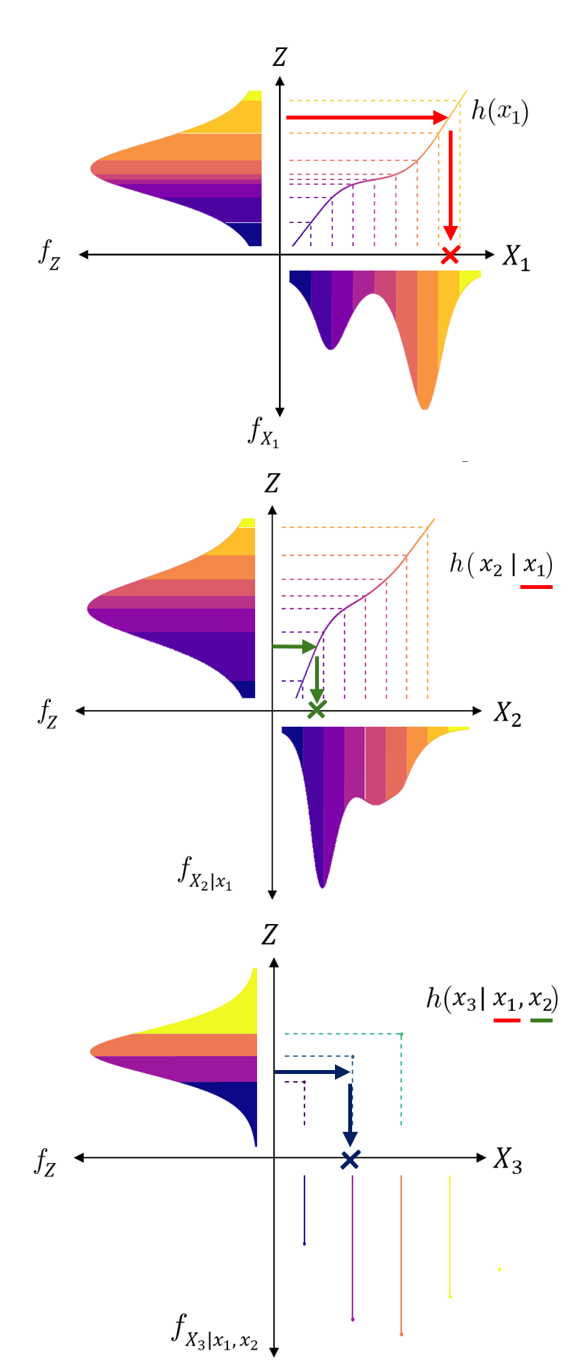
\includegraphics[width=0.9\linewidth]{img/Sampling.png}
\end{column}

\end{columns}

\end{frame}




\begin{frame}{Sampling from the Fitted TRAM-DAG (interventional)}

\textbf{Interventional sampling:} \\

\begin{itemize}
    \item Do-intervention: \( \textcolor{red}{\text{do}(x_2 = \alpha})\)
    \item Sample from the interventional-distribution:
\end{itemize}
\[
x_3 = \min \left\{ x : z_3 \le h(x \mid x_1, \textcolor{red}{x_2 = \alpha}) \right\}
\]

\centering
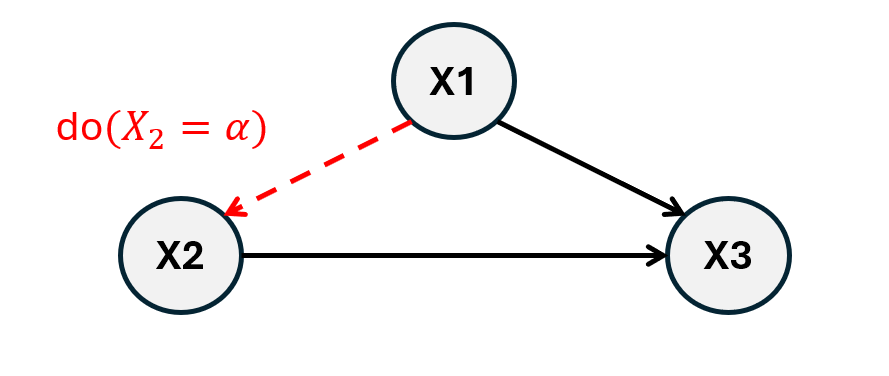
\includegraphics[width=0.5\linewidth]{img/interventional.png}


\end{frame}



\begin{frame}{Experiment 1: TRAM-DAGs (sampling distributions)}

  \centering
  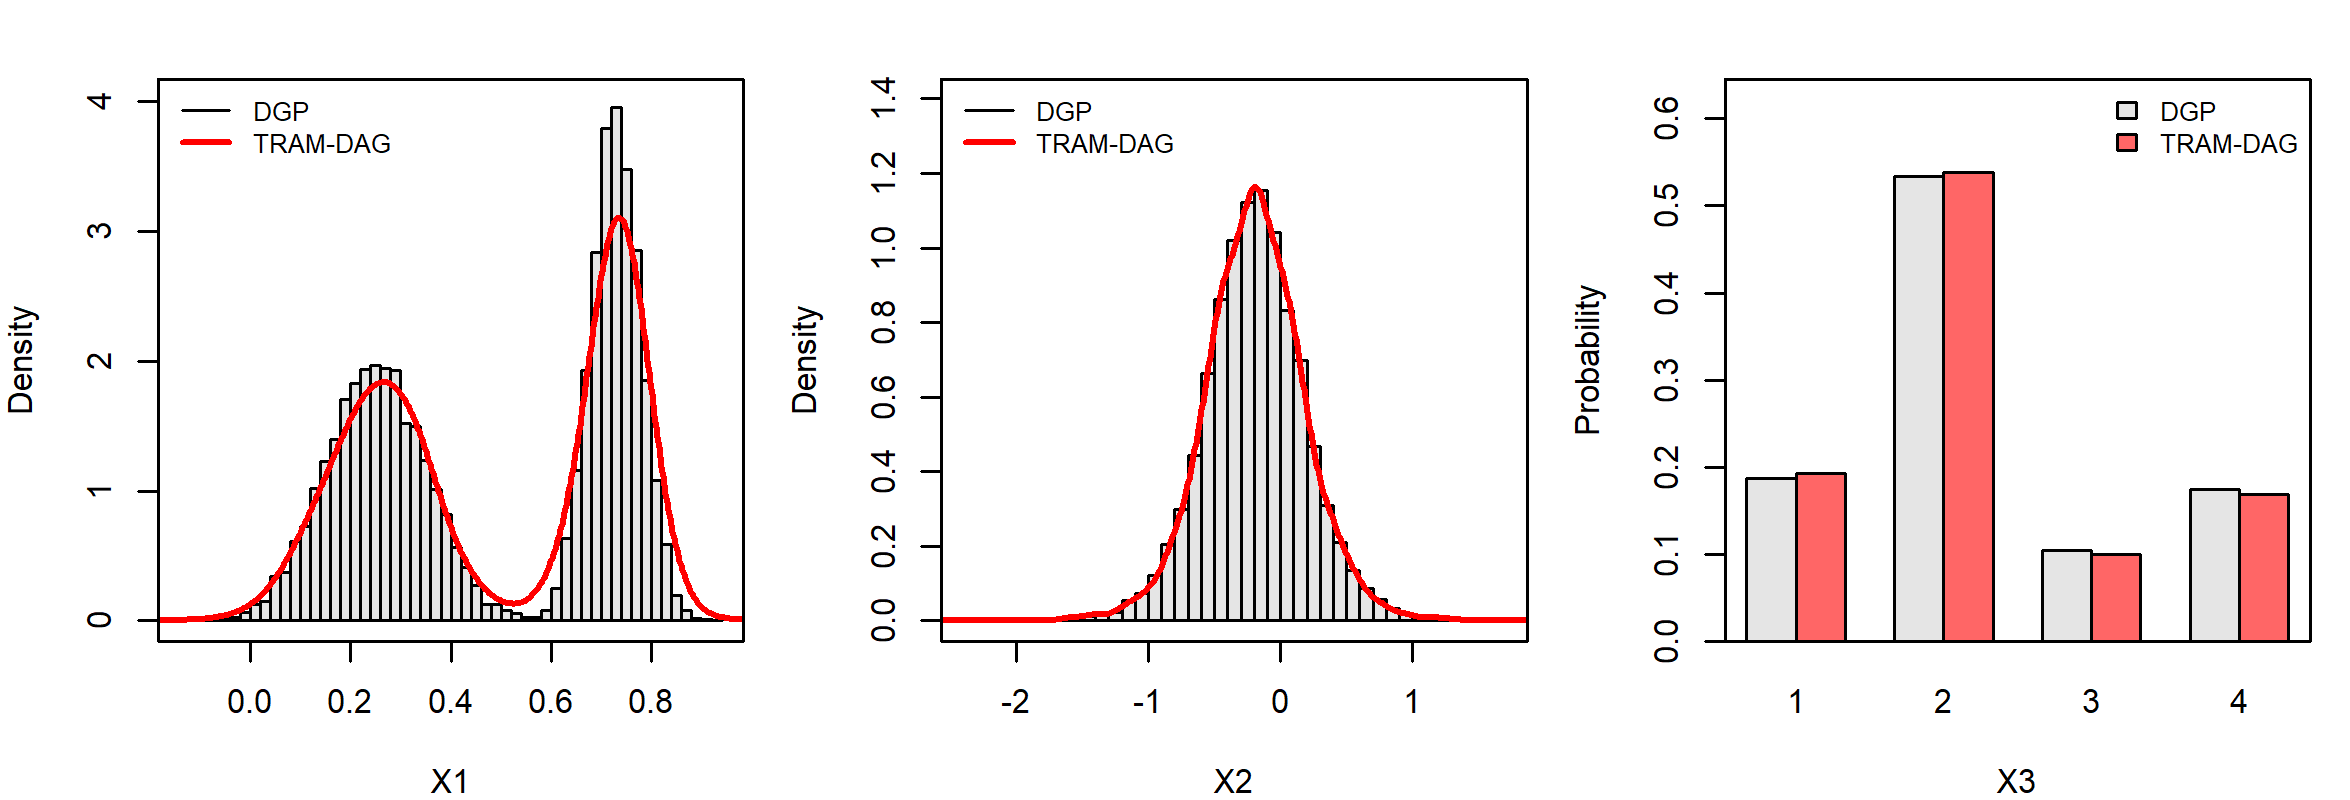
\includegraphics[width=0.9\linewidth]{img/experiment1/exp1_observational_distribution.png}
  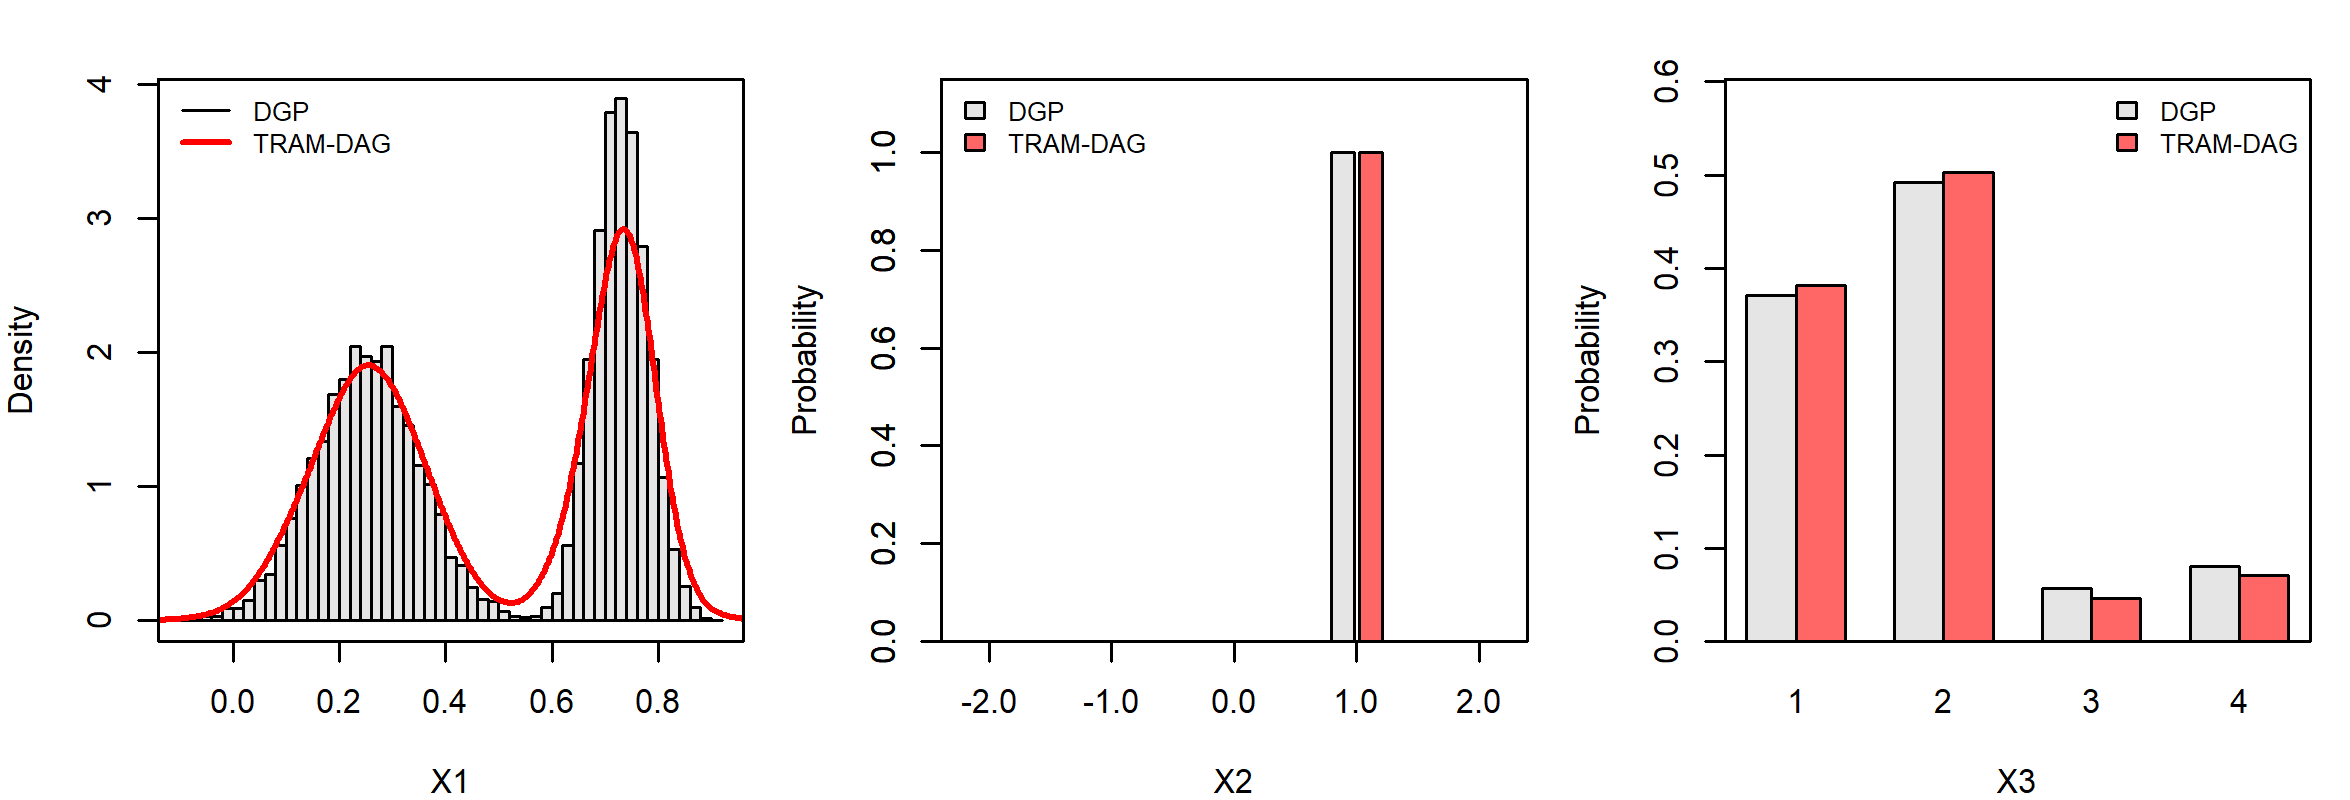
\includegraphics[width=0.9\linewidth]{img/experiment1/exp1_interventional_distribution.png}

\end{frame}

% 
% 
% \begin{frame}{Experiment 1: TRAM-DAGs (learned shifts)}
% 
%   \centering
%   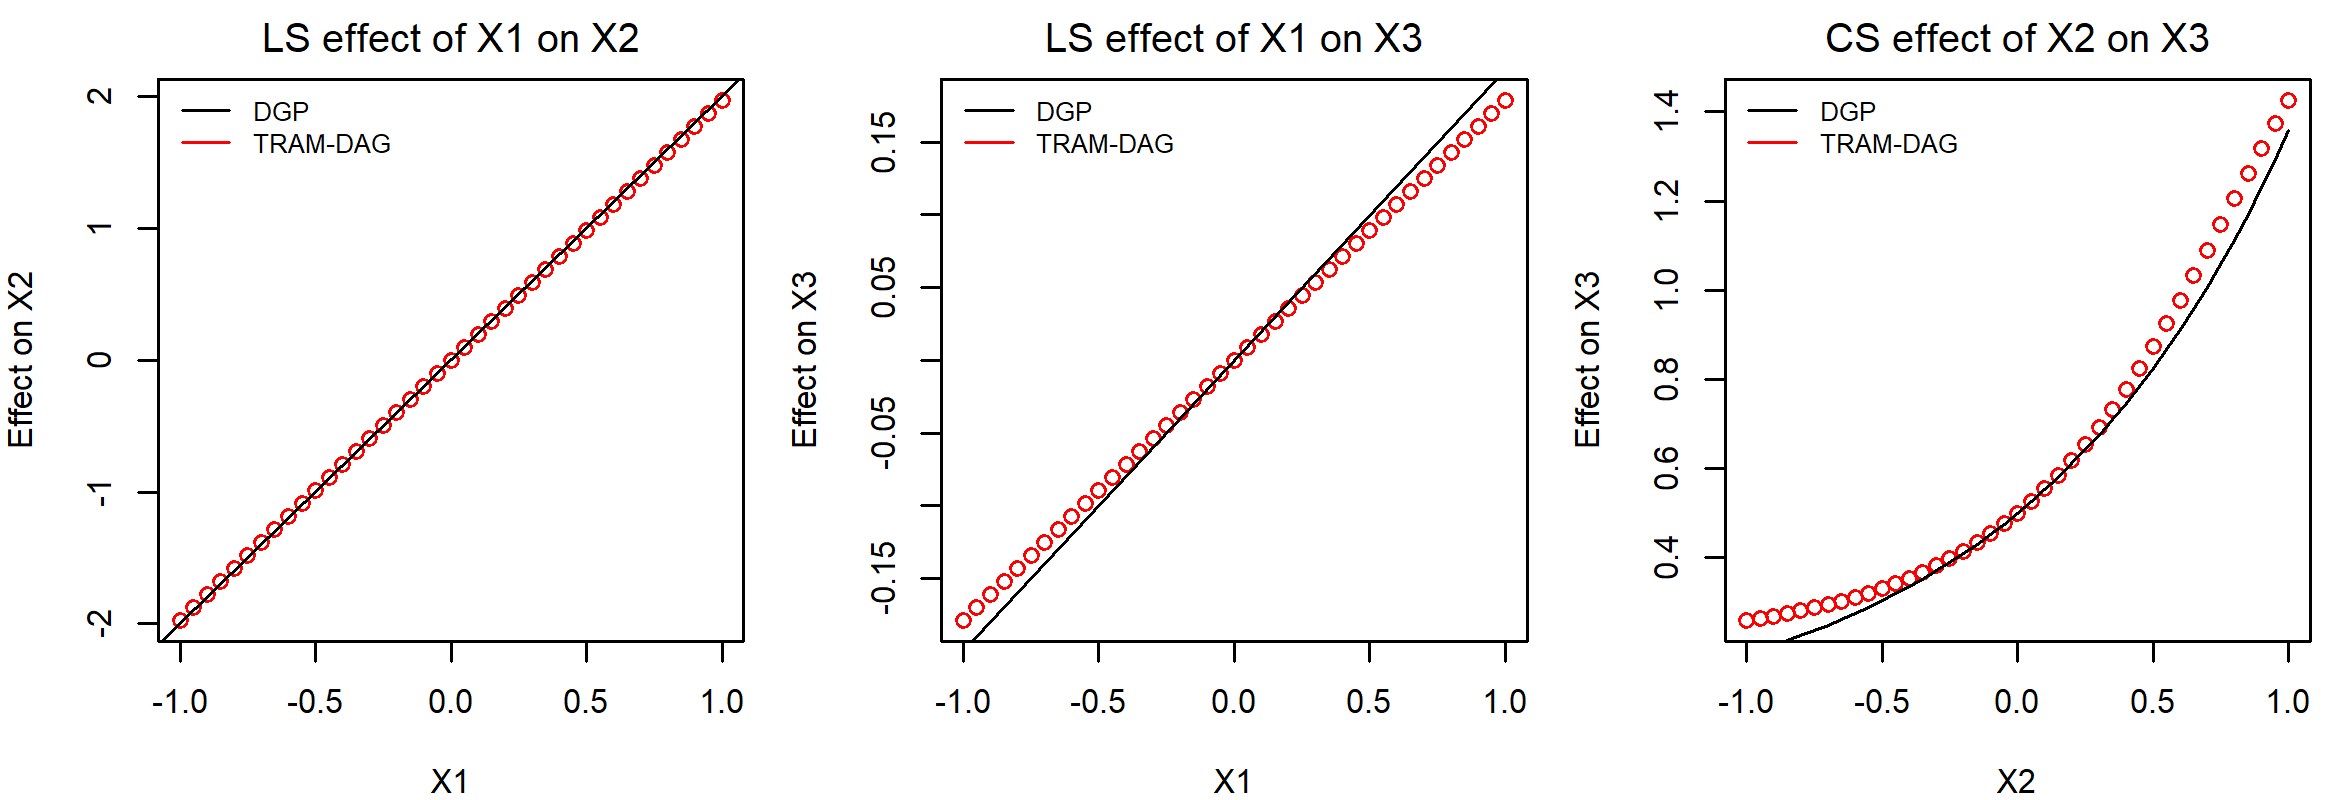
\includegraphics[width=1\linewidth]{img/experiment1/exp1_LS_CS.png}
% 
% \end{frame}
% 
% 
% 
% \begin{frame}{Experiment 1: TRAM-DAGs (learned intercepts)}
% 
%   \centering
%   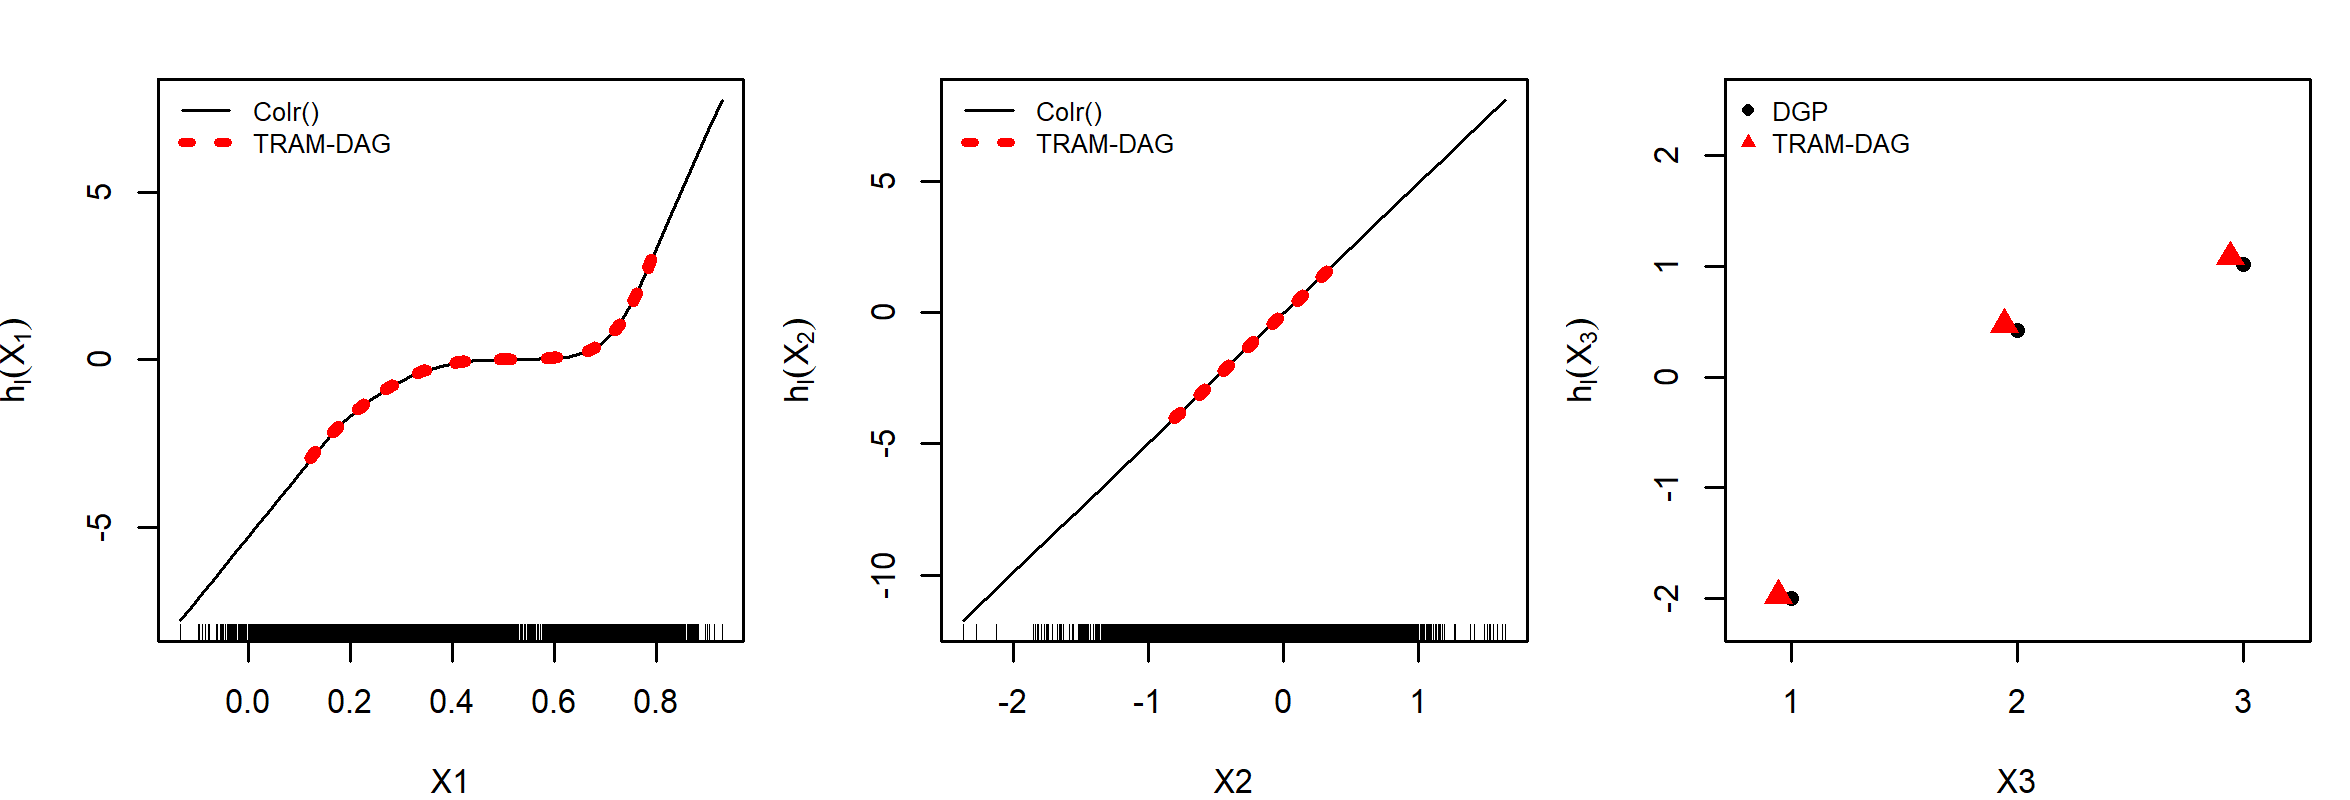
\includegraphics[width=1\linewidth]{img/experiment1/exp1_baseline_trafo.png}
% 
% \end{frame}





\begin{frame}{Experiment 1: TRAM-DAGs (counterfactuals)}

How to determine a counterfactual value for $X_2$, given some observation?

  \centering
  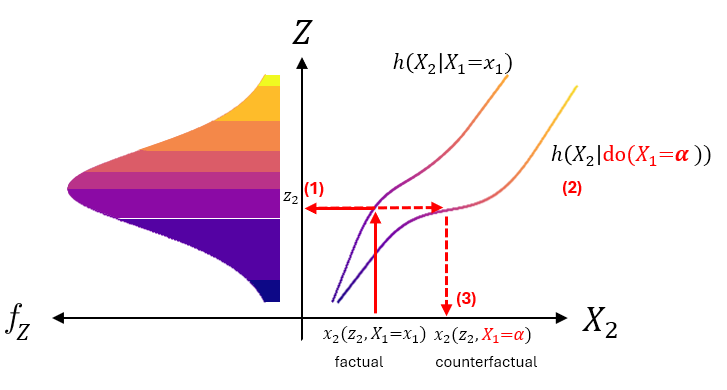
\includegraphics[width=0.95\linewidth]{img/experiment1/counterfactuals.png}

\end{frame}






\begin{frame}{Experiment 1: TRAM-DAGs (counterfactuals)}

\textbf{Counterfactuals:} Counterfactual value of $X_2$ under varying $X_1$

  \centering
  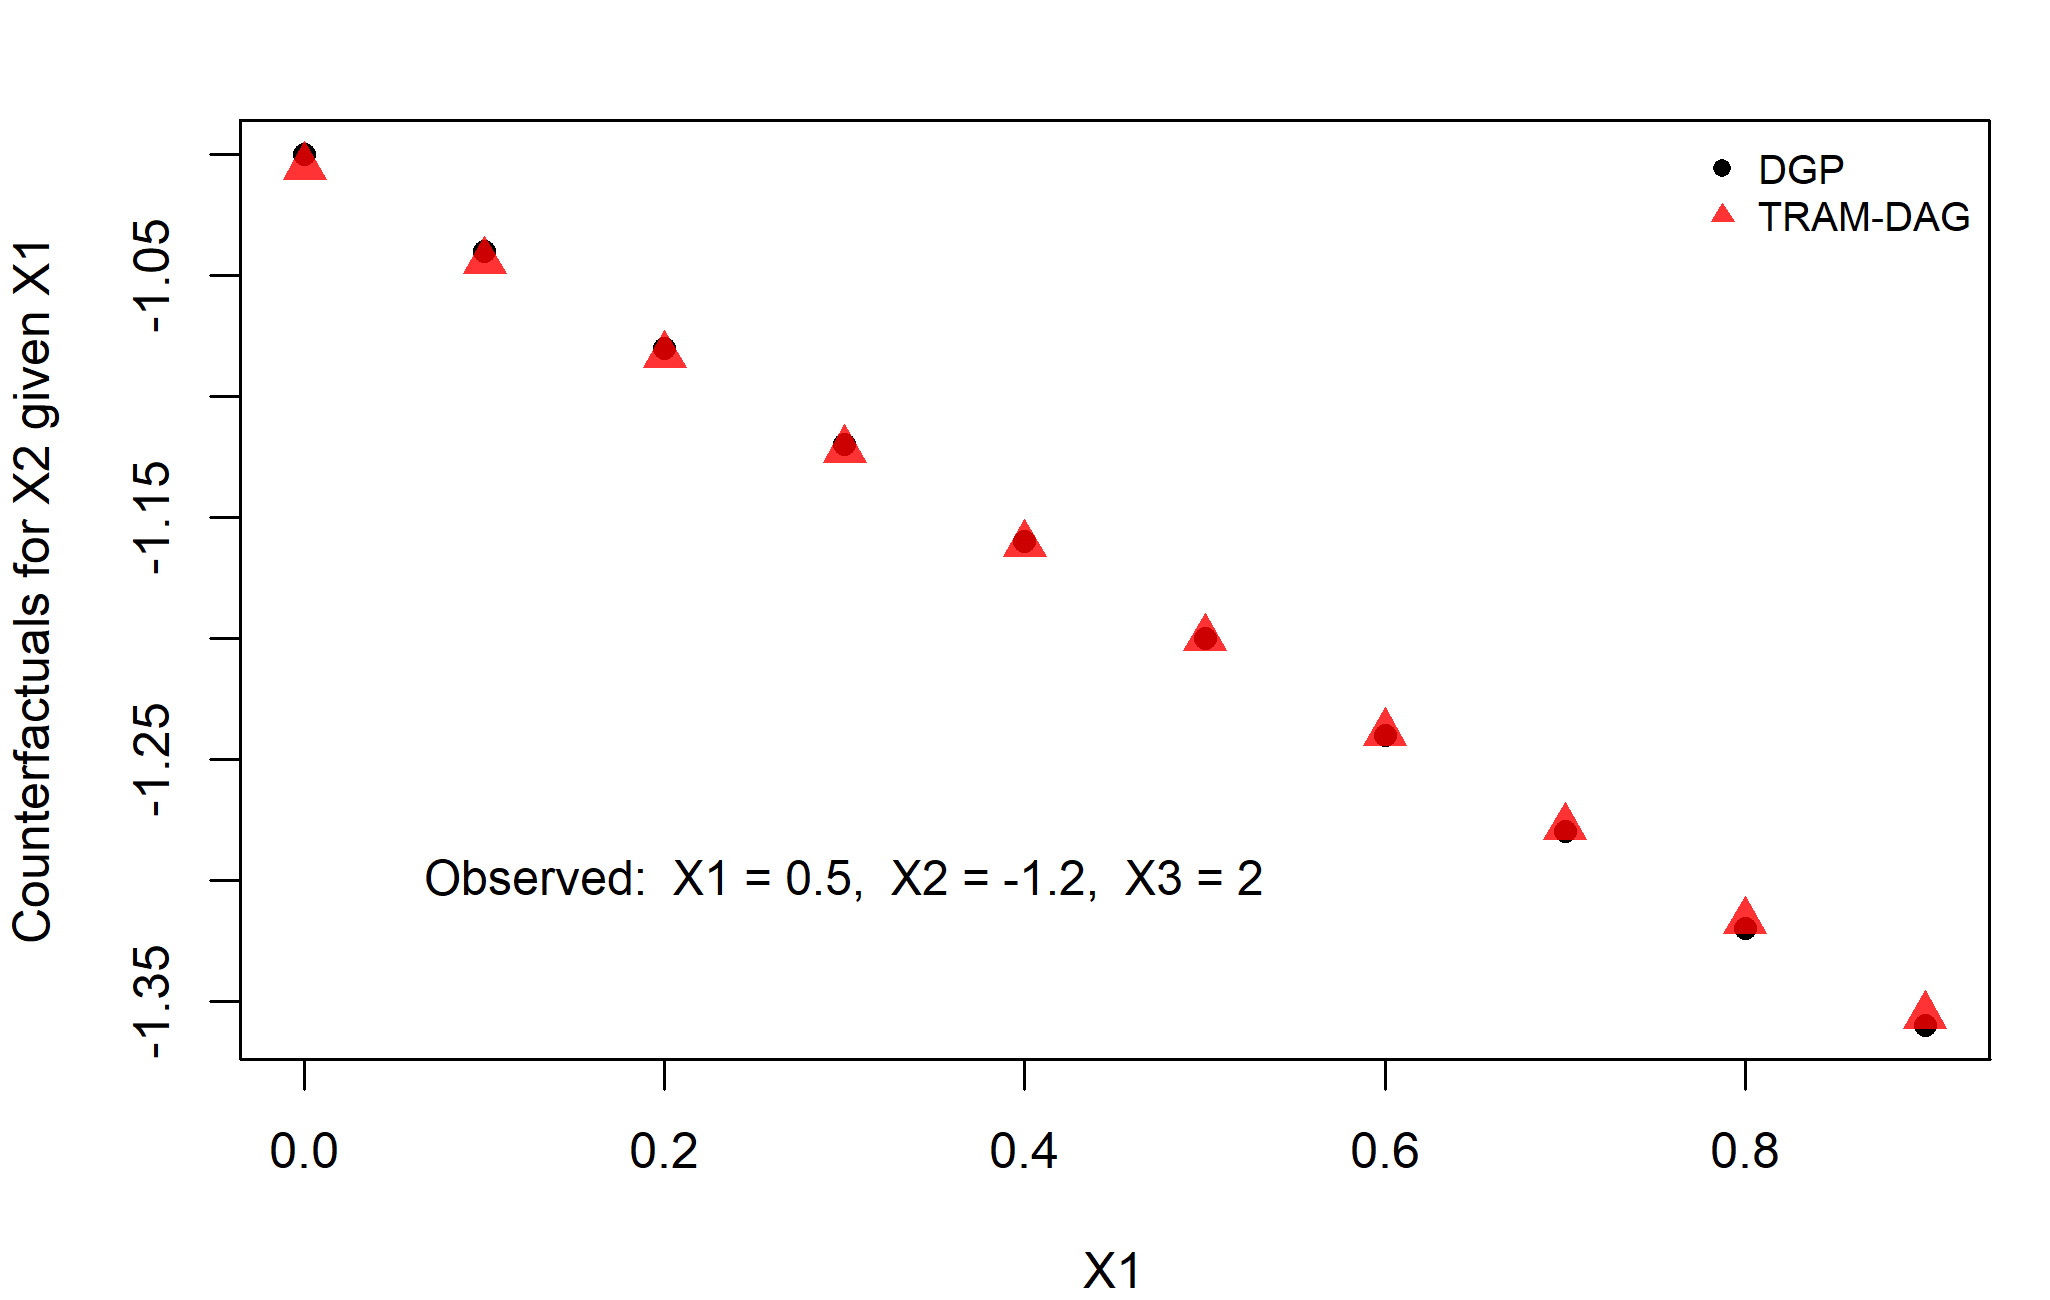
\includegraphics[width=0.9\linewidth]{img/experiment1/exp1_counterfactuals.png}

\end{frame}




\begin{frame}{Experiment 1: TRAM-DAGs (Discussion)}


With TRAM-DAGs we can:

\begin{itemize}
    \item Estimate the functional form of the edges in the DAG
    \item Customize flexibility (SI/CI, LS, CS)
    \item Sample from the fitted model
    \item Estimate counterfactuals
\end{itemize}
\end{frame}








\begin{frame}{Individualized Treatment Effect (ITE): Motivation}


\textbf{Motivation:}

\begin{itemize}
    \item RCT typically estimates Average Treatment Effect (ATE)
    \item Individuals may respond differently depending on characteristics
    \item Crucial for decision-making in personalized medicine or targeted marketing
    \item Heterogeneous treatent effect mainly due to treatment-covariate-interactions
\end{itemize}
    
\textbf{Individual treatment effect:} Difference in potential outcomes

\[
Y_i(1) - Y_i(0)
\]

, where $Y_i(1)$ is the potential outcome if treated and $Y_i(0)$ if not treated.

% arrow Fundamental Problem of Causal Inference:} We cannot observe both potential outcomes for the same individual.

Fundamental problem of causal inference $\rightarrow$ We cannot observe both potential outcomes for the same individual.

\end{frame}



\begin{frame}{Individualized Treatment Effect (ITE): Assumptions}


\textbf{Assumptions for identifiability of causal effects from observed data:}

\begin{enumerate}
    \item \textbf{Consistency:} Observed outcome equals the potential outcome under the treatment actually received: $Y = Y(1)$ if $T = 1$, and $Y = Y(0)$ if $T = 0$
    \item \textbf{Ignorability/Unconfoundedness:} Treatment assignment is independent of potential outcomes given observed covariates: $(Y(1), Y(0)) \perp T \mid X$
    \item \textbf{Overlap/Positivity:} Every individual has a positive probability of receiving each treatment level: $0 < P(T = 1 \mid X = x) < 1 \quad \text{for all } x.$
    \item \textbf{No interference:} The treatment of one individual does not affect the potential outcomes of another individual.
\end{enumerate}

\end{frame}


\begin{frame}{Individualized Treatment Effect (ITE): Estimand}


\textbf{If assumptions for identifiability are satisfied:}

\begin{align}
\text{ITE}_i(\mathbf{x}_i) &= \mathbb{E}[Y_i(1) - Y_i(0) \mid \mathbf{X}_i = \mathbf{x}_i] \notag \\[0.5em]
&= \mathbb{E}[Y_i(1) \mid \mathbf{X}_i = \mathbf{x}_i] - \mathbb{E}[Y_i(0) \mid \mathbf{X}_i = \mathbf{x}_i] \notag \\[0.5em]
&= \mathbb{E}[Y_i(1) \mid T_i = 1, \mathbf{X}_i = \mathbf{x}_i]
 - \mathbb{E}[Y_i(0) \mid T_i = 0, \mathbf{X}_i = \mathbf{x}_i] \quad \text{(by ignorability)} \notag \\[0.5em]
&= \mathbb{E}[Y_i \mid T_i = 1, \mathbf{X}_i = \mathbf{x}_i]
 - \mathbb{E}[Y_i \mid T_i = 0, \mathbf{X}_i = \mathbf{x}_i] \quad \text{(by consistency)}
\end{align}


For a binary outcome:

\begin{equation}
\text{ITE}_i(\mathbf{x}_i) = P(Y_i = 1 \mid T_i = 1, \mathbf{X}_i = \mathbf{x}_i) - P(Y_i = 1 \mid T_i = 0, \mathbf{X}_i = \mathbf{x}_i).
\end{equation}

\end{frame}



\begin{frame}{Individualized Treatment Effect (ITE): Models}


\textbf{How we estimated the potential outcomes?}

\begin{itemize}
    \item T-learners: Two separate models, estimated on treated and control groups (logistic regression, tuned random forest)
    \item S-learners: One model, with treatment as a feature (TRAM-DAGs)
\end{itemize}


\end{frame}






\begin{frame}{Experiment 2: ITE on International Stroke Trial (IST)}

\citet{chen2025} showed that results of models used for ITE estimation did not generalize to the test set.

\textbf{International Stroke Trial (IST):}

\begin{itemize}
    \item Large RCT on stroke patients (19,435 patients, 21 baseline covariates)
    \item Evaluated the effects of aspirin on stroke patients
    \item Binary treatment and outcome
\end{itemize}

\textbf{Goal:} Estimate ITE with T-learners (logistic regression, tuned random forest) and S-learner (TRAM-DAGs) on IST data.

\end{frame}



% 
% \begin{frame}{Experiment 2: ITE on International Stroke Trial (IST): Results}
% 
% Results with T-learner logistic regression (glm):
% 
% % Below: image
% 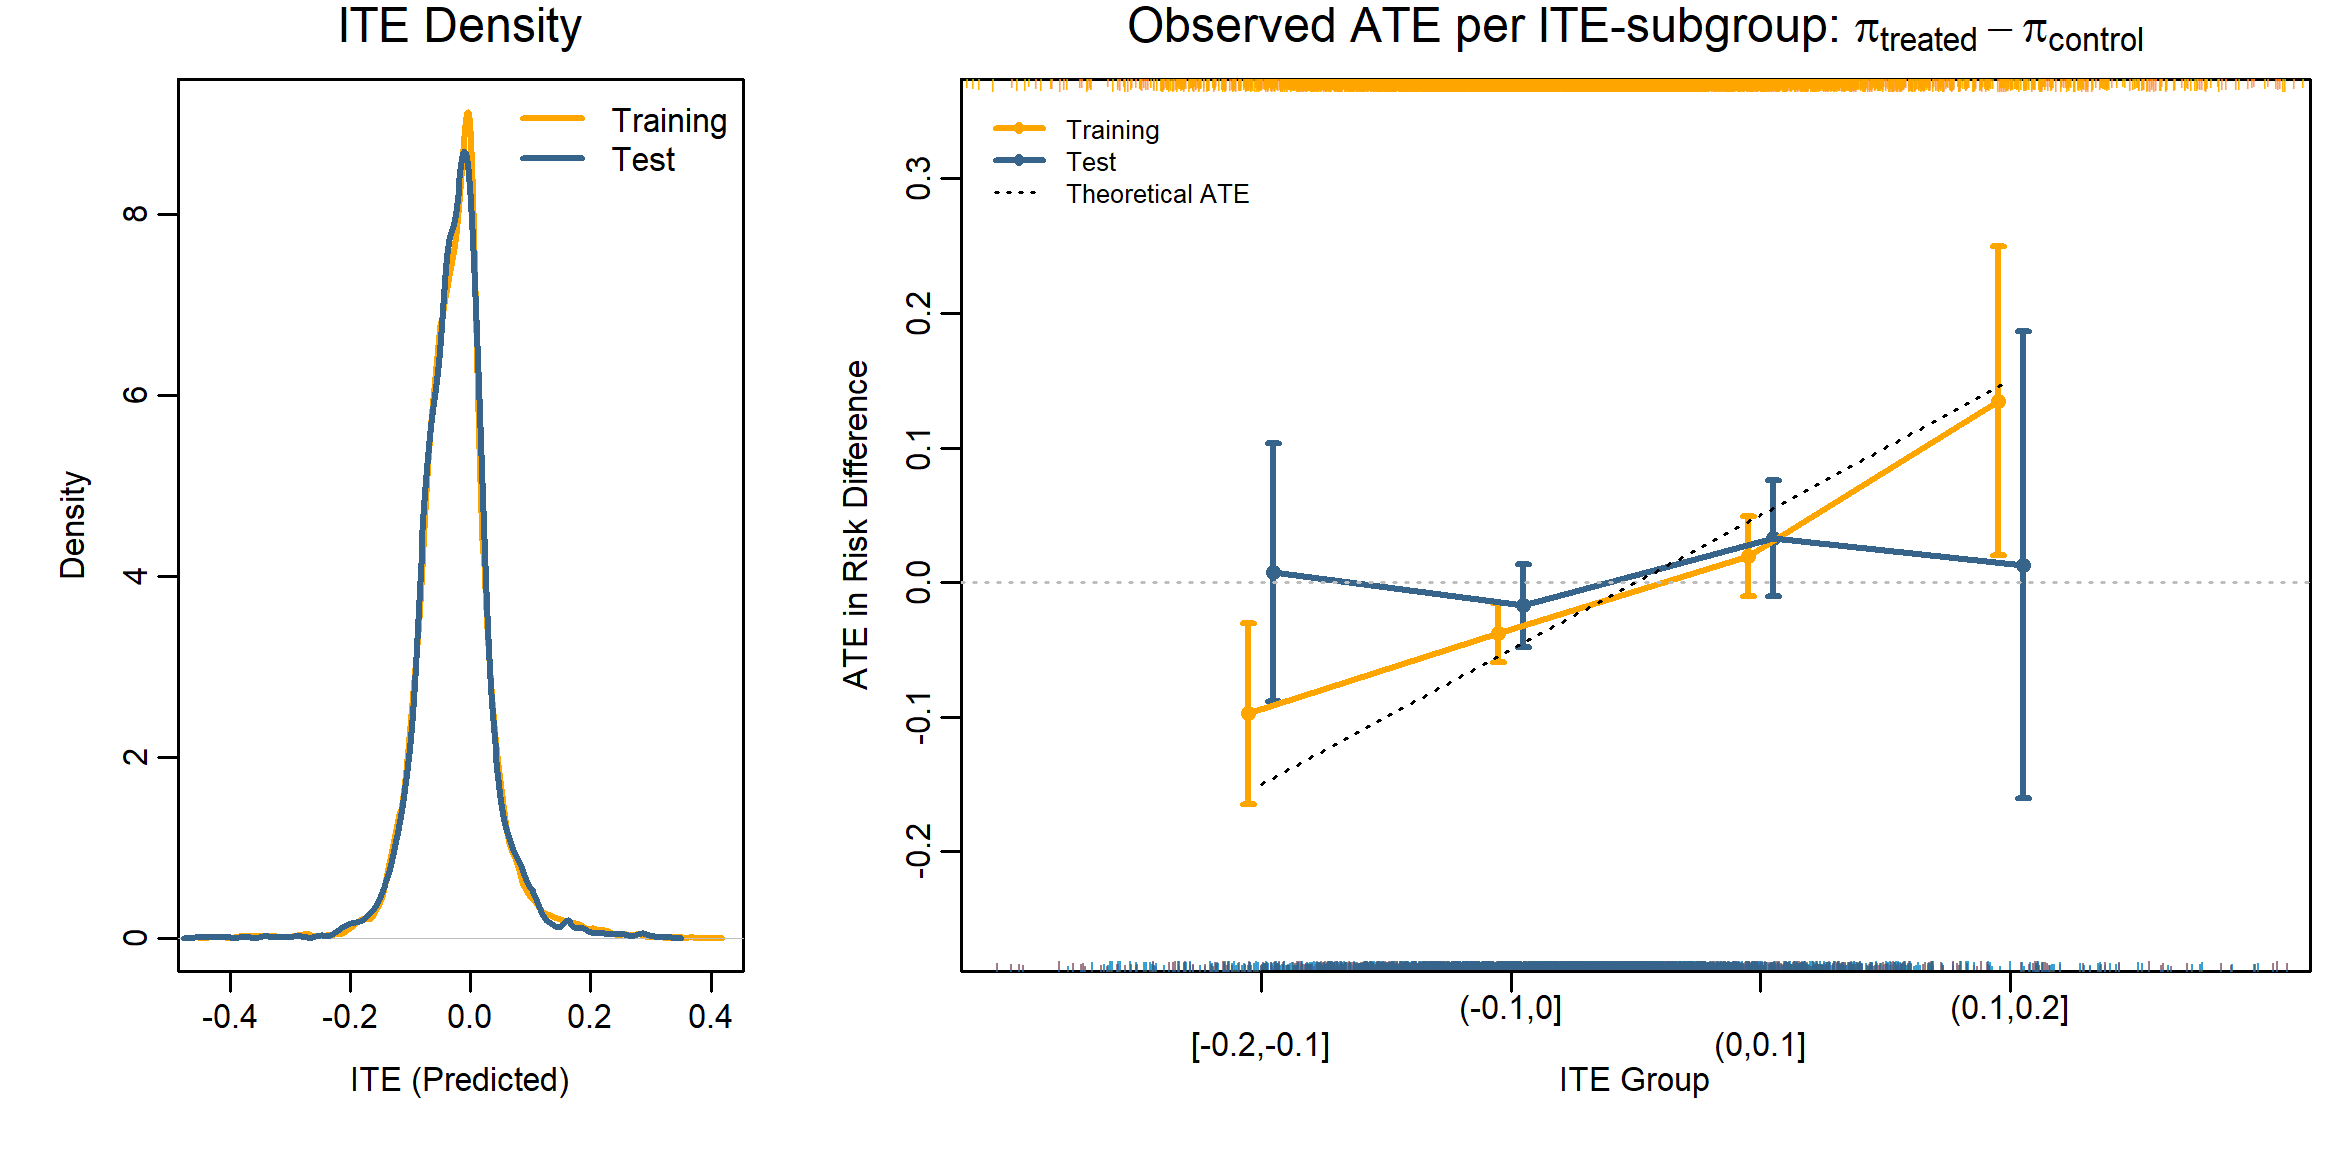
\includegraphics[width=\textwidth]{img/Experiment2/glm_tlearner_density_ITE_ATE.png}
% 
% \end{frame}
% 


\begin{frame}{Experiment 2: ITE on International Stroke Trial (IST): Results}

Results with T-learner tuned random forest (comets package):

% Below: image
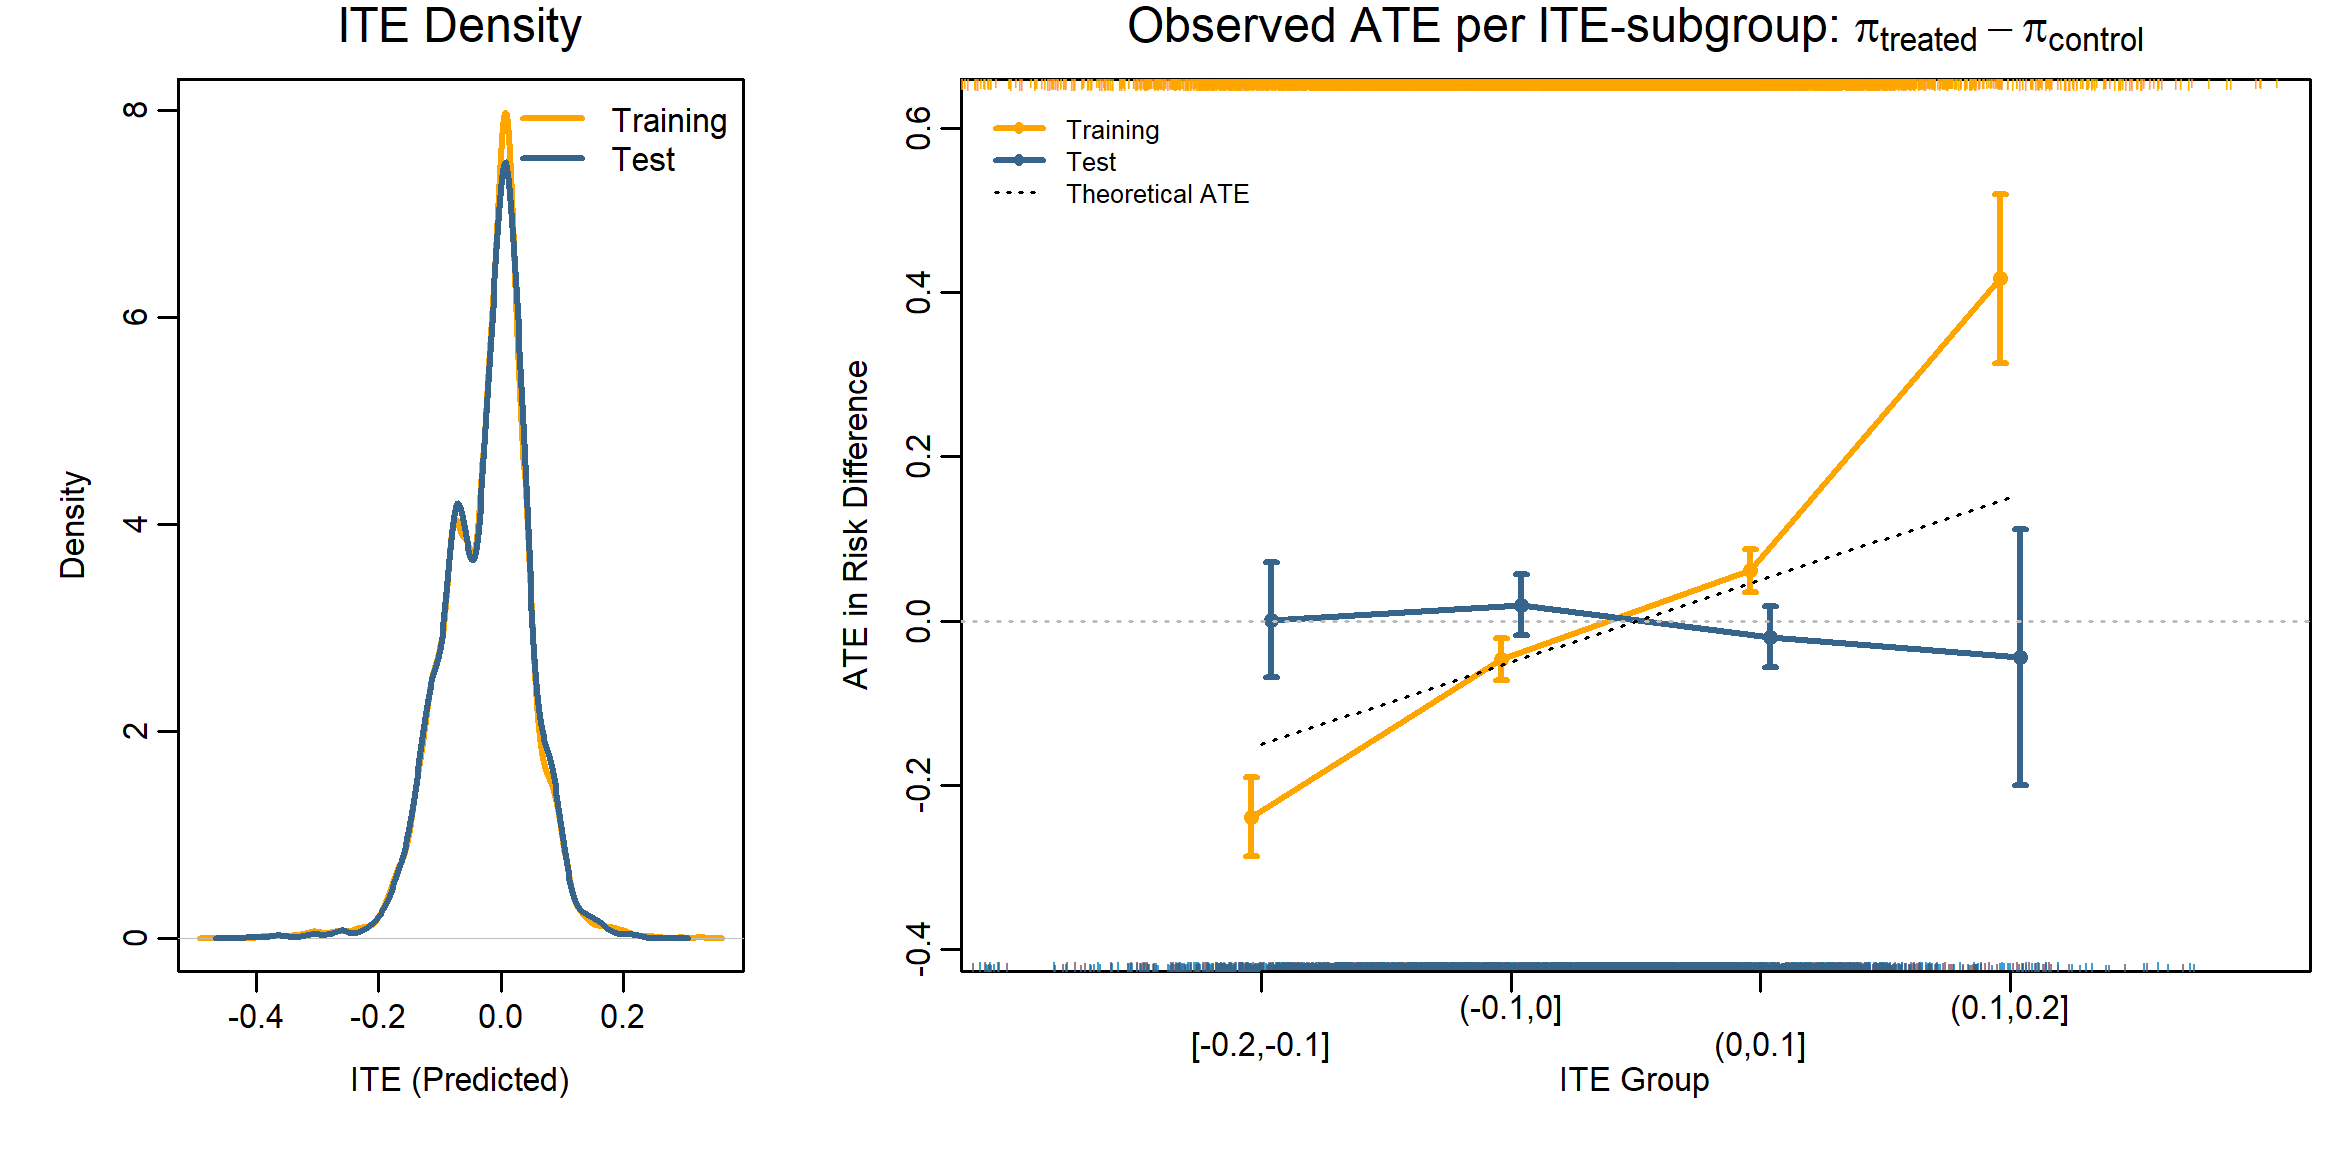
\includegraphics[width=\textwidth]{img/Experiment2/IST_tuned_rf_tlearner_density_ITE_ATE.png}

\end{frame}



\begin{frame}{Experiment 2: ITE on International Stroke Trial (IST): Discussion}

Our interpretation:

\begin{itemize}
    \item Similar results as \citet{chen2025}
    \item Some models suggest a range of ITEs, but do not generalize to the test set (no effect)
\end{itemize}

\end{frame}



% 
% \begin{frame}{Causal ML Models for ITE estimation}
% 
% Meta learners (T-learner, S-learner etc.)
% 
% 
% Tram dags
% 
% \end{frame}
% 
% 
% 
% 
% 
% \begin{frame}{IST Stroke trial}
% 
% 
% Explain the trial
% 
% \end{frame}
% 
% 
% 
% 
% 
% 
% \begin{frame}{IST Stroke trial: Results with GLM}
% 
% Show results of tlearner GLM
% 
% \end{frame}
% 
% 
% \begin{frame}{IST Stroke trial: Results with Random Forest}
% 
% 
% 
% 
% 
% 
% 
% 
% \end{frame}
% 
% 
% \begin{frame}{IST Stroke trial: Results with tram dag}
% 
% Show results of tram dag
% 
% \end{frame}
% 
% 
% 
% \begin{frame}{Simulation: When do problems occur?}
% 
% explain setup with dag and effect sizes and interactions that affect outcome
% 
% \end{frame}
% 
% 



\begin{frame}{Experiment 3: Simulation of ITE estimation robustness}

\textbf{Goal:}

\begin{itemize}
    \item Simulate different RCT scenarios to understand when ITE estimation fails
    \item Apply simple model (logistic regression) and complex model(tuned random forest)
\end{itemize}

\end{frame}




\begin{frame}{Simulation Case 1: Fully Observed}

\begin{columns}

% Left column: Text
\begin{column}{0.52\textwidth}

\vspace{-0.5em}
\textbf{Setup:}
\begin{itemize}\setlength\itemsep{0.4em}
  \item $n = 20{,}000$
  \item $T \sim \text{Bernoulli}(0.5)$
  \item $\mathbf{X} = (X_1, \dots, X_5)^\top \sim \mathcal{N}(\mathbf{0}, \Sigma)$\\
  \item $\mathbf{X_{TX}} = (X_1, X_2)^\top$ \textcolor{red}{interaction}
\end{itemize}


\end{column}

% Right column: DAG image
\begin{column}{0.42\textwidth}
    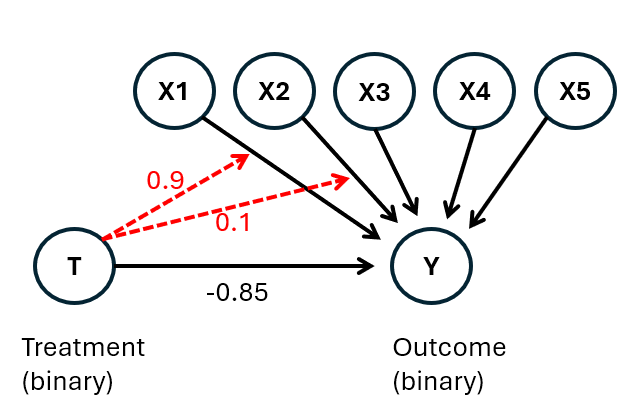
\includegraphics[width=\textwidth]{img/simulation_observed.png}
\end{column}

\end{columns}


\vspace{0.3em}
\textbf{Outcome model:}
\[
\mathbb{P}(Y = 1 \mid \mathbf{X}, T) = \text{logit}^{-1} \left(
\beta_0 + \beta_T T + \boldsymbol{\beta}_X^\top \mathbf{X}
+ \textcolor{red}{T \cdot \boldsymbol{\beta}_{TX}^\top \mathbf{X_{TX}}}
\right)
\]


\end{frame}





\begin{frame}{Simulation Case 1: Fully Observed}

Results with T-learner logistic regression (glm):

% Below: image
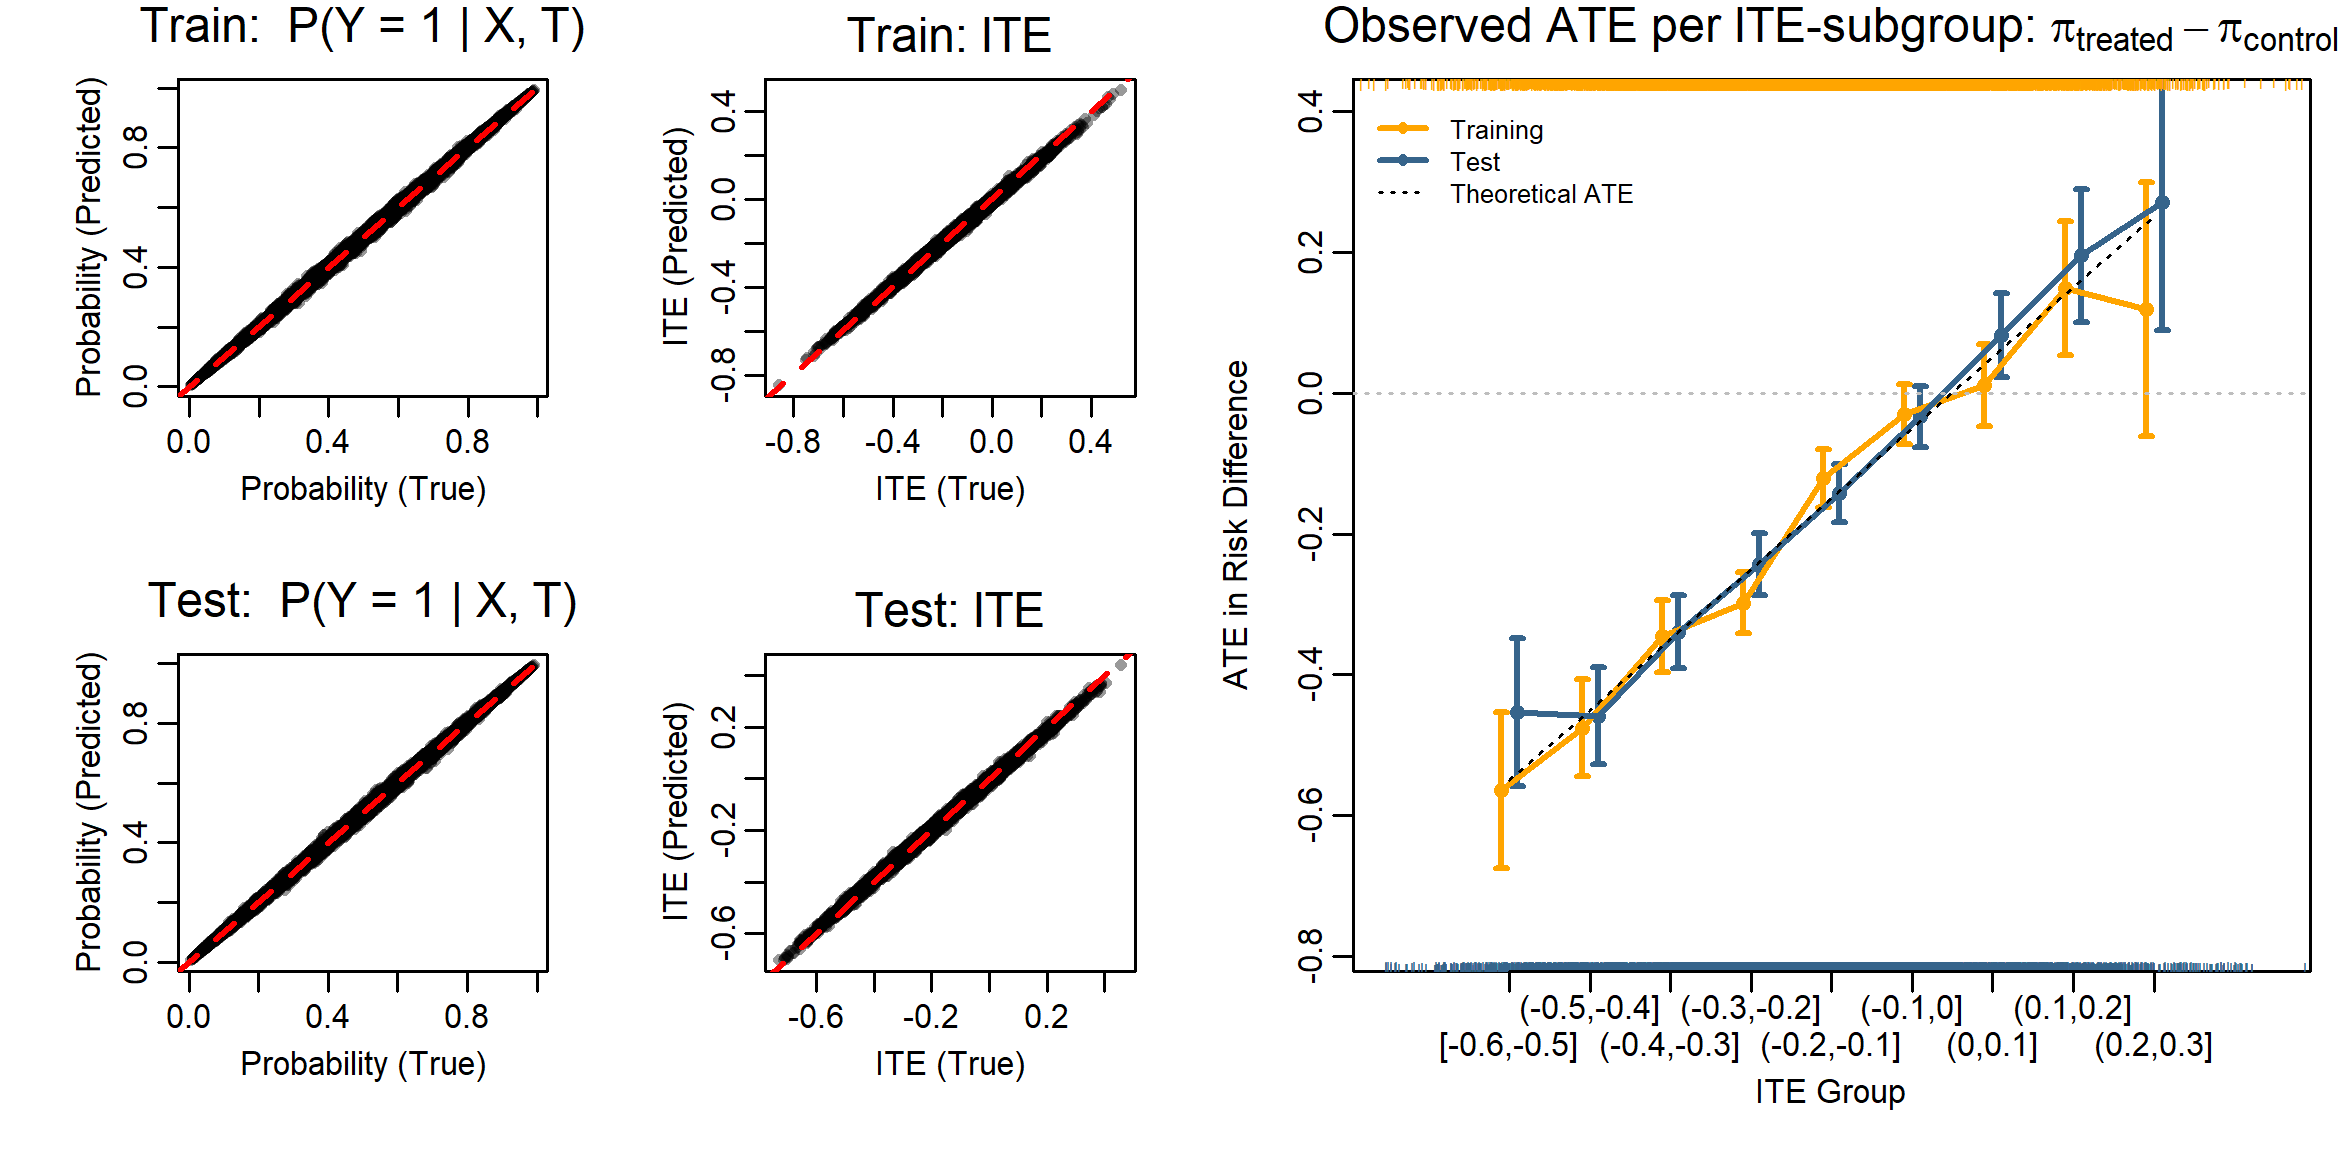
\includegraphics[width=\textwidth]{img/fully_observed_glm_tlearner.png}

\end{frame}


\begin{frame}{Simulation Case 1: Fully Observed}

Results with T-learner Random Forest (comets package):

% Below: image
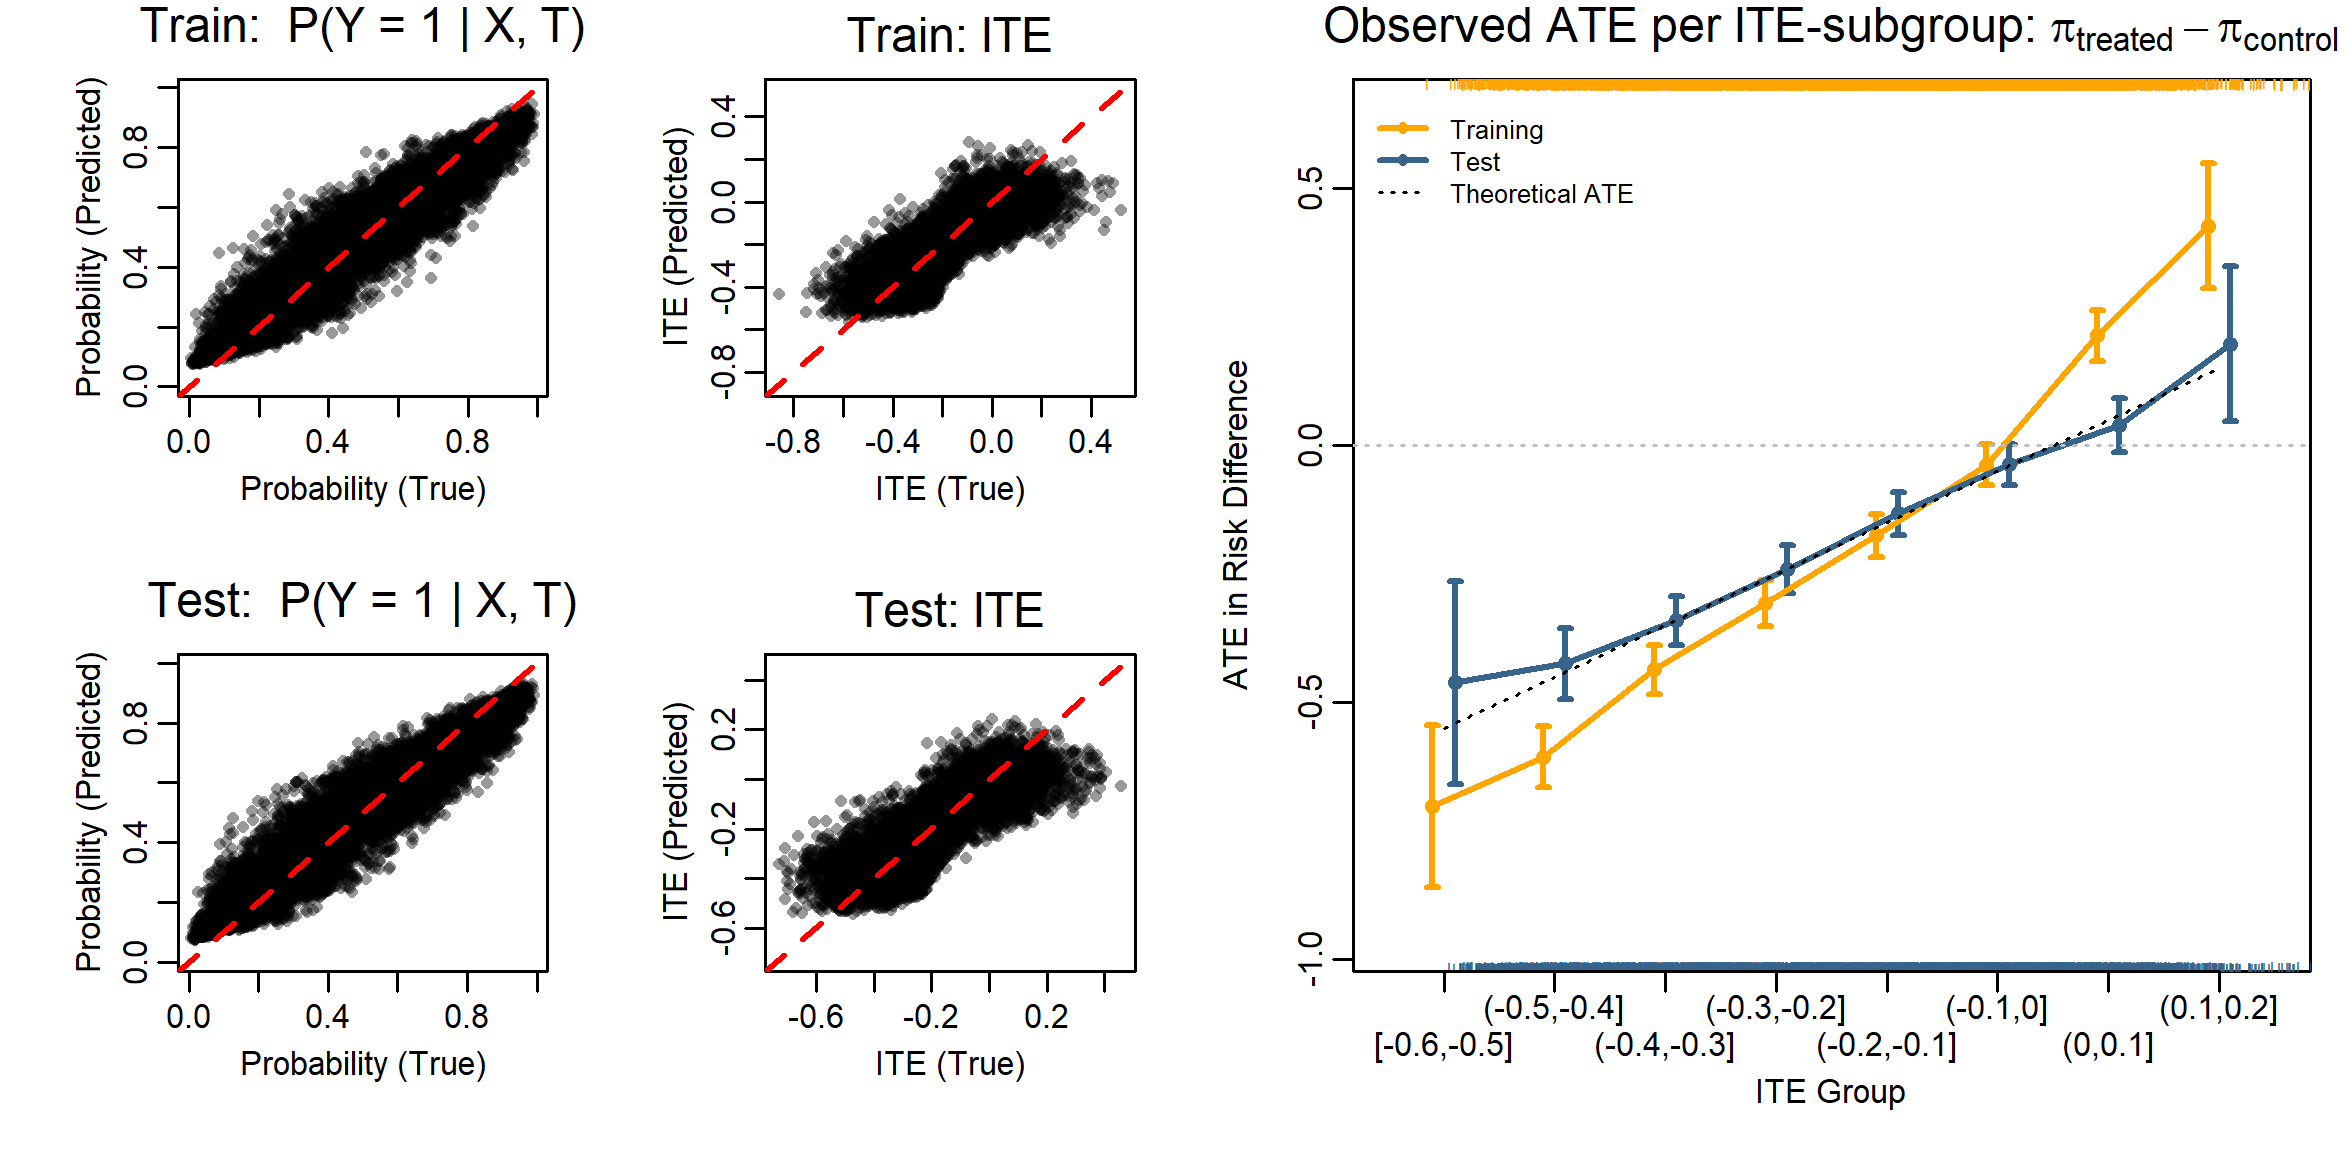
\includegraphics[width=\textwidth]{img/observed_tuned_rf.png}

\end{frame}







\begin{frame}{Simulation Case 2: Unobserved Interaction}

\begin{columns}

% Left column: Text
\begin{column}{0.52\textwidth}

\vspace{-0.5em}
\textbf{Setup:}
\begin{itemize}\setlength\itemsep{0.4em}
  \item $n = 20{,}000$
  \item $T \sim \text{Bernoulli}(0.5)$
  \item $\mathbf{X} = (X_1, \dots, X_5)^\top \sim \mathcal{N}(\mathbf{0}, \Sigma)$\\
  \item $\mathbf{X_{TX}} = (X_1, X_2)^\top$ \textcolor{red}{interaction}
\end{itemize}


\end{column}

% Right column: DAG image
\begin{column}{0.42\textwidth}
    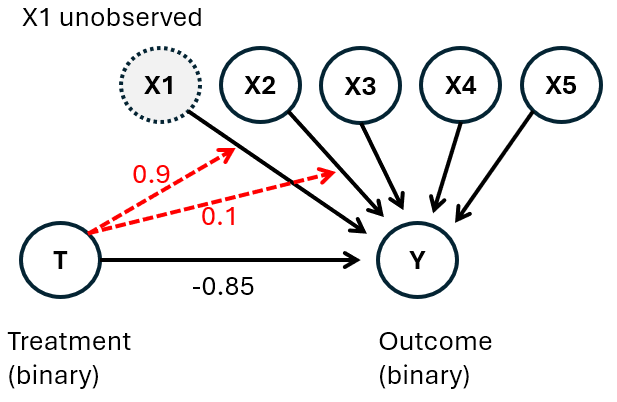
\includegraphics[width=\textwidth]{img/simulation_unobserved.png}
\end{column}

\end{columns}


\vspace{0.3em}
\textbf{Outcome model:}
\[
\mathbb{P}(Y = 1 \mid \mathbf{X}, T) = \text{logit}^{-1} \left(
\beta_0 + \beta_T T + \boldsymbol{\beta}_X^\top \mathbf{X}
+ \textcolor{red}{T \cdot \boldsymbol{\beta}_{TX}^\top \mathbf{X_{TX}}}
\right)
\]

% in this scenario X1 is unobserved
\textbf{Note:} Same DGP, but $X_1$ is not observed!

\end{frame}




\begin{frame}{Simulation Case 2: Unobserved Interaction}

Results with T-learner logistic regression (glm):

% Below: image
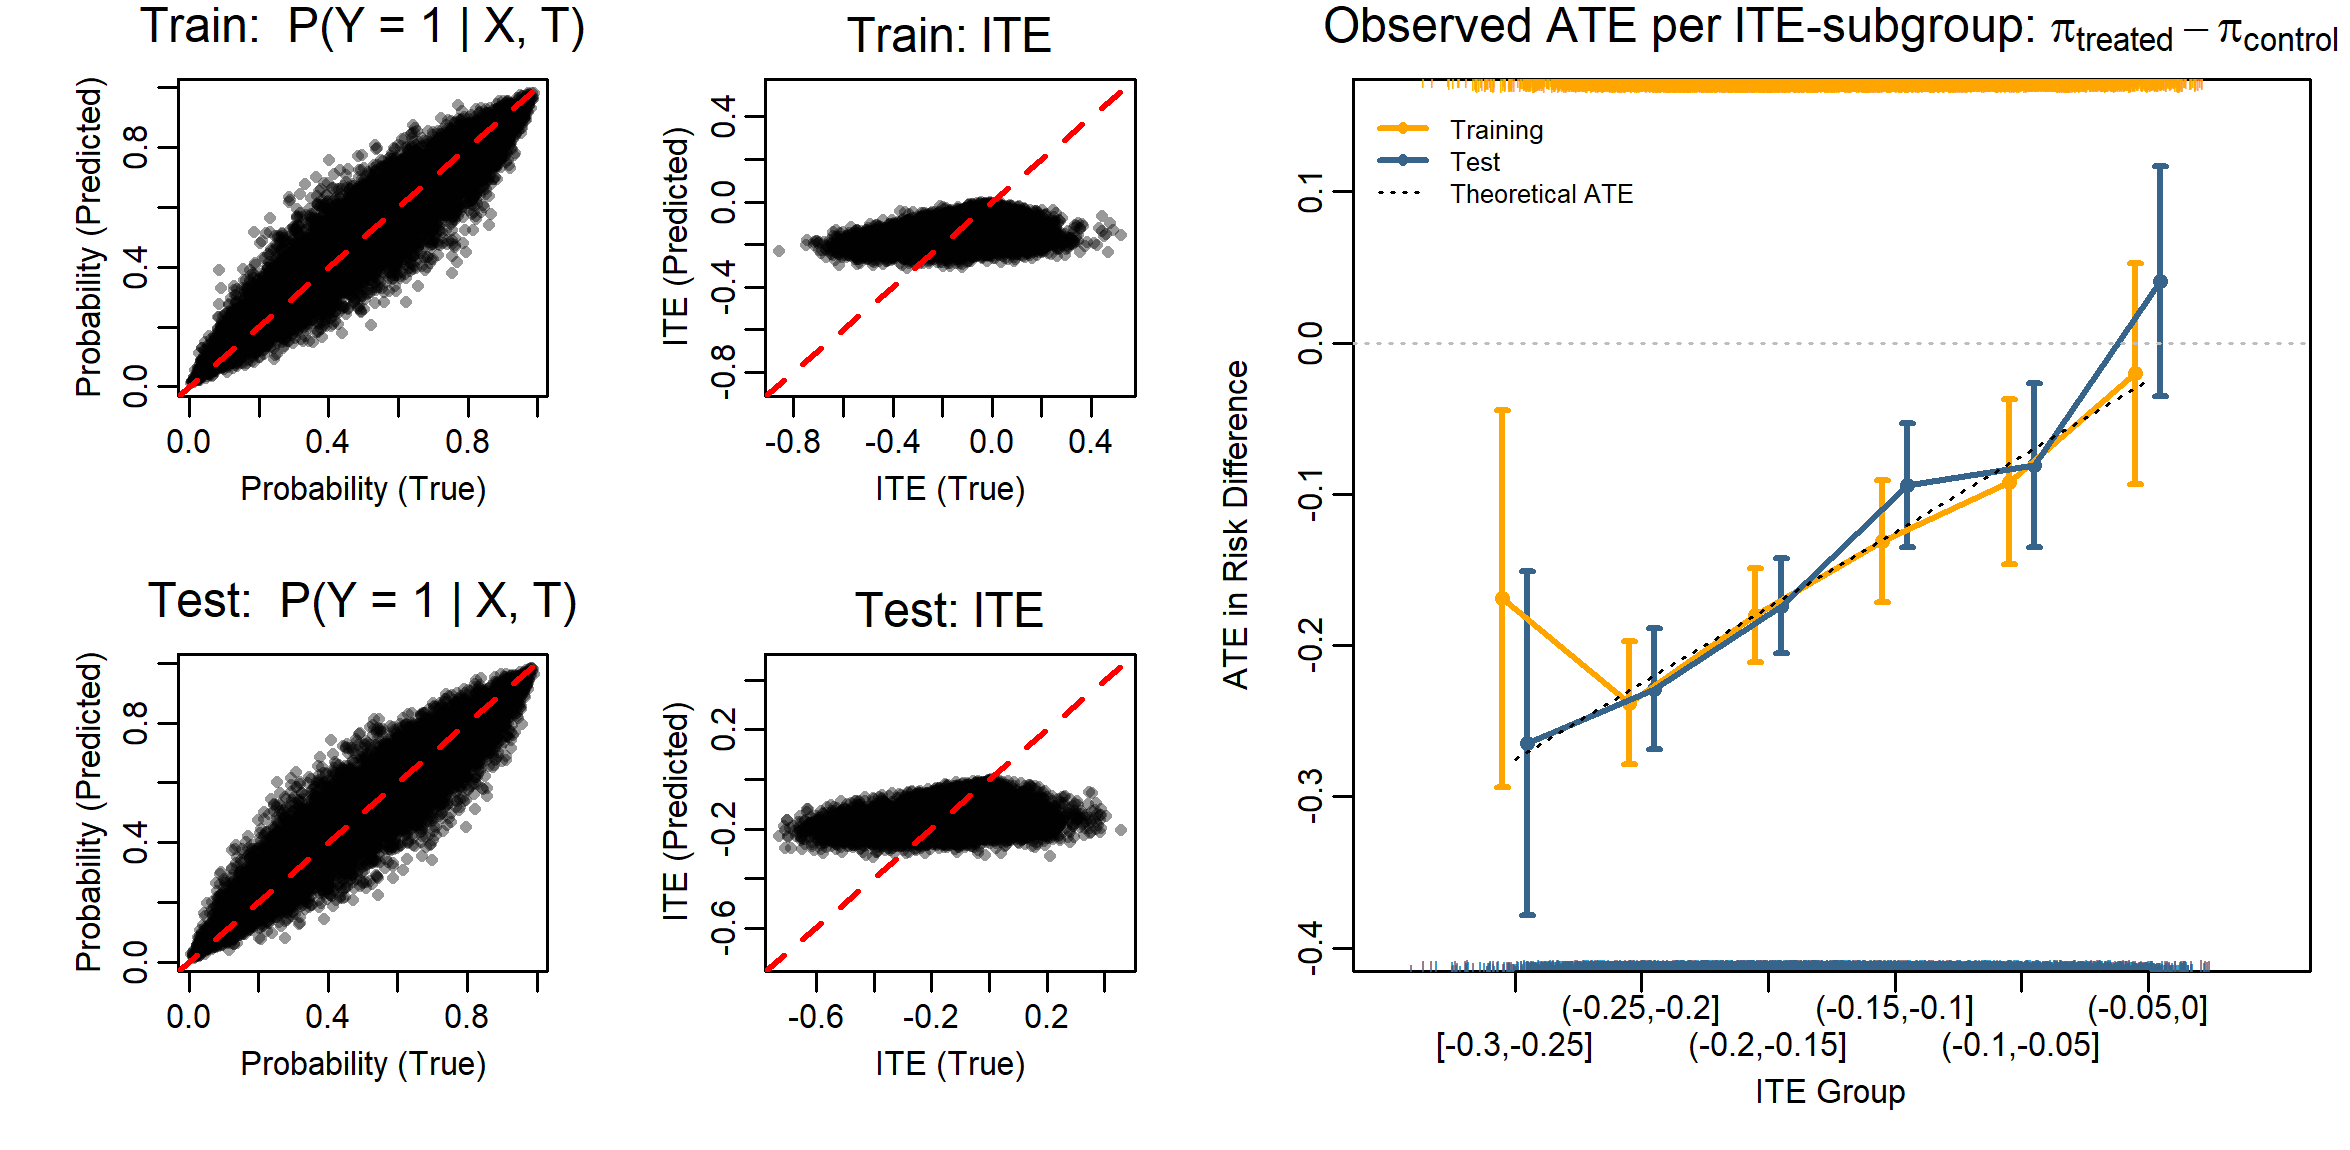
\includegraphics[width=\textwidth]{img/unobserved_interaction_glm_tlearner.png}

\end{frame}

\begin{frame}{Simulation Case 2: Unobserved Interaction}

Results with T-learner Random Forest (comets):

% Below: image
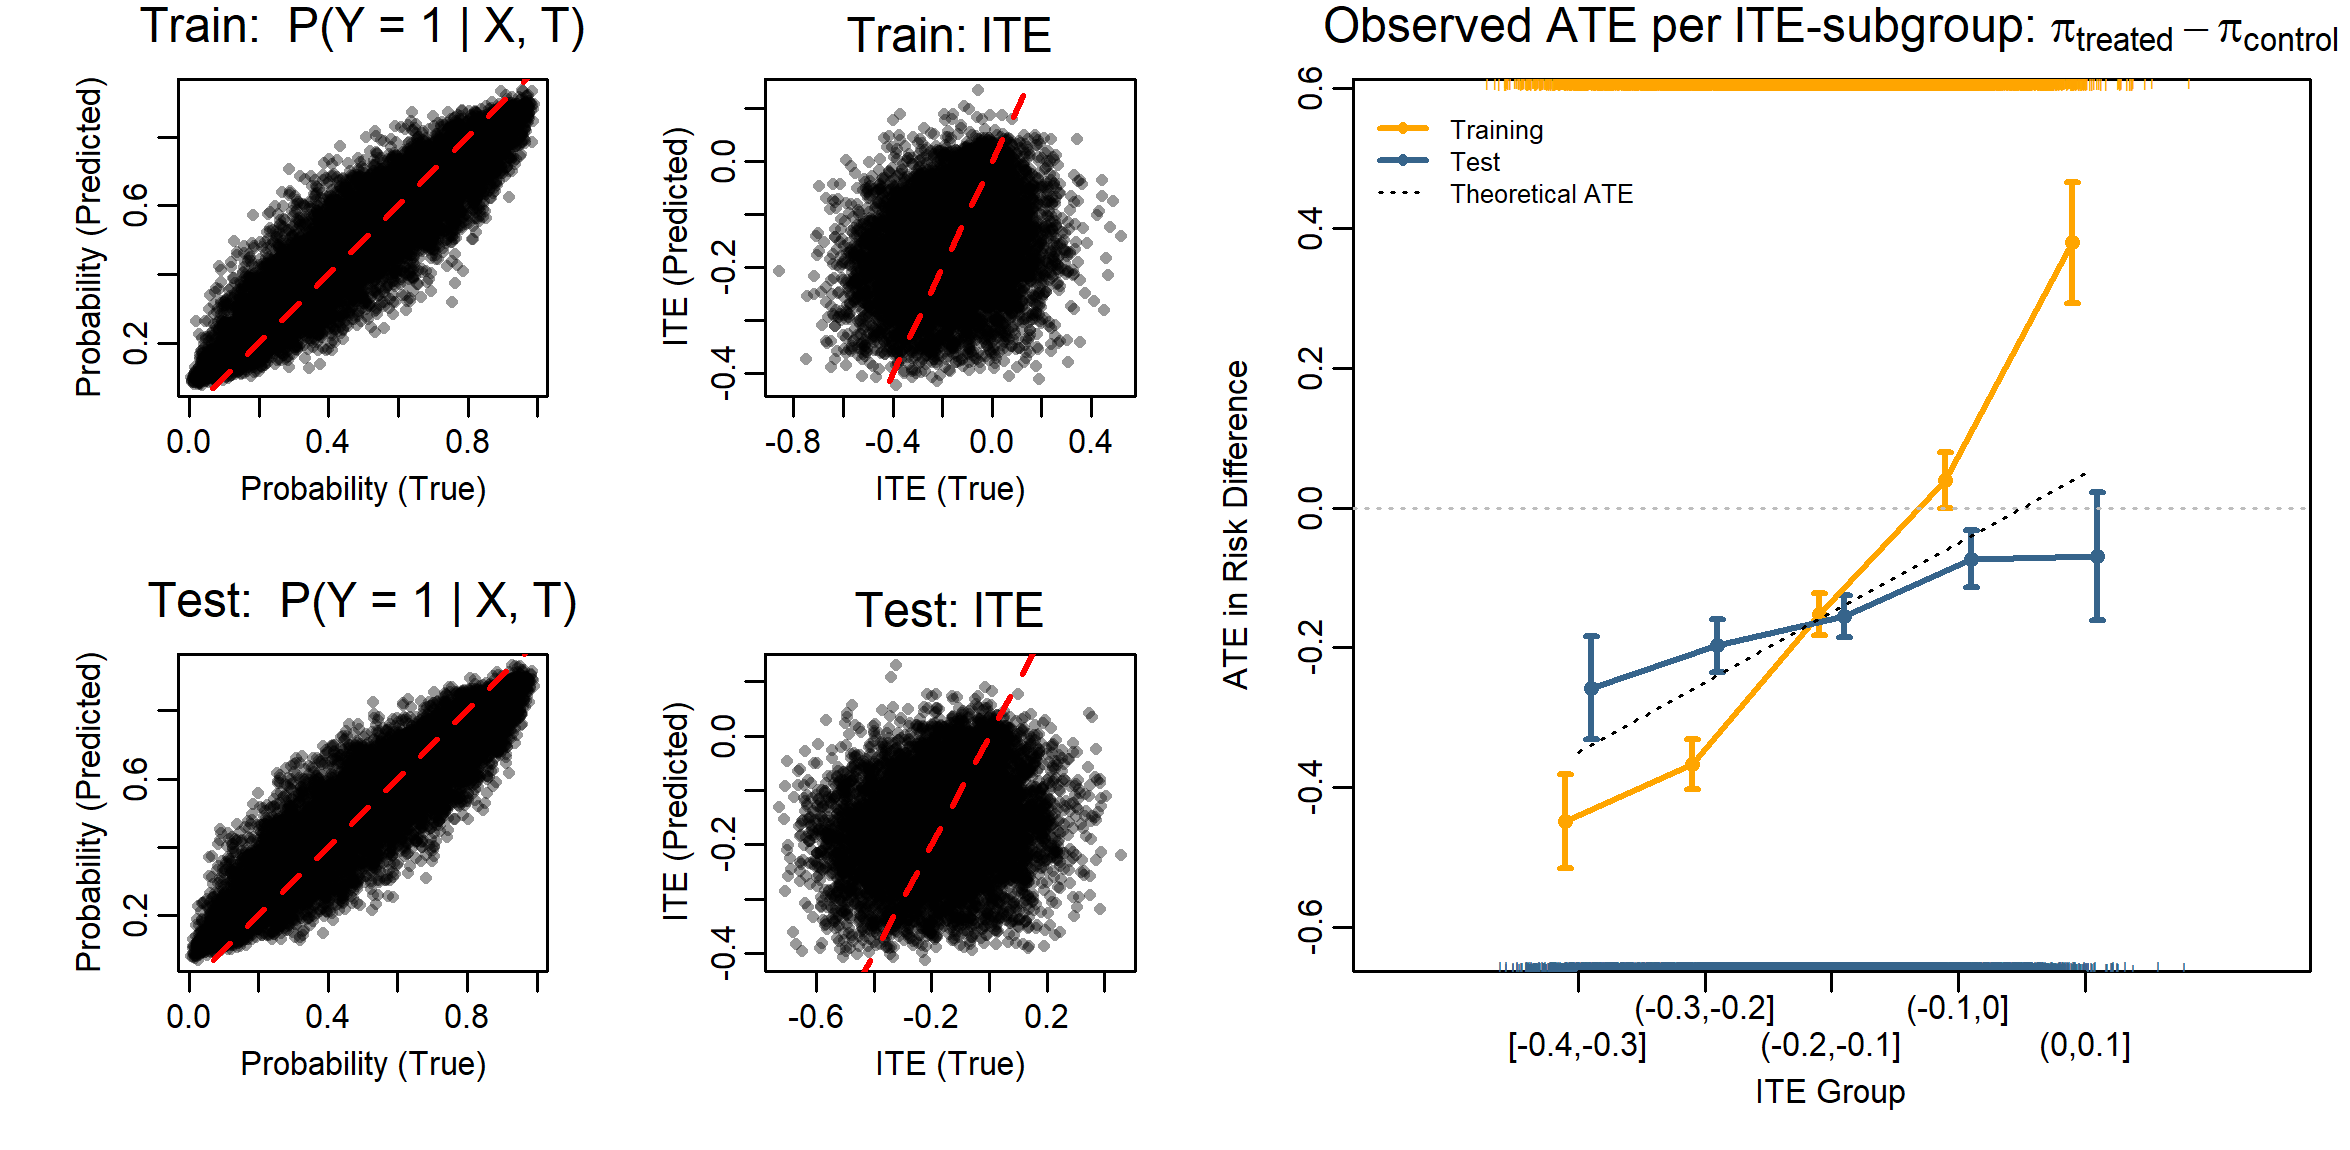
\includegraphics[width=\textwidth]{img/unobserved_tuned_rf.png}

\end{frame}





\begin{frame}{Simulation Case 3: Fully Observed, Small Effects}

\begin{columns}

% Left column: Text
\begin{column}{0.52\textwidth}

\vspace{-0.5em}
\textbf{Setup:}
\begin{itemize}\setlength\itemsep{0.4em}
  \item $n = 20{,}000$
  \item $T \sim \text{Bernoulli}(0.5)$
  \item $\mathbf{X} = (X_1, \dots, X_5)^\top \sim \mathcal{N}(\mathbf{0}, \Sigma)$\\
  \item $\mathbf{X_{TX}} = (X_1, X_2)^\top$ \textcolor{red}{interaction}
\end{itemize}


\end{column}

% Right column: DAG image
\begin{column}{0.42\textwidth}
    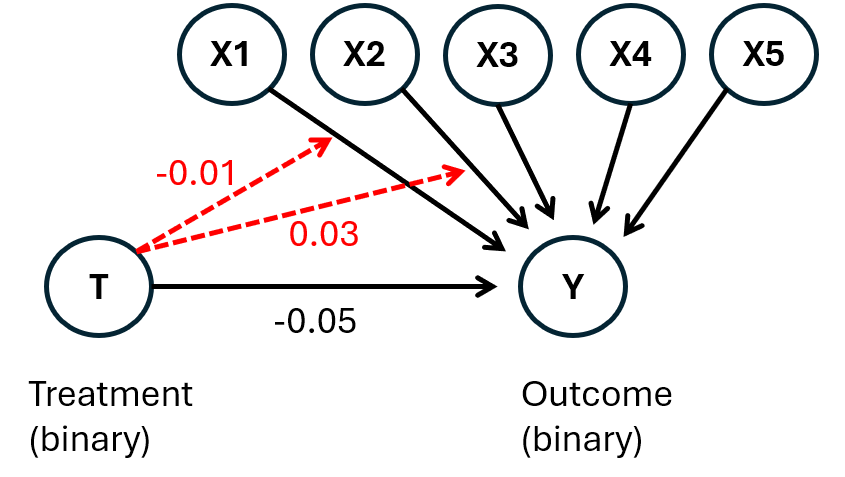
\includegraphics[width=\textwidth]{img/simulation_small_effects.png}
\end{column}

\end{columns}


\vspace{0.3em}
\textbf{Outcome model:}
\[
\mathbb{P}(Y = 1 \mid \mathbf{X}, T) = \text{logit}^{-1} \left(
\beta_0 + \beta_T T + \boldsymbol{\beta}_X^\top \mathbf{X}
+ \textcolor{red}{T \cdot \boldsymbol{\beta}_{TX}^\top \mathbf{X_{TX}}}
\right)
\]

\textbf{Note:} Same DGP, but weak treatment effects!


\end{frame}





\begin{frame}{Simulation Case 3: Fully Observed, Small Effects}

Results with T-learner logistic regression (glm):

% Below: image
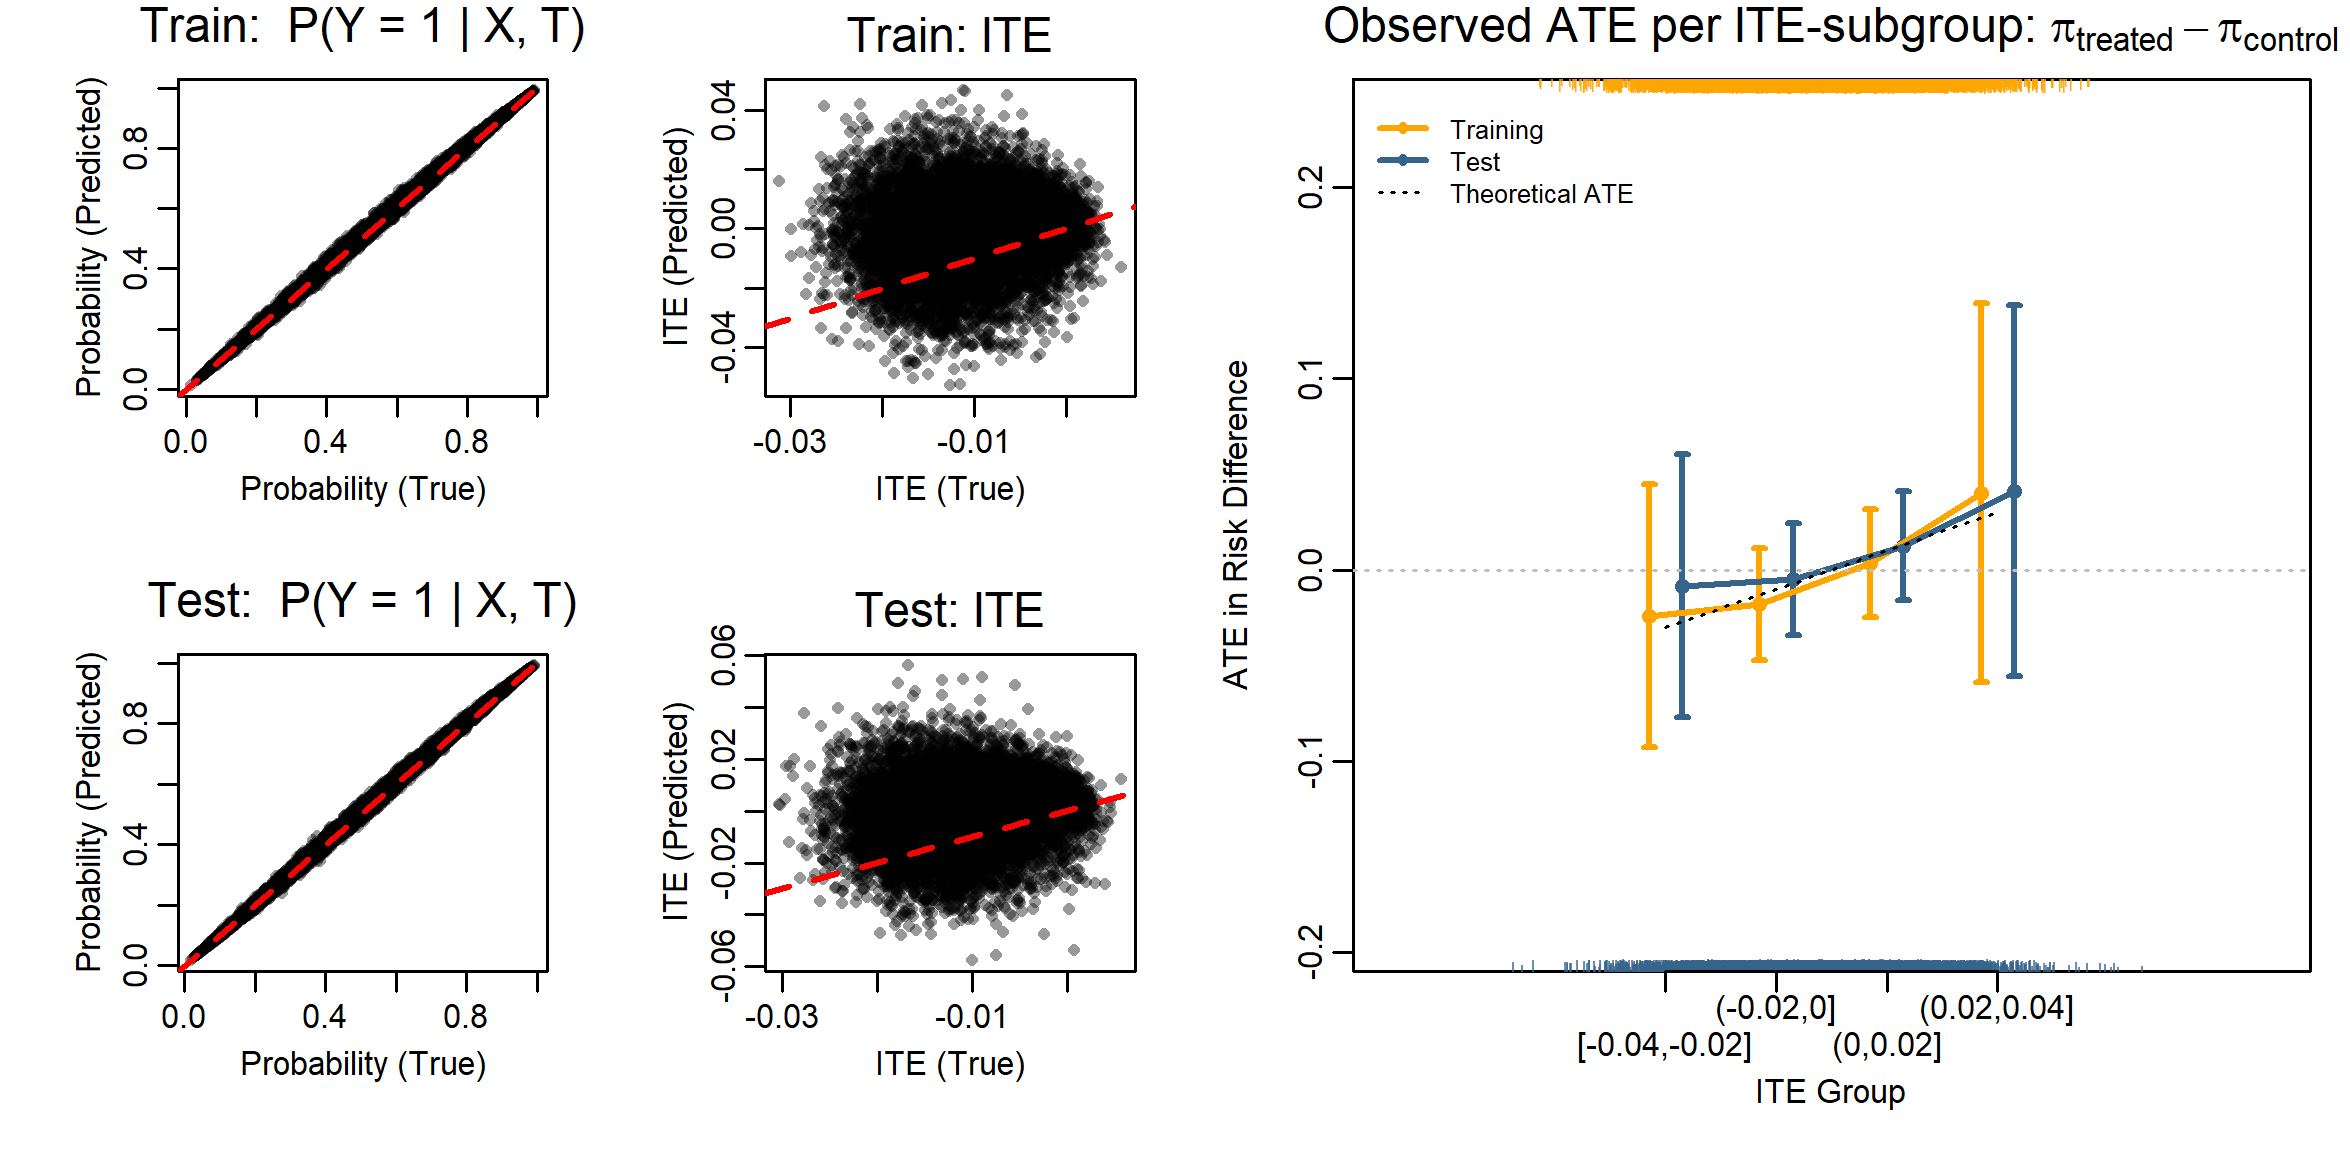
\includegraphics[width=\textwidth]{img/small_interaction_glm_tlearner.png}

\end{frame}


\begin{frame}{Simulation Case 3: Fully Observed, Small Effects}

Results with T-learner Random Forest (comets package):

% Below: image
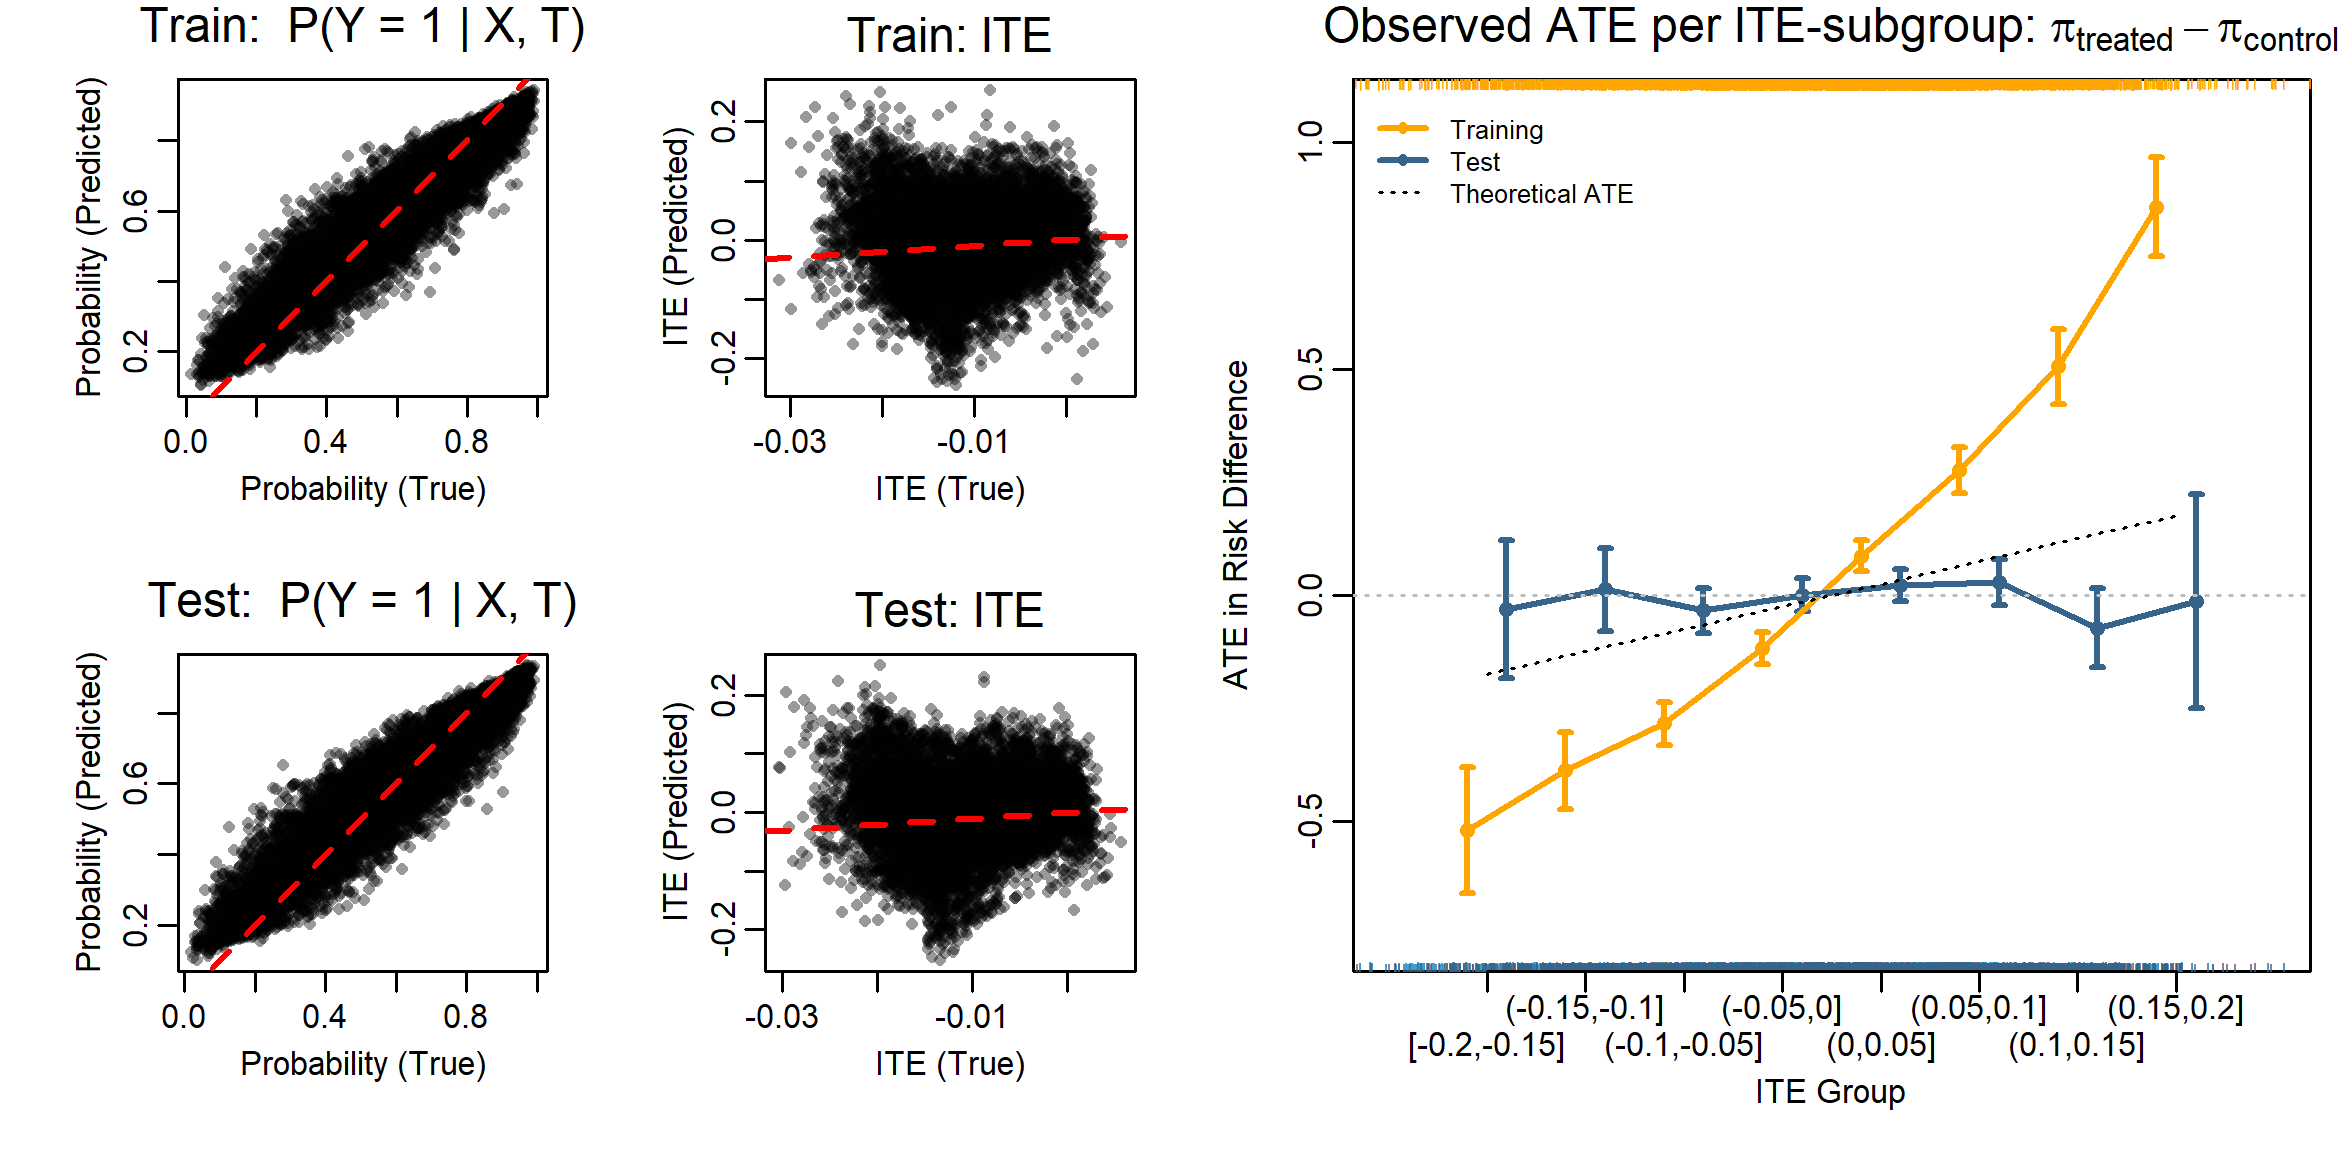
\includegraphics[width=\textwidth]{img/small_interaction_tuned_rf_tlearner.png}

\end{frame}





\begin{frame}{ITE simulation: Interpretation}

\textbf{My interpretation:} 
\begin{itemize}
    \item When a high predicted treatment effect (ITE) corresponds to a high observed effect in the train set (strong discrimination), but not in the test set, it might be due to \textbf{unobserved interaction variables} or \textbf{weak treatment effects}.
    \item This is more likely to occur with complex models, as they tend to overfit when the interaction is not observed.
    % as they tend to predict a wider range of ITEs than simpler models
\end{itemize}


\end{frame}




% 
% \begin{frame}{TRAM-DAGs for ITE Estimation}
% 
% \begin{columns}
% 
% % Left side: Text (approx. 3/4 of the slide)
% \begin{column}{0.7\textwidth}
% 
% \textbf{Paper \textit{"Interpretable Neural Causal Models with TRAM-DAGs"} \citep{sick2025}:}
% \begin{itemize}
%     \item Framework to model causal relationships
%     \item Based on transformation models
%     \item Rely on (deep) neural networks
%     \item Compromise between interpretability and flexibility
% \end{itemize}
% 
% \textbf{Our Claim:} We can use TRAM-DAGs for ITE estimation, as long as the DAG is known and fully observed!
% 
% \end{column}
% 
% % Right side: Image (approx. 1/4 of the slide)
% \begin{column}{0.3\textwidth}
% 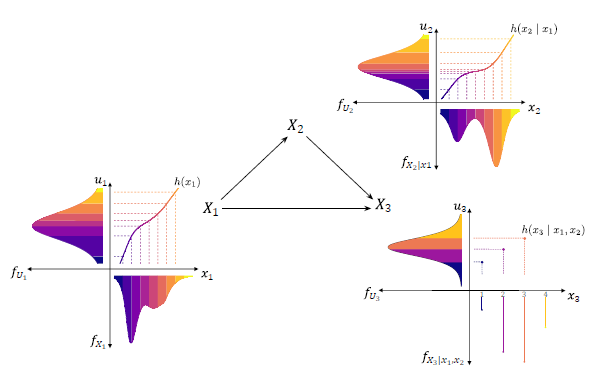
\includegraphics[width=\textwidth]{img/TRAM_DAG_Background.png}
% \end{column}
% 
% \end{columns}
% 
% \end{frame}
% 
% 


% 
% \begin{frame}{TRAM-DAGs: Structural Equations}
% 
% 
% TRAM-DAGs estimate the structural equations with transformation functions $h_i$:
% 
% \begin{columns}
% 
% % Left side: Text
% \begin{column}{0.5\textwidth}
% 
% $Z_i = h_i(X_i \mid \text{pa}(X_i))$ \\
% $X_i = h_i^{-1}(Z_i, \text{pa}(X_i)) = f_i(Z_i, \text{pa}(X_i))$ \\
% 
% %empty line
% \vspace{1.5em}
% 
% \begin{itemize}
%     \item $\text{pa}(X_i)$: causal parents of $X_i$
%     \item $Z_i$: noise distribution (e.g. standard logistic)
% \end{itemize}
% 
% \end{column}
% 
% % Right side: Image
% \begin{column}{0.5\textwidth}
% 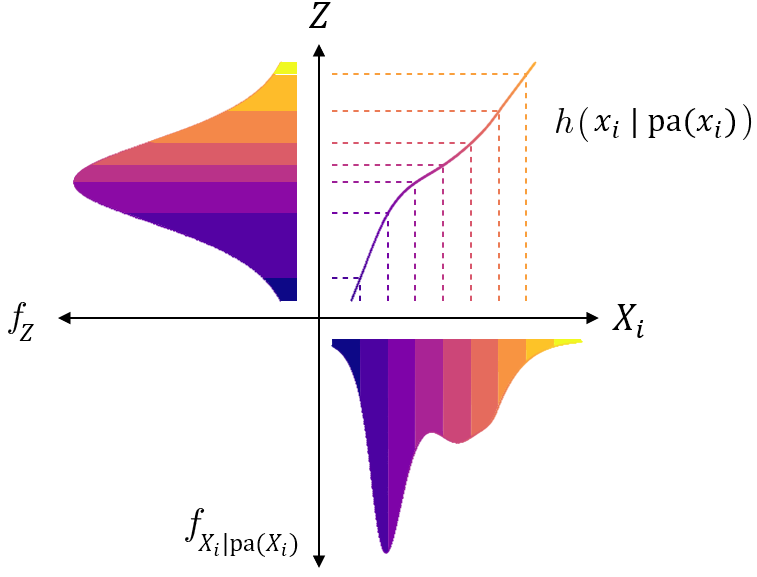
\includegraphics[width=\textwidth]{img/trafo_xi.png}
% \end{column}
% \end{columns}
% 
% 
% \end{frame}





\begin{frame}{TRAM-DAGs: Example for ITE estimation}

\centering
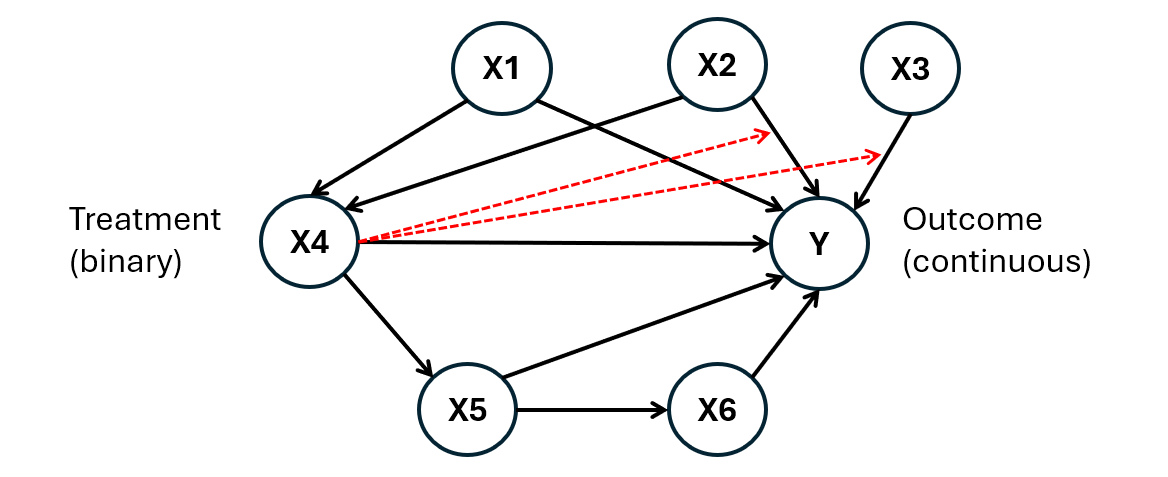
\includegraphics[width=0.8\textwidth]{img/dag_ITE_observational.png}
\normalsize

\vspace{1em} % optional spacing
\raggedright % <--- Ends centering and left-aligns following text

\small
\textbf{DGP:}
\begin{itemize}
    \item $X5 = h_5^{-1}(\epsilon - 0.8 \, X4 )$ \hspace{1em} $\rightarrow$ (depends on treatment)
    \item $X6 = h_6^{-1}(\epsilon + 0.5 \, X5)$ \hspace{1em} $\rightarrow$ (depends on treatment through X5)
    \item $Y = h_7^{-1}(\epsilon - \beta_1 X1 - \beta_2 X2 - \beta_3 X3 - \beta_4 X4 - \beta_5 X5 - \beta_6 X6 - \textcolor{red}{Tr \cdot (\beta_{2Tr} X2 + \beta_{3Tr} X3)})$
\end{itemize}

\end{frame}






\begin{frame}{TRAM-DAGs: Estimate Potential Outcomes}

If we observe a $X5$ under $Tr=0$, we can determine the counterfactual $X5$ under $Tr=1$ with the observed latent value $z_j$:

\centering
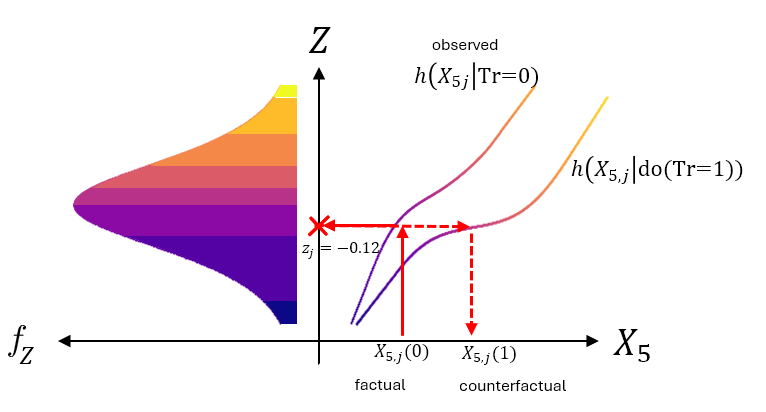
\includegraphics[width=0.7\textwidth]{img/counterfactual_X5.png}

\end{frame}





\begin{frame}{TRAM-DAGs: Example for ITE estimation}

\[
\text{ITE} = \operatorname{median}(Y \mid \text{do}(T = 1), X) - \operatorname{median}(Y \mid \text{do}(T = 0), X)
\]

\centering

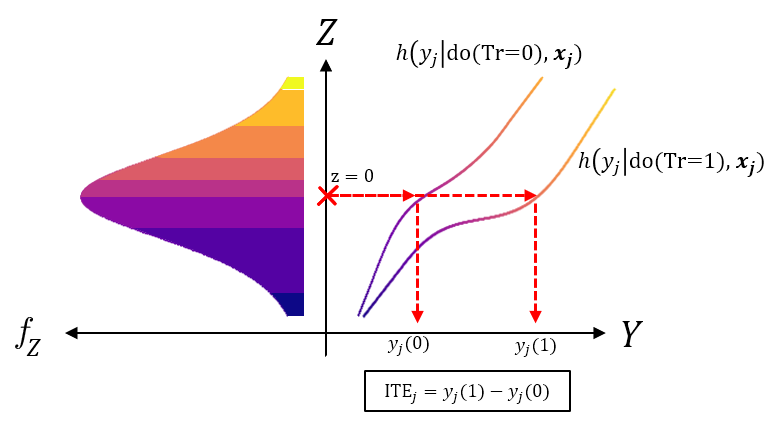
\includegraphics[width=0.7\textwidth]{img/potential_outcomes_y.png}



\end{frame}





\begin{frame}{TRAM-DAGs: Example for ITE estimation}

\[
\text{ITE} = \operatorname{median}(Y \mid \text{do}(T = 1), X) - \operatorname{median}(Y \mid \text{do}(T = 0), X)
\]

\centering
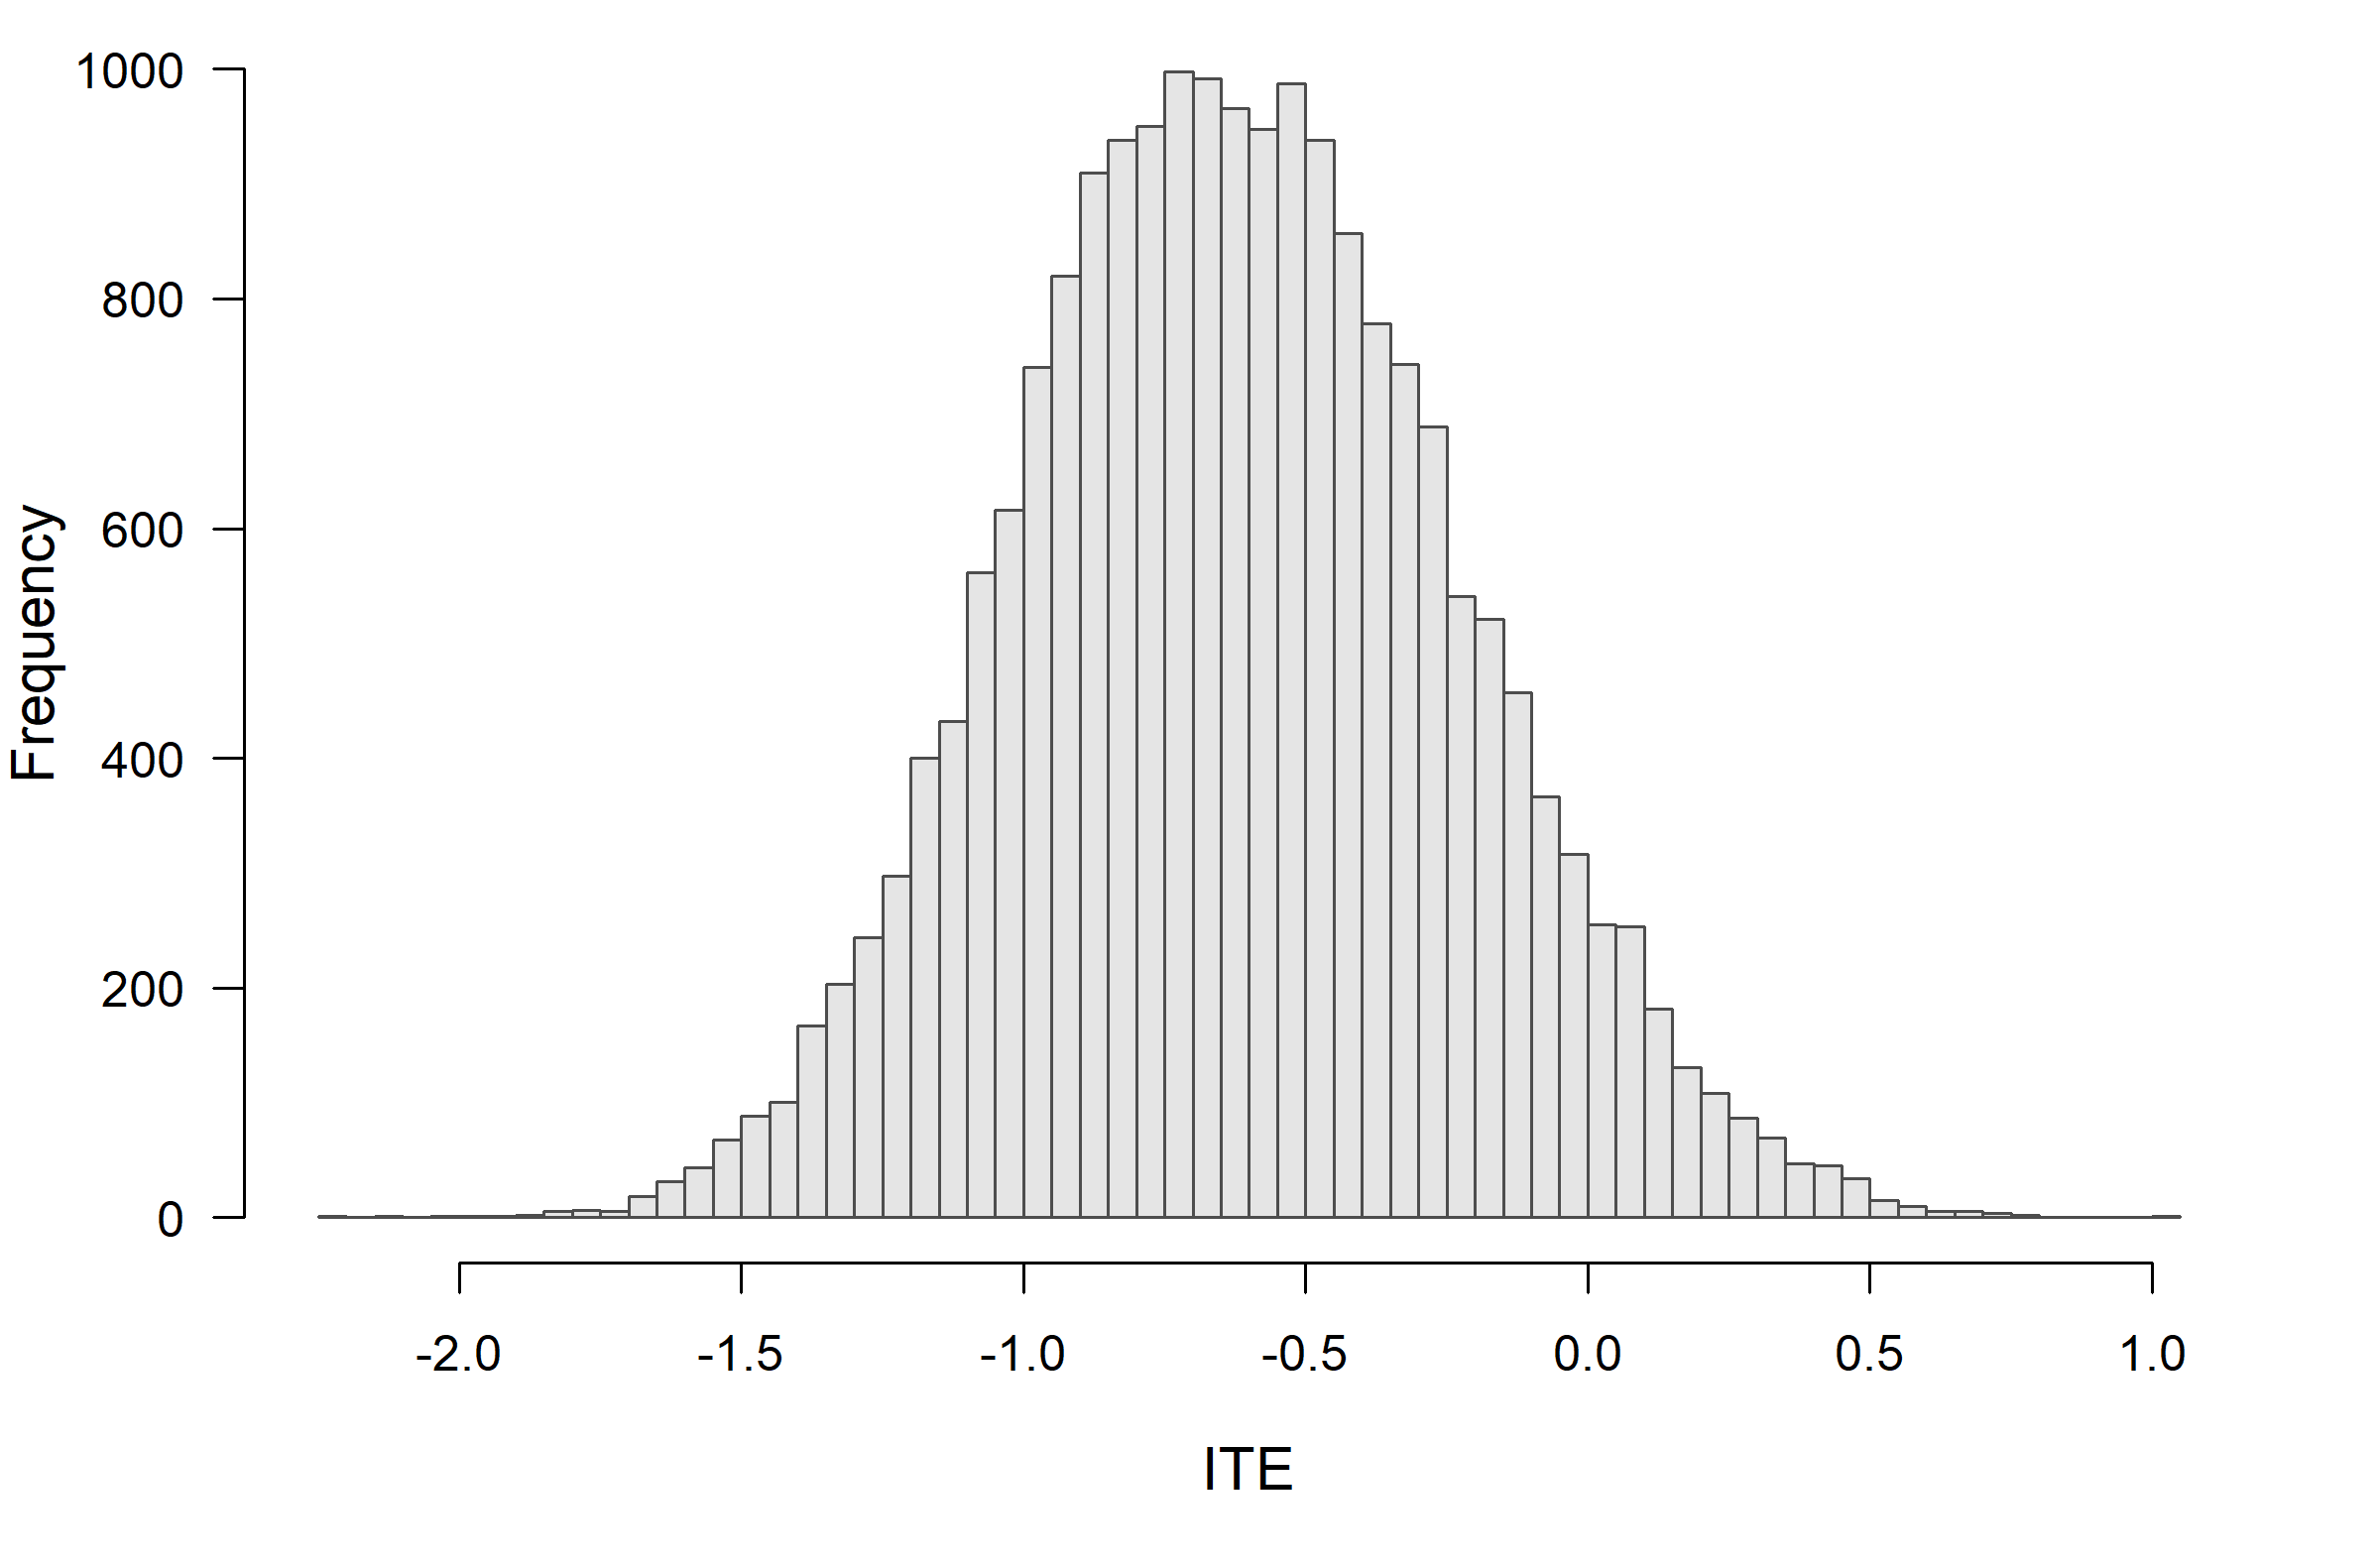
\includegraphics[width=0.7\textwidth]{img/observ_scenario1_ite_distribution_dgp.png}

\end{frame}




\begin{frame}{TRAM-DAGs: Estimate Potential Outcomes}


\begin{enumerate}
    \item Estimate each $h_i(X_i \mid \text{pa}(X_i))$ fully flexible (deep-NN / complex intercept)
    \item Take the train set or a test set
    \item $Z_i = h(X_i \mid pa(X_i))$ gives us the (observed) latent variable for each $X_i$
    \item Determine counterfactuals for X5 and X6 with the (observed) latent variables $Z_i$
    \item Determine medians of potential outcomes $Y(1)$ and $Y(0)$
    \item $\text{ITE} = \text{median}(Y(1) \mid X_{tx}) - \text{median}(Y(0) \mid X_{ct})$
\end{enumerate}

\end{frame}






\begin{frame}{TRAM-DAGs: Example for ITE estimation (Results)}


\centering
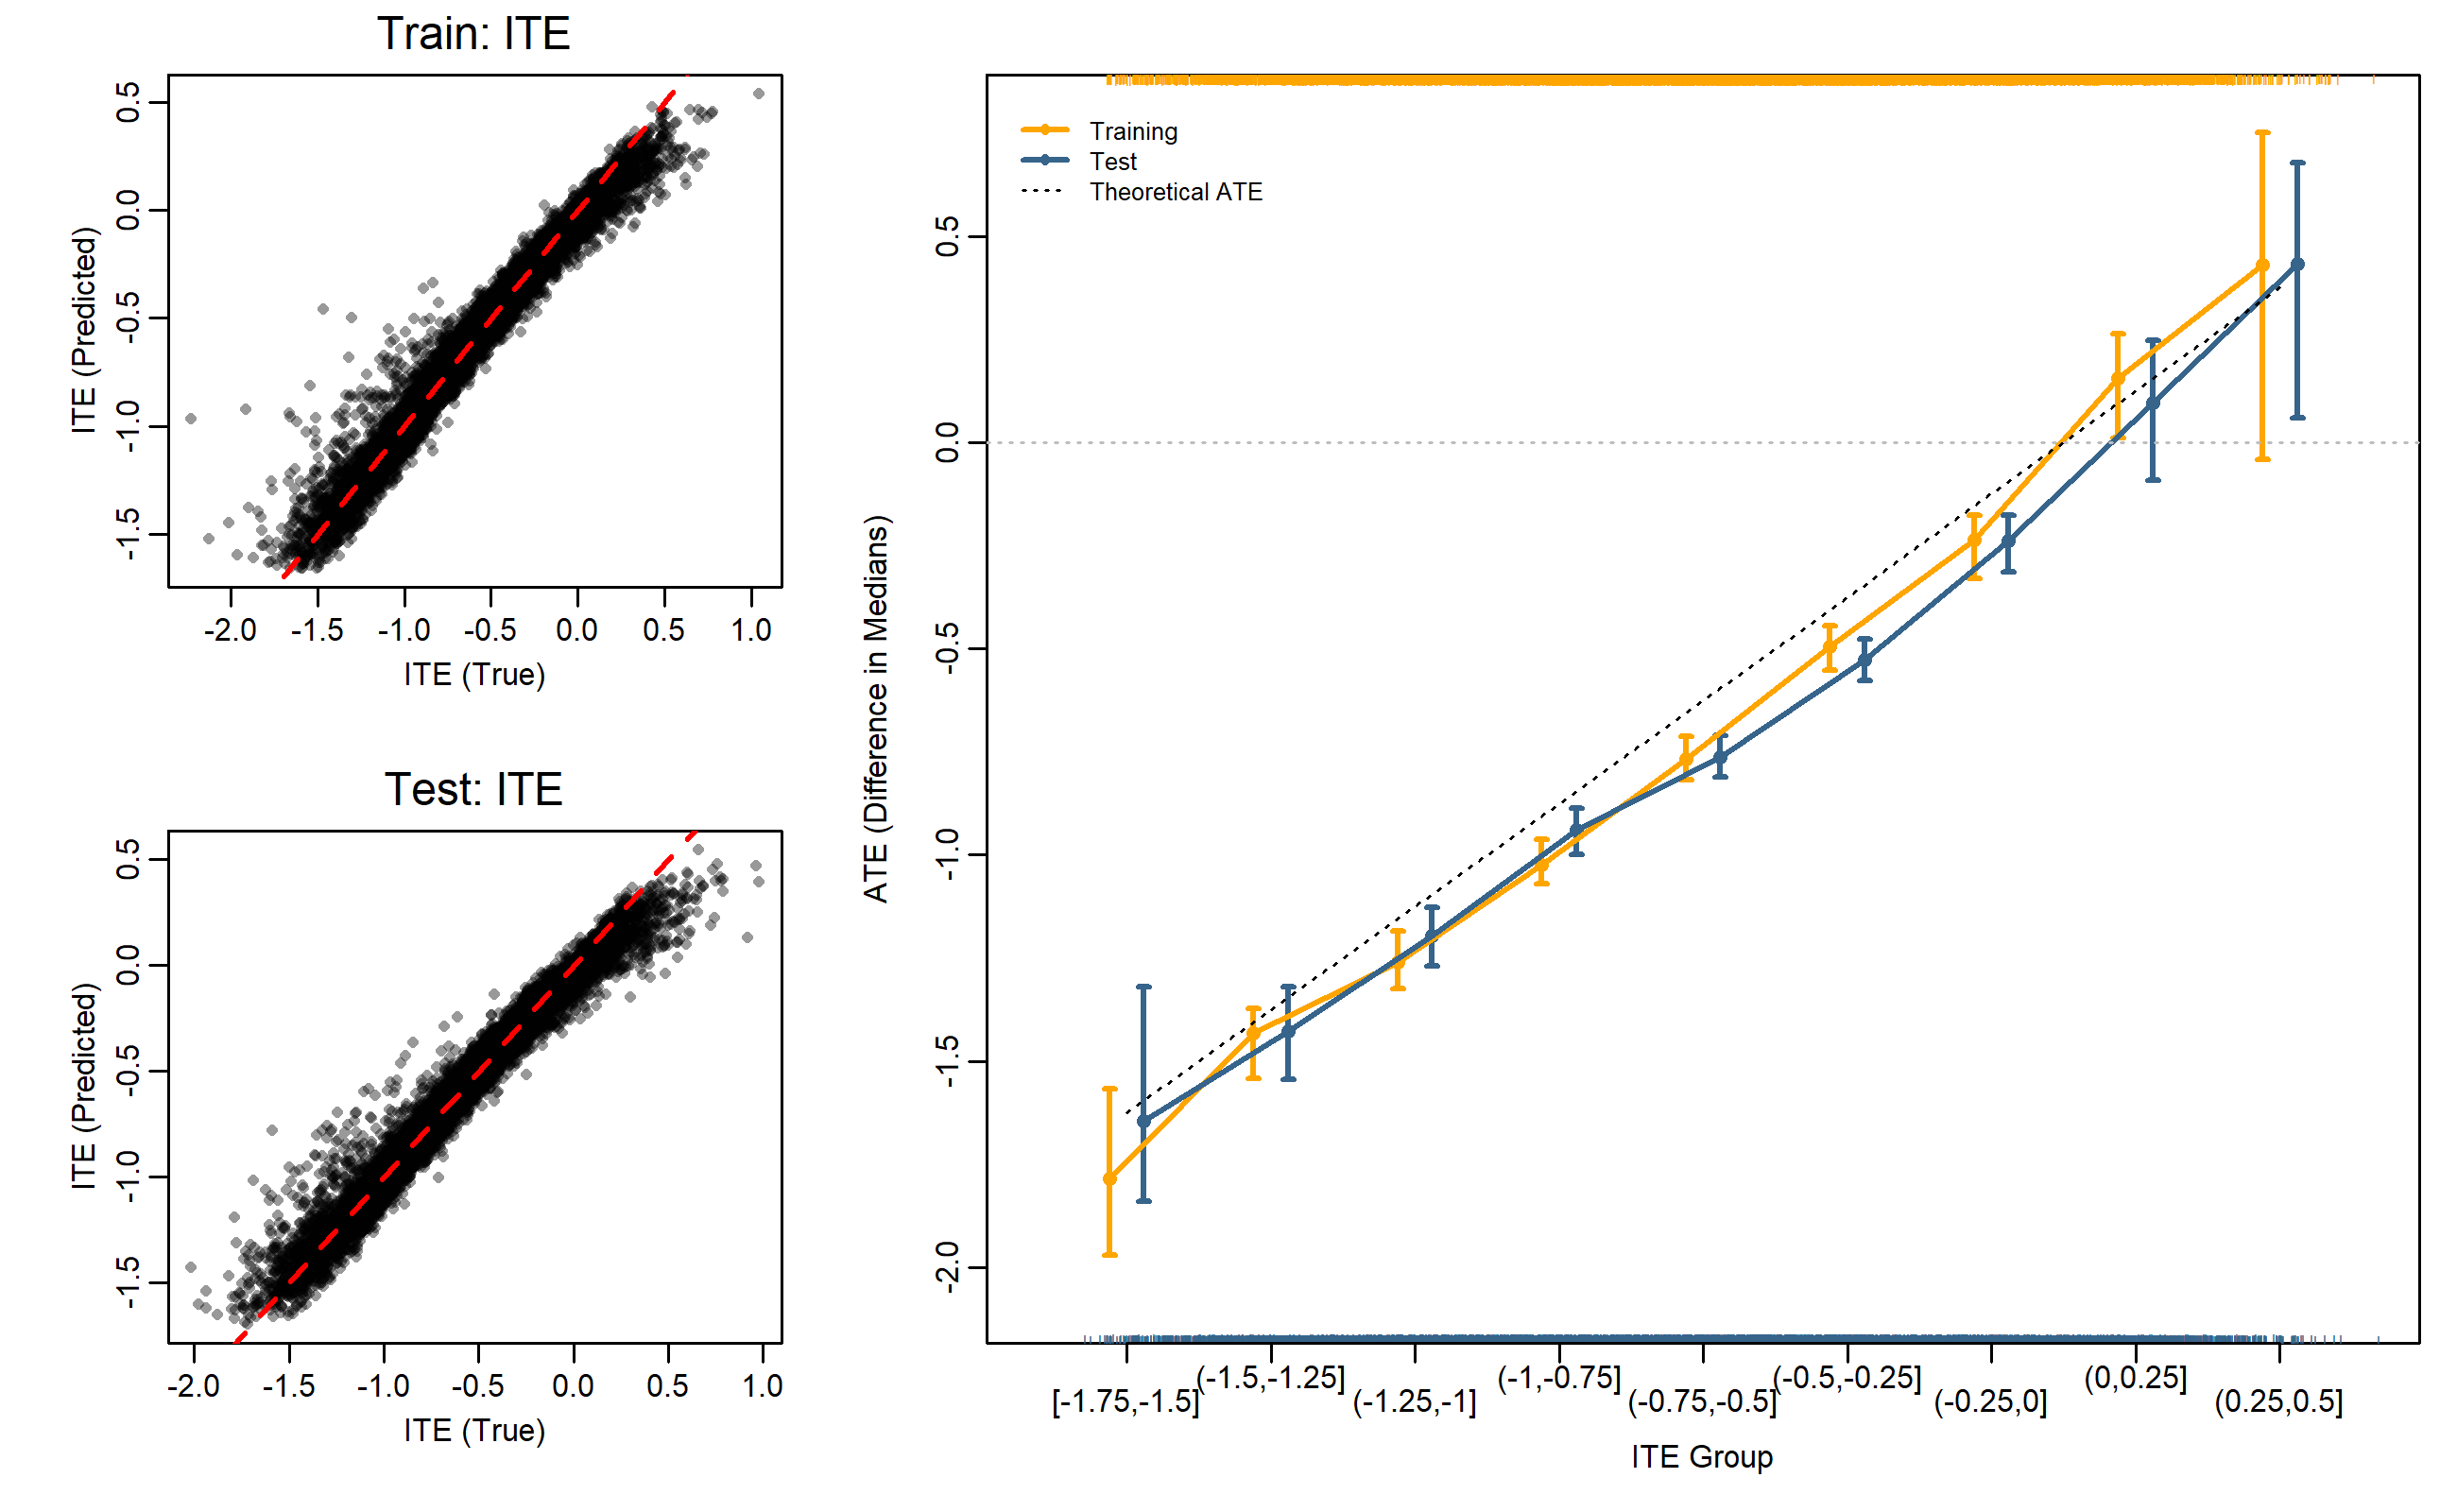
\includegraphics[width=0.9\textwidth]{img/observedITE_ATE_base.png}


\end{frame}




\begin{frame}{TRAM-DAGs: Example for ITE estimation (Results)}



% Comparison of ATE in RCT with $\E(\text{ITE}_{predicted})$


\textbf{ATE TRAM-DAG:} estimated as $\operatorname{mean}(\text{ITE}_{predicted})$:


-0.619 (-0.627 to -0.617)

\vspace{1em}

\textbf{ATE from RCT (randomized:)} estimated as \\ 
observed $\operatorname{median}(Y \mid T = 1)$ - $\operatorname{median}(Y \mid T = 0)$:

-0.637 (-0.662 to -0.610)


\vspace{1em}

\begin{itemize}
    \item confidence intervals obtained by bootstrapping
\end{itemize}






\end{frame}



\begin{frame}{References}
  \small
  \bibliographystyle{apalike}
\bibliography{C:/Users/kraeh/OneDrive/Dokumente/Desktop/UZH_Biostatistik/Masterarbeit/MA_Mike/presentation_report/literature/bibSTA490}
\end{frame}

\end{document}
